\documentclass[11pt]{report}

\usepackage[utf8]{inputenc}
\usepackage{csquotes}

% The rest of your packages...
\setcounter{tocdepth}{3}
\setcounter{secnumdepth}{3}
\usepackage{graphicx}
\usepackage{caption}
\usepackage{subcaption}
\usepackage{appendix}
\usepackage{sectsty}
\usepackage{paperStyle}
\usepackage{titlesec} 
\usepackage{tabularx}
\usepackage{siunitx}
\usepackage{tipa}
\usepackage{textcmds}
\usepackage{multirow}
\usepackage{float}
\usepackage{enumitem}
\usepackage[dvipsnames]{xcolor}
\usepackage{soul}
\usepackage[section]{placeins}
\usepackage{pgffor}
\usepackage{amssymb}
\definecolor{HLColor}{RGB}{230,230,250}
\sethlcolor{HLColor}
\usepackage{tcolorbox}

\usepackage{pgfplots}
\pgfplotsset{compat=1.16}

% Define custom colors
\definecolor{moodNothing}{HTML}{737373}
\definecolor{moodAwful}{HTML}{ff3333}
\definecolor{moodSad}{HTML}{e37b2b}
\definecolor{moodNeutral}{HTML}{ffd31a}
\definecolor{moodGood}{HTML}{55de55}
\definecolor{moodHappy}{HTML}{1a8cff}

% Pie Chart package
\usepackage{pgf-pie}

\usepackage{geometry}
\usepackage{array}
\usepackage{longtable}

\usepackage{listings}
\lstset{
  basicstyle=\ttfamily,
  columns=fullflexible,
  keepspaces=true,
  showstringspaces=false
}

\definecolor{gray100}{rgb}{0.949, 0.949, 0.949}
\definecolor{gray200}{rgb}{0.851, 0.851, 0.851}
\definecolor{gray300}{rgb}{0.749, 0.749, 0.749}
\definecolor{gray400}{rgb}{0.651, 0.651, 0.651}
\definecolor{gray500}{rgb}{0.549, 0.549, 0.549}
\definecolor{gray600}{rgb}{0.451, 0.451, 0.451}
\definecolor{gray700}{rgb}{0.349, 0.349, 0.349}
\definecolor{gray800}{rgb}{0.251, 0.251, 0.251}
\definecolor{gray900}{rgb}{0.149, 0.149, 0.149}

\definecolor{blue100}{rgb}{0.910, 0.957, 1.000}
\definecolor{blue200}{rgb}{0.702, 0.851, 1.000}
\definecolor{blue300}{rgb}{0.502, 0.757, 1.000}
\definecolor{blue400}{rgb}{0.302, 0.651, 1.000}
\definecolor{blue500}{rgb}{0.102, 0.549, 1.000}
\definecolor{blue600}{rgb}{0.000, 0.447, 0.800}
\definecolor{blue700}{rgb}{0.000, 0.333, 0.600}
\definecolor{blue800}{rgb}{0.000, 0.224, 0.400}
\definecolor{blue900}{rgb}{0.000, 0.110, 0.200}

\definecolor{green100}{rgb}{0.918, 0.976, 0.918}
\definecolor{green200}{rgb}{0.773, 0.949, 0.773}
\definecolor{green300}{rgb}{0.631, 0.922, 0.631}
\definecolor{green400}{rgb}{0.482, 0.894, 0.482}
\definecolor{green500}{rgb}{0.333, 0.871, 0.333}
\definecolor{green600}{rgb}{0.271, 0.698, 0.271}
\definecolor{green700}{rgb}{0.204, 0.525, 0.204}
\definecolor{green800}{rgb}{0.141, 0.384, 0.141}
\definecolor{green900}{rgb}{0.071, 0.192, 0.071}

\definecolor{red100}{rgb}{1.000, 0.918, 0.918}
\definecolor{red200}{rgb}{1.000, 0.800, 0.800}
\definecolor{red300}{rgb}{1.000, 0.600, 0.600}
\definecolor{red400}{rgb}{1.000, 0.400, 0.400}
\definecolor{red500}{rgb}{1.000, 0.200, 0.200}
\definecolor{red600}{rgb}{0.800, 0.149, 0.149}
\definecolor{red700}{rgb}{0.600, 0.102, 0.102}
\definecolor{red800}{rgb}{0.400, 0.051, 0.051}
\definecolor{red900}{rgb}{0.200, 0.024, 0.024}

\definecolor{orange100}{rgb}{1.000, 0.953, 0.910}
\definecolor{orange200}{rgb}{1.000, 0.851, 0.749}
\definecolor{orange300}{rgb}{1.000, 0.757, 0.502}
\definecolor{orange400}{rgb}{1.000, 0.675, 0.451}
\definecolor{orange500}{rgb}{0.890, 0.482, 0.169}
\definecolor{orange600}{rgb}{0.800, 0.435, 0.227}
\definecolor{orange700}{rgb}{0.600, 0.333, 0.188}
\definecolor{orange800}{rgb}{0.400, 0.227, 0.122}
\definecolor{orange900}{rgb}{0.200, 0.114, 0.059}

\definecolor{yellow100}{rgb}{1.000, 0.976, 0.910}
\definecolor{yellow200}{rgb}{1.000, 0.937, 0.702}
\definecolor{yellow300}{rgb}{1.000, 0.894, 0.502}
\definecolor{yellow400}{rgb}{1.000, 0.859, 0.302}
\definecolor{yellow500}{rgb}{1.000, 0.827, 0.102}
\definecolor{yellow600}{rgb}{0.800, 0.667, 0.082}
\definecolor{yellow700}{rgb}{0.600, 0.490, 0.063}
\definecolor{yellow800}{rgb}{0.400, 0.322, 0.039}
\definecolor{yellow900}{rgb}{0.200, 0.161, 0.020}


\usepackage{afterpage}
\newcommand\myemptypage{
    \null
    \thispagestyle{empty}
    \addtocounter{page}{-1}
    \newpage
    }

% Set up bibliography
\usepackage[
    backend=biber,
    style=numeric,
    sorting=none
]{biblatex}

% Set the font (output) encoding
\usepackage[T1]{fontenc}

% Greek-specific commands
\usepackage[english]{babel}
\usepackage{alphabeta}

% Use the lmodern font to handle bold/italic Greek correctly
\usepackage{lmodern}

% TOP MARGIN:
\makeatletter
\setlength{\@fptop}{0pt}
\makeatother

% BIBLIOGRAPHY:
\addbibresource{references.bib}

% Global Chapter and Section Font Styling
\titleformat{\chapter}[display]
  {\normalfont\huge\bfseries\color{black}\centering}
  {\chaptertitlename\ \thechapter}{20pt}{\LARGE}

\titleformat{\section}
  {\normalfont\Large\bfseries\color{black}}
  {\thesection}{1em}{}

\definecolor{backcolor}{HTML}{f2f2f2}

\lstdefinelanguage{JavaScript}{
  keywords={typeof, new, true, false, catch, function, return, null, catch, switch, var, if, in, while, do, else, case, break},
  keywordstyle=\color{blue}\bfseries,
  ndkeywords={class, export, boolean, throw, implements, import, this},
  ndkeywordstyle=\color{darkgray}\bfseries,
  identifierstyle=\color{black},
  sensitive=false,
  comment=[l]{//},
  morecomment=[s]{/*}{*/},
  commentstyle=\color{purple}\ttfamily,
  stringstyle=\color{red}\ttfamily,
  morestring=[b]',
  morestring=[b]"
}

\lstset{
   language=JavaScript,
   backgroundcolor=\color{backcolor},
   extendedchars=true,
   basicstyle=\footnotesize\ttfamily,
   showstringspaces=false,
   showspaces=false,
   numbers=left,
   numberstyle=\footnotesize,
   numbersep=9pt,
   tabsize=2,
   breaklines=true,
   showtabs=false,
   captionpos=b
}

\begin{document}

% Roman numerals for the initial pages
\pagenumbering{arabic}
\thispagestyle{empty}

\thispagestyle{empty}

% CUSTOM TITLE
\begin{titlepage}
    \begin{center}
        % Include emblem image at the top
        
\includegraphics[width=0.8\linewidth]{figures/university/logo-english.pdf} \\[5em]

        %  English title
        {\LARGE \textbf{Design and development of a mobile mood tracker application}}\\[10mm]

        % Thesis designation
        {\large \textbf{DIPLOMA THESIS}}\\[5em]

        % Author's name and supervisor
        {\Large \textbf{Alexandros Tsaparas}} \\[1em]
        {\normalsize Registration Number: 1072824} \\[2em] % AM number
        {\large \textbf{\textit{Supervisor}}} \\[0.2em]
        {\large \textit{Christos Sintoris}} \\[2em]

        % Department and University information
        \rule{0.5\textwidth}{0.4pt} \\[1.5em] % A separator line
        {\large Electrical and Computer Engineering Department} \\[0.5em]
        {\large University of Patras}\\[2em]

        % Date at the bottom
        {\large Patras, September 2024}
    \end{center}
\end{titlepage}

\thispagestyle{empty}
\myemptypage
\thispagestyle{empty}

\vspace*{\fill}
\noindent University of Patras, Department of Electrical and Computer Engineering.

\vspace{3mm}

\noindent Alexandros Tsaparas

\vspace{3mm}

\noindent © 2024 – All rights reserved

\vspace{5mm}

\noindent The whole work is an original work, produced by Alexandros Tsaparas, and does not violate the rights of third parties in any way. If the work contains material which has not been produced by him/her, this is clearly visible and is explicitly mentioned in the text of the work as a product of a third party, noting in a similarly clear way his/her identification data, while at the same time confirming that in case of using original graphics representations, images, graphs, etc., has obtained the unrestricted permission of the copyright holder for the inclusion and subsequent publication of this material.

\thispagestyle{empty}
\thispagestyle{empty}

\begin{center}
    \textbf{\LARGE CERTIFICATION}\\[2em]
    
    It is certified that the Diploma Thesis titled \\[1em]
    
    \textbf{\Large Design and development of a mobile mood tracker application} \\[2em]
    
    of the Department of Electrical and Computer Engineering student \\[2em]
    
    \textbf{\large Alexandros Tsaparas, son of Konstantinos} \\[1em]
    
    Registration Number: \textbf{1072824} \\[2em]
    
    was presented publicly at the Department of Electrical and Computer Engineering at \\[2em]
    
    \textbf{14/09/2014} \\[2em]
    
    and was examined by the following examining committee: \\[3em]
    
    \begin{tabbing}
        Christos Sintoris, Laboratory Teaching Staff, ECE Department \hspace{1cm} \= (supervisor) \\
        Christos Feidas, Associate Professor, ECE Department \> (committee member) \\
        Andreas Komninos, Assistant Professor, C.E.I.D \> (committee member)
    \end{tabbing}
    
    \vfill
    
    \begin{minipage}[t]{0.45\textwidth}
        \begin{center}
            \underline{\hspace{5cm}} \\[0.2em]
            The Supervisor \\[3.5em] % Adjusted vertical space for alignment
            Christos Sintoris \\[0.5em]
            Laboratory Teaching Staff
        \end{center}
    \end{minipage}%
    \hfill
    \begin{minipage}[t]{0.45\textwidth}
        \begin{center}
            \underline{\hspace{5cm}} \\[0.2em]
            The Director of the Division of Electronics and Computers \\[1.6em] % Adjusted vertical space for alignment
            Georgios Theodoridis \\[0.5em]
            Associate Professor
        \end{center}
    \end{minipage}    
    
\end{center}

\thispagestyle{empty}
\myemptypage
\thispagestyle{empty}

% CUSTOM TITLE
\begin{titlepage}
    \begin{center}
        % Include emblem image at the top
        \includegraphics[width=0.8\linewidth]{figures/university/logo-greek.pdf} \\[5em]

        % English title
        {\LARGE \textbf{Σχεδίαση και ανάπτυξη φορητής εφαρμογής παρακολούθησης διάθεσης}}\\[10mm]

        % Thesis designation
        {\large \textbf{ΔΙΠΛΩΜΑΤΙΚΗ ΕΡΓΑΣΙΑ}}\\[5em]

        % Author's name and supervisor
        {\Large \textbf{Αλέξανδρος Τσαπάρας}} \\[1em]
        {\normalsize AM: 1072824} \\[2em]
        {\large \textbf{\textit{Επιβλέπων}}} \\[0.2em]
        {\large \textit{Χρήστος Σιντόρης}} \\[2em]

        % Department and University information
        \rule{0.5\textwidth}{0.4pt} \\[1.5em] % A separator line
        {\large Τμήμα Ηλεκτρολόγων Μηχανικών \& Τεχνολογίας Υπολογιστών} \\[0.5em]
        {\large Πανεπιστημιο Πατρών}\\[2em]

        % Date at the bottom
        {\large Πάτρα, Σεπτέμβριος 2024}
    \end{center}
\end{titlepage}

\thispagestyle{empty}
\myemptypage
\thispagestyle{empty}

\vspace*{\fill}
\noindent Πανεπιστήμιο Πατρών, Τμήμα Ηλεκτρολόγων Μηχανικών και Τεχνολογίας Υπολογιστών.

\vspace{3mm}

\noindent Αλέξανδρος Τσαπάρας

\vspace{3mm}

\noindent ©2024 — Με την επιφύλαξη παντός δικαιώματος

\vspace{5mm}

\noindent Το σύνολο της εργασίας αποτελεί πρωτότυπο έργο, παραχθέν από τον Αλέξανδρο Τσαπάρα, και δεν παραβιάζει δικαιώματα τρίτων καθ’ οιονδήποτε τρόπο. Αν η εργασία περιέχει υλικό, το οποίο δεν έχει παραχθεί από τον ίδιο, αυτό είναι ευδιάκριτο και αναφέρεται ρητώς εντός του κειμένου της εργασίας ως προϊόν εργασίας τρίτου, σημειώνοντας με παρομοίως σαφή τρόπο τα στοιχεία ταυτοποίησής του, ενώ παράλληλα βεβαιώνει πως στην περίπτωση χρήσης αυτούσιων γραφικών αναπαραστάσεων, εικόνων, γραφημάτων κ.λπ., έχει λάβει τη χωρίς περιορισμούς άδεια του κατόχου των πνευματικών δικαιωμάτων για την συμπερίληψη και επακόλουθη δημοσίευση του υλικού αυτού.

\thispagestyle{empty}
\thispagestyle{empty}

\begin{center}

    \textbf{\LARGE ΠΙΣΤΟΠΟΙΗΣΗ}\\[2em]
    
    Πιστοποιείται ότι η Διπλωματική Εργασία με τίτλο \\[1em]
    
    \textbf{\Large Σχεδίαση και ανάπτυξη φορητής εφαρμογής παρακολούθησης διάθεσης} \\[2em]
    
    του φοιτητή του Τμήματος Ηλεκτρολόγων Μηχανικών και Τεχνολογίας Υπολογιστών \\[2em]
    
    \textbf{\large Αλέξανδρος Τσαπάρας, του Κωνσταντίνου} \\[1em]
    
    Αριθμός Μητρώου: \textbf{1072824} \\[2em]
    
    Παρουσιάστηκε δημόσια στο Τμήμα Ηλεκτρολόγων Μηχανικών και Τεχνολογίας Υπολογιστών στις \\[2em]
    
    \textbf{14/09/2014} \\[2em]
    
    και εξετάστηκε από την ακόλουθη εξεταστική επιτροπή: \\[3em]
    
    \begin{tabbing}
        Χρήστος Σιντόρης, Εργαστηριακό Διδακτικό Προσωπικό, ΤΗΜ\&ΤΥ \hspace{1cm} \= (επιβλέπων) \\
        Χρήστος Φειδάς, Αναπληρωτής Καθηγητής, ΤΗΜ\&ΤΥ \> (μέλος επιτροπής) \\
        Ανδρέας Κομνηνός, Επίκουρος Καθηγητής, ΤΜΗΥ\&Π \> (μέλος επιτροπής)
    \end{tabbing}
    
    \vfill
    
    \begin{minipage}[t]{0.45\textwidth}
        \begin{center}
            \underline{\hspace{5cm}} \\[0.2em]
            Ο Επιβλέπων \\[3.5em]
            Χρήστος Σιντόρης \\[0.5em]
            Εργαστηριακό Διδακτικό Προσωπικό
        \end{center}
    \end{minipage}%
    \hfill
    \begin{minipage}[t]{0.45\textwidth}
        \begin{center}
            \underline{\hspace{5cm}} \\[0.2em]
            Ο Διευθυντής του Τομέα Ηλεκτρονικής και Υπολογιστών \\[1.6em] 
            Γεώργιος Θεοδωρίδης \\[0.5em]
            Αναπληρωτής Καθηγητής
        \end{center}
    \end{minipage}  
    
\end{center}

\thispagestyle{empty}
\clearpage
\myemptypage
\thispagestyle{empty}

\renewcommand{\abstractname}{\large Abstract}
\begin{abstract}
    In this diploma thesis, a full-stack application, named \textbf{Mood Tracker}, is designed and developed with the purpose of supporting the mental health of university students. The research and development process of the application is based on the principles of Human-Computer Interaction (HCI) and, more specifically, on creating a human-centered design that enhances user experience and usability. The application aims to provide students with a platform for mood tracking and emotional self-reflection, contributing to better understanding and management of their mental health.\vspace{2mm} \\
    The development of the application followed a systematic approach, starting with a detailed literature review to identify the core issues and existing solutions. This was followed by a design phase where personas, user scenarios, and interface mockups were created to define the application's layout and functionalities. The project then proceeded to implementation, covering database structuring and the development of front-end and back-end components, ensuring a seamless and integrated system.\vspace{2mm} \\
    The user experience of the application was evaluated using methods from the human-centered design framework, such as interviews and questionnaires, which provided valuable feedback throughout its development. Upon completion, the resulting prototype is a complete tool that offers university students an accessible means to understand their emotional well-being, fostering self-awareness and promoting a healthier lifestyle in the academic setting.\vspace{5mm} \\
    \textbf{Keywords}: Students' mental health, Mood tracking, Human-Computer Interaction, Human-centered design, Cross-platform application, React Native
\end{abstract}




\clearpage
\myemptypage
\thispagestyle{empty}

\renewcommand{\abstractname}{\large Σύνοψη}
\begin{abstract}
    Στην παρούσα διπλωματική εργασία, σχεδιάζεται και αναπτύσσεται μια ολοκληρωμένη εφαρμογή με το όνομα \textbf{Mood Tracker}, με σκοπό την υποστήριξη της ψυχικής υγείας των φοιτητών. Η διαδικασία ανάπτυξης βασίζεται στις αρχές της Αλληλεπίδρασης Ανθρώπου-Υπολογιστή (HCI) και συγκεκριμένα στη δημιουργία ενός ανθρωποκεντρικού σχεδιασμού που βελτιώνει την εμπειρία του χρήστη και τη χρηστικότητα της εφαρμογής. Η εφαρμογή στοχεύει στην παροχή μιας πλατφόρμας για την καταγραφή διάθεσης και τον συναισθηματικό αυτο-στοχασμό, συμβάλλοντας στην καλύτερη κατανόηση και διαχείριση της ψυχικής υγείας των φοιτητών.\vspace{2mm} \\
    Η ανάπτυξη της εφαρμογής ακολούθησε μια συστηματική προσέγγιση, ξεκινώντας από μια αναλυτική βιβλιογραφική ανασκόπηση για τον εντοπισμό των βασικών προβλημάτων και των υπαρχουσών λύσεων. Στη συνέχεια, ακολούθησε η φάση σχεδιασμού, όπου δημιουργήθηκαν περσόνες, σενάρια χρήσης και πρωτότυπα διεπαφών, καθορίζοντας τη διάταξη και τη λειτουργικότητα της εφαρμογής. H εργασία προχώρησε στην υλοποίηση, καλύπτοντας τον σχεδιασμό της βάσης δεδομένων, καθώς και την ανάπτυξη του front-end και του back-end, διασφαλίζοντας ένα ολοκληρωμένο και ενοποιημένο σύστημα.\vspace{2mm} \\
    Η εμπειρία χρήστη αξιολογήθηκε χρησιμοποιώντας μεθόδους του ανθρωποκεντρικού σχεδιασμού, όπως συνεντεύξεις και ερωτηματολόγια, που παρείχαν πολύτιμες πληροφορίες καθ’ όλη τη διάρκεια της ανάπτυξης. Με την ολοκλήρωση της εργασίας, το τελικό πρωτότυπο αποτελεί ένα πλήρες εργαλείο που προσφέρει στους φοιτητές ένα εύχρηστο μέσο για να κατανοούν την ψυχική τους κατάσταση, προάγοντας την αυτογνωσία και έναν πιο υγιή τρόπο ζωής στο πανεπιστημιακό περιβάλλον.\vspace{5mm} \\
    \textbf{Λέξεις-κλειδιά}: Ψυχική υγεία φοιτητών, Παρακολούθηση διάθεσης, Αλληλεπίδραση Ανθρώπου-Υπολογιστή, Ανθρωποκεντρικός σχεδιασμός, Εφαρμογή cross-platform, React Native
\end{abstract}

\clearpage
\myemptypage
\thispagestyle{empty}

\thispagestyle{empty}
\vspace*{2cm}
\noindent {\large \textbf{Acknowledgments}}

\vspace{5mm}

\noindent As I complete my thesis, I would like to express my heartfelt gratitude to everyone who has contributed to my academic journey.\vspace{3mm} \\
First, I want to thank my supervisor and teacher, Mr. Christos Sintoris, who not only supported me throughout the process but also proposed the idea for this thesis when I first approached him about becoming my supervisor. I would also like to extend my thanks to Mr. Nikolaos Avouris, whose excellent teaching has been a source of inspiration since my first year, providing me with valuable knowledge and guidance that shaped my academic path.\vspace{3mm} \\
Additionally, I would like to thank my classmates and teacher from the ``User Interface Design'' course I attended during my Erasmus semester in Prague, which provided me with valuable insights and knowledge applicable to this project. Special thanks to my friends and fellow students for their constant and effortless support and for encouraging my engagement with the Division of Electronics and Computers throughout my academic journey, as well as for providing valuable feedback during the development of this thesis.\vspace{3mm} \\
In conclusion, I owe deep gratitude to my parents and brother for their continuous support, invaluable ideas, and belief in my abilities.

\clearpage
\myemptypage
\thispagestyle{empty}

\vspace*{2cm}
\noindent {\large \textbf{Ευχαριστίες}}

\vspace{5mm}

\noindent Καθώς ολοκληρώνω τη διπλωματική μου εργασία, θα ήθελα να εκφράσω την ειλικρινή μου ευγνωμοσύνη σε όλους όσοι συνέβαλαν στην ακαδημαϊκή μου πορεία.\vspace{3mm} \\
Πρώτα απ' όλα, θέλω να ευχαριστήσω τον επιβλέποντα και δάσκαλό μου, κ. Χρήστο Σίντορη, ο οποίος όχι μόνο με στήριξε σε όλη τη διάρκεια της διαδικασίας, αλλά και πρότεινε την ιδέα για αυτή τη διπλωματική όταν τον προσέγγισα για να γίνει επιβλέπων μου. Επίσης, θα ήθελα να ευχαριστήσω τον κ. Νικόλαο Αυγουρή, του οποίου η εξαιρετική διδασκαλία αποτέλεσε πηγή έμπνευσης από το πρώτο έτος, παρέχοντάς μου πολύτιμες γνώσεις και καθοδήγηση που διαμόρφωσαν την ακαδημαϊκή μου πορεία.\vspace{3mm} \\
Θα ήθελα επίσης να ευχαριστήσω τους συμφοιτητές και τον δάσκαλό μου από το μάθημα ``User Interface Design'' που παρακολούθησα κατά το Erasmus εξάμηνό μου στην Πράγα, το οποίο μου προσέφερε χρήσιμες γνώσεις και ιδέες που εφαρμόστηκαν σε αυτό το έργο. Ιδιαίτερες ευχαριστίες στους φίλους και συμφοιτητές μου για την αδιάκοπη και αβίαστη υποστήριξη και την ενθάρρυνση να ασχοληθώ ενεργά με τον Τομέα Ηλεκτρονικής και Υπολογιστών σε όλη τη διάρκεια των σπουδών μου, καθώς και για τις πολύτιμες παρατηρήσεις τους κατά την ανάπτυξη αυτής της διπλωματικής εργασίας.\vspace{3mm} \\
Εν κατακλείδι, οφείλω βαθιά ευγνωμοσύνη στους γονείς μου και τον αδερφό μου για τη συνεχή υποστήριξή τους, τις ανεκτίμητες ιδέες τους και την πίστη τους στις ικανότητές μου.

\clearpage
\myemptypage
\thispagestyle{empty}

\tableofcontents

\thispagestyle{empty}
\clearpage
\pagenumbering{arabic} 

\chapter{Introduction}

The primary objective of this thesis is to explore and address the emotional well-being of university students by developing a dedicated mood-tracking application. The aim of the application is to capture the mood of students, offering an insightful tool to understand their psychological state. Through this digital platform, students are able to reflect on their emotional experiences, providing valuable data to better comprehend the factors influencing their overall mood and mental health.\vspace{5mm} \\
In \textbf{Chapter 1}, the motivation behind the project is outlined, discussing the context, goals, and methodologies employed throughout the thesis. This chapter sets the foundation for the research and development process, defining the scope and significance of the proposed solution in the context of supporting student mental health.\vspace{5mm} \\
\textbf{Chapter 2} presents a comprehensive literature review on student mental health and well-being. It includes an analysis of key research studies from universities around the world, examining the primary causes of poor mental health among students. This chapter also introduces the findings from a preparatory survey conducted specifically for this thesis, focusing on academic experiences, social interactions, and general well-being of students. The chapter concludes by comparing these findings to existing mood-tracking applications, identifying gaps and areas for improvement.\vspace{5mm} \\
\textbf{Chapter 3} focuses on the analysis phase of the project. Using the PACT Model, this chapter provides a detailed framework for understanding user needs and expectations. Personas and scenarios are developed based on survey data, highlighting diverse user profiles and interactions. This chapter also includes a comprehensive requirements analysis, defining both functional and non-functional aspects of the application, along with a detailed evaluation of various mood assessment scales to identify the most suitable option for tracking student well-being.\vspace{5mm} \\
\textbf{Chapter 4} is dedicated to the user interface and experience (UI/UX) design of the application. It outlines the design principles and strategies used to create a visually appealing and user-friendly interface. The chapter covers the initial mockup designs, evaluations, and iterations leading to the final design. It also includes a discussion on core design elements such as color palettes, fonts, icons, and animations, as well as inspiration drawn from existing applications to refine the visual and interactive components of the app.\vspace{5mm} \\
\textbf{Chapter 5} digs into the technical implementation of the application. It describes the software architecture, database design, and the integration of front-end and back-end components. This chapter provides a detailed walkthrough of the project setup, coding structure, and the development process, highlighting key technical challenges and solutions encountered during implementation.\vspace{5mm} \\
\textbf{Chapter 6} evaluates the application through user testing and feedback. The chapter outlines the testing methodology, participant selection, and data collection techniques. Results from user tests, interviews, and the User Experience Questionnaire (UEQ) are analyzed to assess the usability and effectiveness of the application. Based on this feedback, recommendations for future improvements are proposed.\vspace{5mm} \\
Finally, \textbf{Chapter 7} concludes the thesis by summarizing the main findings, discussing the overall contribution of the project, and identifying potential future research directions. The chapter reflects on the impact of the mood-tracking application on student mental health and suggests ways to further develop and enhance the system.\vspace{5mm} \\
To summarize, this thesis presents a complete approach to enhance student mood and well-being through the design and implementation of a specialized application, informed by both existing research and user-centered design principles.

\section{Motivation}

The motivation behind my decision to address the issue of student mental health and well-being originates from my personal experience as a student and the observations I have made within my academic environment. While I personally do not suffer from mental health issues, I have witnessed firsthand how this problem affects many of my fellow students. Conversations with friends and peers have revealed the extensive pressure, anxiety, and stress that students often face due to academic expectations, challenging coursework, and a lack of effective support systems. These struggles are not limited only to my close circle or university; they are frequent among students globally, making it clear that mental health is a critical issue in higher education.\vspace{5mm} \\
Seeing people close to me struggle with their mental health and feeling somewhat helpless in supporting them motivated me to explore how technology can offer a practical solution. I believe that addressing this problem is not just about providing immediate assistance, but about creating a sustainable tool that can help students better manage their emotions, track their moods, and become stronger in overcoming emotional challenges.

\section{Context}

The context of the problem revolves around the increasing mental health challenges faced by students in higher education institutions worldwide. University life, often regarded as a crucial period for personal and academic growth, can at the same time become a source of significant stress, anxiety, and emotional tension. The strict academic demands, intense competition, uncertainty about future career paths, and lack of suitable support systems contribute to a challenging environment that negatively impacts students' mental well-being. In addition, the transition from adolescence to adulthood, coupled with social and financial pressures, further escalate the situation, leaving many students struggling to balance their academic responsibilities with personal needs.\vspace{5mm} \\
Despite the commonness of these issues, mental health support within universities is often limited or isn't utilized well. Many students are either unaware of available resources or unwilling to seek help due to shame or fear of being judged. Additionally, the university environment itself—characterized by large class sizes, limited professor-student interaction, and hard communication channels—often fails to provide the personalized attention that students need during periods of emotional difficulty. This context highlights the urgent need for effective tools and interventions that can not only provide support but also empower students to take control of their mental well-being and navigate their university experience in a healthier, more balanced manner. By acknowledging and addressing these underlying factors, we can begin to develop solutions that enhance the overall mental health landscape in academic settings.

\section{Goal (Primary Objective)}

The goal of this thesis is to \textbf{design and develop a complete application tailored specifically to support students in managing their mood and overall well-being throughout their academic journey}. By using findings from preparatory research and a survey conducted among university students, this project aims to identify the key factors affecting students' mental health and translate these findings into actionable features within the application. The primary objective is to create a tool that not only helps students track their mood but also provides them with valuable insights and recommendations, thereby fostering a positive and supportive university environment. Ultimately, this thesis seeks to contribute to the broader discussion on student mental health by offering a practical solution that addresses the challenges faced by students and help for a healthier and more balanced academic experience. Through the development of this application, the thesis aspires to bridge the gap between the existing support systems and the actual needs of students, creating a meaningful impact on their well-being and academic success.

\section{Method}

To complete this thesis project, a structured methodology is followed, covering multiple phases from research to implementation. Based on the motivation, context, and primary objectives outlined in the previous sections, the fundamentals necessary for developing the application were established. This process begins with an in-depth literature review to understand the core challenges and existing solutions for student mental health. Subsequently, the user needs were defined using the PACT model, personas, and user scenarios, which guided the application’s design and functionality.\vspace{2mm} \ After finalizing the design, the implementation phase included database structuring, front-end and back-end development, and deployment to ensure a seamless and robust system. To visualize this process, a sequence diagram showing the various stages of the project is provided below:

\vspace{5mm}

\FloatBarrier
\begin{figure}[ht]
    \centering
    \includegraphics[width=\linewidth]{figures/Sequence-Diagram.pdf}\label{fig:sequence-diagram}
    \caption{Methodology Diagram}
\end{figure}
\FloatBarrier

\vspace{5mm}

\noindent It is important to note that the development process involved multiple iterations between the design and implementation phases. This back-and-forth approach was necessary to address various challenges that arose during implementation, such as technical limitations or usability concerns. These issues were resolved through a recurring process of redesigning and refining, ensuring that the final application aligns closely with the initial objectives and offers a seamless user experience.
\chapter{Literature Review}

\section{Relevant Research}

The following section addresses the relevance of my application and the importance of user research in its development. Specifically, it explores why understanding and improving student mood and well-being is crucial for universities. To this end, various scientific studies and publications were reviewed, along with contributions from health-related organizations. These studies aimed to identify the primary causes behind student struggles, gathering critical insights into the factors affecting their emotional state. Additionally, a thorough analysis of similar applications in the market was conducted to evaluate existing features, limitations, and opportunities for innovation. This research sought to pinpoint gaps in current solutions and identify novel ideas that could enhance the user experience. Moreover, a targeted survey was carried out to gather specific user needs and preferences, ensuring that the app's design directly addresses the challenges faced by students.\vspace{5mm} \\
In the course of my user research, I found numerous sources that prove that student well-being is directly related to their productivity. Numerous universities globally invest resources in understanding the intricate connection between students' mental health, stress levels, and academic performance. Additionally, beyond academia, researchers from various fields explore well-being across demographics, employing diverse methodologies such as surveys and longitudinal studies.

\FloatBarrier
\begin{table}[ht]
\centering
\begin{tabular}{|p{4cm}|p{10cm}|}
\hline
\textbf{Research} & \textbf{Summary} \\ \hline
University of Applied Sciences, Northern Netherlands. & This study focused on understanding the key factors affecting student well-being during the COVID-19 pandemic. It identified mental health issues such as anxiety, academic pressure, and inadequate support as major challenges for students. \\ \hline
Renmin University of China, Haidian, Beijing, China. & The research tracked students over four years to evaluate their mental health using the DASS-21 scale. It revealed fluctuations in anxiety, depression, and stress levels, with anxiety peaking in early academic years and improving in later years. \\ \hline
Indonesian Private Universities. & This study examined the relationship between students' emotional states (positive and negative moods) and their academic performance. It found that negative mood significantly hinders learning, while positive mood had no strong effect. The learning process strongly impacted academic outcomes. \\ \hline
The Student Well-being Model. & The study presents a comprehensive model of student well-being, integrating emotional, academic, and social dimensions. It emphasizes the need for a holistic approach to supporting student well-being. \\ \hline
Hascher's Research. & This research highlights the lack of specific tools to measure student well-being and introduces innovative methods such as multi-faceted questionnaires and emotion diaries to assess well-being comprehensively. \\ \hline
\end{tabular}
\caption{Summary of Key Researches on Student Well-being}
\label{tab:research_summary}
\end{table}
\vspace{5mm}
\FloatBarrier

\subsection{University of Applied Sciences, Northern Netherlands}

Researchers aimed to understand the key factors affecting student well-being, particularly during the challenging period of the COVID-19 pandemic \cite{research-1}. Their goal was to identify the main causes behind the mental and emotional struggles students face, including issues such as anxiety, academic pressure, inadequate support from the university, physical and mental health problems, and social difficulties. By focusing on these factors, the study sought to provide insights into how universities can better support student well-being and address the multifaceted challenges that impact their academic and personal lives.

\vspace{5mm}

\noindent \textbf{Method} \\
A total of 113 students signed up for interviews, selected through purposive sampling based on criteria like full-time status, well-being problems, and diverse representation. They were surely informed from researchers (intranet messages) and Heads of School. Participants were from various academies, study years, and genders. Interviews, lasting 28 to 52 minutes, explored student well-being and related factors. Consent was obtained, and interviews were video recorded. The semi-structured guide covered topics such as defining well-being and factors influencing it. Data collection continued until saturation, with 27 students interviewed.

\vspace{5mm}

\noindent \textbf{Analysis} \\
Thematic analysis was used to interpret data, involving verbatim transcription, member checks, and independent coding by three researchers. Coding was initially done line by line using an open coding approach, with the possibility of applying multiple codes to a passage. Codes were then organized into categories based on data and literature concepts, forming themes. Categories, themes, and data allocation were verified in the final phase by two other researchers to ensure clarity and consistency. Discussions resolved any discrepancies until an agreement was reached.

\vspace{5mm}

\noindent \textbf{Results} \\
Participated five male students, twenty-one female students, and one non-binary student, all aged between 17–24 years, participated. There was revealed a diverse range of self-reported well-being issues among the participating students. These included challenges such as inadequate support from the school, anxiety disorders, family-related issues, physical health problems, symptoms of depression, gender dysphoria, fatigue, and performance anxiety. Additionally, factors like stress, planning difficulties, study pressure, loneliness, perfectionism, and getting used to studying were frequently mentioned by the students. Some participants highlighted the impact of life phase-related problems, ADHD, and drug use on their well-being. The findings underscore the complexity and multifaceted nature of the well-being issues faced by students, emphasizing the need for a holistic approach in addressing these concerns, both within and beyond the academic environment.

\vspace{5mm}

\noindent \textbf{Students' opinions} \\
They expressed diverse views on student well-being. Initially, some found it challenging to define, but as interviews progressed, themes emerged. Well-being was associated with managing stress, achieving balance in academic and personal life, and acknowledging the effort-achievement ratio. Stress and resilience were central themes, with students emphasizing the need to cope with challenges. Well-being was seen as a combination of mental, physical, and social aspects, with support from the university playing a crucial role. Students acknowledged the fluctuating nature of well-being and its significant impact on academic performance.

\vspace{5mm}

\noindent \textbf{Main Factors} \\
The main factors influencing student well-being include self-regulation, perfectionism, motivation levels, ability to plan, and study achievements at the individual level. \textbf{Fellow students} contribute to well-being through practical support, idea exchange, enjoyment, and fostering a community atmosphere. \textbf{Tutors} play a crucial role with good relationships, trustworthiness, accessibility, and time availability. \textbf{Attitudes} and \textbf{behaviors} such as empathy, guidance, and personal attention also influence well-being. \textbf{Teachers} impact well-being through good relationships, accessibility, informal contact, community atmosphere, and attitudes like reassurance, understanding, and recognition. Study-related factors include clear communication, flexibility, workload, and the scale of education. The \textbf{university's} support facilities and community atmosphere are significant. \textbf{Peers} outside the university contribute to well-being through enjoyment, idea exchange, understanding, and recognition. \textbf{Family} support, idea exchange, and enjoyment are also key factors.

\subsection{Renmin University of China, Haidian, Beijing, China}

The university conducted research on students' well-being, recognizing the importance of mental health in maintaining overall health \cite{research-2}. The study addresses the global rise in depression and anxiety cases, particularly among college students. College is identified as a critical period for shaping values, and students' emotional well-being is linked to various factors.

\vspace{5mm}

\noindent \textbf{Method} \\
This study employed data from the ``Beijing College Student Panel Survey'' within the ``China Education Panel Survey'', focusing on the 2008 cohort of students tracked for four years from 2009 to 2012. Sampling involved 15 universities, and the effective sample size was 1401 students. The investigation utilized the Depression Anxiety Stress Scales-21 (DASS-21) to assess psychological well-being, a self-report measure known for its reliability. The DASS-21 includes three scales for depression, anxiety, and stress, each comprising seven items. Scores are calculated by summing corresponding item scores. Notably, the DASS-21's short version requires scores to be multiplied by two for comparison with conventional severity ratings. The study reported good validity for the DASS measurement, supported by scale reliability coefficients of 0.813 for depression, 0.766 for anxiety, and 0.812 for stress. Overall, the methodology involved a comprehensive survey approach, online and on-site rounds, and rigorous measures for assessing students' mental health across their college years.

\vspace{5mm}

\noindent \textbf{Results} \\
The results from the study, provide insights into the mental well-being of Chinese college students across four academic years. The average scores for depression and stress, ranging between 7.22 and 7.79 for depression and 9.53 and 11.68 for stress, consistently fell within the normal range based on cutoff values. However, anxiety scores in the first three years slightly surpassed the normal threshold of 7, with mean scores of 7.40, 7.24, and 7.10, indicating above-average anxiety levels. The previously mentioned statistic numbers, as they increase they reflect more and more the severity of depressive and stress-related symptoms. Interestingly, anxiety levels seemed to decrease in the senior year, with a mean score of 6.63. Despite above-normal anxiety levels in the initial years, students maintained mental health with depression and stress scores in the normal range. The study suggests a fluctuation in mental states, with students experiencing higher stress and depression in the sophomore year, while improvements were observed in the last two years. These findings shed light on the dynamic nature of college students' mental well-being over their academic journey, emphasizing the need for targeted interventions and support to enhance mental health throughout their college experience.

\vspace{5mm}

\noindent \textbf{Discussion and Conclusion} \\
In conclusion, the study sheds light on the mental well-being of Chinese college students over four academic years. Freshmen and sophomores exhibited more mental health challenges, possibly stemming from adjustment issues and increased study pressures. Financial concerns were identified as a significant contributor to anxiety, with Chinese students having relatively lower financial burdens compared to their UK counterparts. Notably, the study revealed differences in psychological well-being trends between China and the US, emphasizing the need for tailored interventions. The longitudinal approach strengthened the credibility of the findings, highlighting grade-related disparities. Key conclusions include the average mental health of Chinese college students, their vulnerability to anxiety in the initial years, and the improvement in psychological well-being over time. The study recommends targeted psychological guidance for different academic years, emphasizing the importance of addressing anxiety in freshmen and enhancing well-being support for sophomores. Future research may explore students' mental changes after entering the workforce for further insights into the development of psychological well-being counseling programs in college.

\subsection{Research on Indonesian Private Universities}

The study explores the relationship between students' emotional states — positive and negative moods — and their academic performance in the context of higher education \cite{research-3}. The research aims to uncover how emotional factors such as mood impact the learning process and, ultimately, students' performance in assessments.

\vspace{5mm}

\noindent \textbf{Method} \\
The study investigated how university students' emotional states—both positive and negative moods—impact their learning process and subsequent academic performance. A total of 116 questionnaires were distributed to students at Indonesian private universities, with 106 valid responses collected (86\% response rate). To minimize external influences on their emotional states, the survey was conducted a week before the students' midterm exams.\\
The study used Likert scale-based questionnaires to measure:

\begin{itemize}
    \item \textbf{Positive and Negative Moods}: Each mood was assessed using six items, rated on a scale from 1 (strongly disagree) to 5 (strongly agree).
    \item \textbf{Learning Process}: Self-reported metrics included attendance, assignment submission, pre-class preparation, post-class review, group discussions, and consultations with teachers, also measured on a 5-point scale.
    \item \textbf{Academic Performance}: This was proxied using midterm examination scores.
\end{itemize}

\noindent The study aimed to assess whether students' moods (positive or negative) influenced their engagement with learning activities, which in turn could predict their exam performance. The study used \textbf{structural equation modeling (SEM)} to explore these relationships and analyzed the data for reliability and validity using techniques like convergent validity, composite reliability, and \textbf{average variance extracted (AVE)}.

\vspace{5mm}

\noindent \textbf{Results} \\
The results showed some interesting patterns:

\begin{itemize}
    \item \textbf{Positive Mood}: Contrary to the hypothesis, positive mood did not significantly influence the learning process. Students in a good mood were not necessarily better at engaging with their academic tasks.
    \item \textbf{Negative Mood}: The data revealed a significant negative relationship between a bad mood and the learning process. Students experiencing negative emotions like sadness or stress were less engaged in learning activities, which directly impacted their academic preparation.
    \item \textbf{Learning Process and Academic Performance}: There was a strong positive relationship between the quality of the learning process and academic performance. Students who participated actively in class discussions, submitted assignments, and reviewed study materials performed better in their midterm exams.
\end{itemize} 

\vspace{5mm}

\noindent \textbf{Conclusion} \\
The study's findings highlight the complexity of the relationship between emotions and academic performance:

\begin{itemize}
    \item \textbf{Positive mood}, while often considered beneficial, did not necessarily promote better learning outcomes in this study.
    \item \textbf{Negative mood} had a clear negative impact on learning, suggesting that addressing emotional difficulties could improve academic engagement.
    \item \textbf{Learning behaviors} remained a critical factor in determining academic success, emphasizing the importance of promoting strong study habits among students regardless of their emotional state.
\end{itemize} 

\noindent The study also provided several practical recommendations:

\begin{itemize}
    \item \textbf{For educators}: Teachers and lecturers should focus on creating a conducive and supportive learning environment that fosters positive student emotions. A pleasant atmosphere and effective teaching strategies can help students stay motivated and engaged.
    \item \textbf{For students}: Students are encouraged to develop resilience and discipline in managing their emotions. Even when experiencing a bad mood, students should try to maintain productive study habits to avoid the negative impact on their academic performance.
\end{itemize} 

\noindent The research ultimately supports the importance of addressing both emotional well-being and learning processes to improve academic outcomes. Although positive mood did not show the expected benefits, ensuring students have strong study habits and the emotional support they need remains essential for their success.

\subsection{Concluding Insights on Student Well-Being in Higher Education}

The exploration of various university research studies on student well-being reveals a complex landscape of mental health challenges faced by students in higher education. Douwes et al. \cite{research-1} and Liu et al. \cite{research-2} emphasize the importance of understanding student well-being from their own perspective. Their research highlights how academic expectations, workload pressures, and examination stressors cause significant psychological fluctuations, demonstrating the need for effective strategies to help students monitor and reflect on their emotional states.\vspace{5mm} \\
Similarly, Febrilia et al. \cite{research-3} explore the link between emotional well-being and academic outcomes, showing that negative moods can severely impact focus and engagement. These insights indicate the critical role of understanding emotional barriers to learning and the potential benefits of tools that track such changes.\vspace{5mm} \\
Furthermore, the “student well-being model” proposed by Soutter et al. \cite{research-4} and the findings by Hascher \cite{research-5} validate the need for comprehensive well-being indicators and assessment tools. Hascher’s study particularly suggests the value of multi-faceted questionnaires and emotion diaries, which can help students better assess their emotional states and academic pressures.\vspace{5mm} \\
Overall, these studies emphasize the necessity of a powerful framework for understanding and addressing the mental health issues of students, which could lead to better support strategies and improved academic outcomes. With this understanding in place, the next step involves applying these insights to design a practical solution for monitoring and supporting student well-being.

\subsection{From the Problem to the Solution}

Building upon these research findings, it is clear that the need for an effective solution to support student well-being is mandatory. In response to this, I decided to design and implement an application, called \textbf{Mood tracker}, aimed at solving the problem of poor mood and well-being among university students. This application will track and project students' emotional states in real time, providing them with tools for self-reflection and helping them be aware of their mood patterns. By enabling students to monitor their course of emotions, the app will empower them to take significant steps toward improving their mental health.

\section{Preparatory Survey}

Despite the relevant research that reviewed existing studies on student well-being and explored the key factors contributing to mental health challenges in universities, it became clear that a custom survey was needed to gain deeper insights into our specific context. While previous researches provided valuable information about the general state of well-being in higher education, it lacked a targeted focus on the influence of teachers, courses, and the university environment on student mental health. To address this gap, I designed a survey to gather direct feedback from students about these aspects.

\subsection{Procedure}

The participants involved in the study were students from various universities and age groups, selected through a convenience sampling method, which included friends and relatives, to represent a versatile view of the university environment. A questionnaire survey was designed, comprising a total of 17 questions (12 mandatory and 5 optional), focusing on different aspects of the student experience. The topics covered by the survey included:

\begin{itemize}
    \item \textbf{Personal Information:} Basic details like the participant’s field of study and current academic year.
    \item \textbf{Academic Experience:} Ratings of overall satisfaction with the academic experience, workload, and feedback on assignments, assessments, or exams.
    \item \textbf{Extracurricular Activities:} Participation in extracurricular activities and their impact on the overall university experience.
    \item \textbf{Mental Health Resources:} Awareness and utilization of mental health resources available on campus.
    \item \textbf{Communication Dynamics:} The preferred communication channels with professors, frequency of communication, and obstacles encountered when interacting with faculty members.
    \item \textbf{Improvements and Suggestions:} Ideas for enhancing the academic experience, the feedback process, and any additional features or tools that could be implemented to engage students better.
\end{itemize}

\noindent The questionnaire was distributed to participants through social media platforms, such as Instagram, Messenger, and WhatsApp, with a completion deadline of one week. Participants were informed that the survey was anonymous and that their responses would be used solely for research purposes.

\subsection{Results}
Eleven students responded to the questionnaire, and in the following section, we discuss the key findings for each topic covered in the survey.

\vspace{5mm}

\noindent \textbf{Field and Year of Study of the participants} \\
The majority of participants are enrolled in Electrical and Computer Engineering indicating a strong representation in this field. Business Engineering and Architecture each constitute of the respondents, showcasing a diverse academic landscape within the surveyed population. Also the fifth academic year is predominant, followed by the third and the sixth years. This distribution may suggest a concentration of survey participants in the latter stages of their academic journey.

\vspace{5mm}

\noindent \textbf{Academic Experience} \\
A considerable number of respondents ($\approx$ 5/10 people) reported a satisfaction rating of 7/10 for their overall academic experience, while approximately 3/10 people reported a rating of 5/10, which means that they are neither satisfied nor dissatisfied. The bulk of participants also considered the workload to be quite substantial, with roughly 5/10 individuals rating it as an 8/10, highlighting the considerable challenges students face in managing their academic responsibilities. We can also observe that most people, around 8/10, take part in after-school activities, and they believe these activities are beneficial. This indicates that being involved in these extra activities not only helps with their studies but also supports overall personal growth. Additionally, 5 out of 10 people expressed dissatisfaction with the feedback mechanisms for communication with professors, indicating potential areas for improvement in this aspect.\vspace{5mm} \\
Notably, a significant proportion of respondents ($\approx$ 9/10 people) identified limited office hours and cited a lack of response to emails as obstacles when trying to communicate with professors. Furthermore, the survey brought to light that  of students are not aware of or have not utilized mental health resources on campus, emphasizing the importance of enhancing awareness and accessibility to support services for the well-being of students. Furthermore, near half of the participants ($\approx$ 4/10 people) reported low numbers about the feedback they receive from their professors about assignments, assessments, and exams, underscoring the need for more comprehensive feedback mechanisms to support students' academic growth and development. According to the contestands, academic stress stems from diverse sources, including the pressure of exams, particularly retakes, heavy workloads, simultaneous deadlines for exams and projects, uncertainties about the future and chosen fields, and concerns about study methods.

\vspace{5mm}

\noindent \textbf{Communication Dynamics} \\
The survey data highlights a significant reliance on feedback from surveys among students, with approximately 5/10 indicating a preference for this communication method over email, online platforms, and in-person office hours. However, despite this preference, half of the students express dissatisfaction with the current feedback mechanisms for communication with professors. This apparent contradiction suggests that while surveys may be a commonly used tool, there might be room for improvement in the effectiveness and responsiveness of the feedback channels.\\ \\
Furthermore, the data indicates a concerning trend regarding student-professor interaction. A majority of students ($\approx$ 8/10) do not feel the need to communicate with their professors, attributing it to a lack of connection. This lack of connection may be influenced by factors such as limited office hours (voted by 10 out of 11 students) and a perceived lack of response to emails ($\approx$ 8/10). The overwhelming use of email as the primary mode of communication ($\approx$ 9/10) suggests that despite its prevalence, students may be facing challenges in establishing meaningful connections and receiving timely support from their professors. Addressing these issues could potentially enhance student engagement and overall satisfaction with the communication channels.

\vspace{5mm}

\noindent \textbf{Improvements and Suggestions} \\
The students provided insightful suggestions for improving their academic experience. A common theme is the need for better support and the normalization of struggles. Students expressed a desire for more advertised support systems and a less stressful environment, suggesting that school hours should be treated as work hours, allowing for a balance between academic and personal time. Another prevalent suggestion is for more transparency in scheduling and a shift towards hands-on learning, with exams conducted through projects rather than traditional methods. Students also emphasized the importance of better organization, materials, and professor approachability, with a call for a rethinking of the teaching process, including more hands-on experiences and the incorporation of young educators. In terms of feedback, students advocated for more active participation and consideration of survey results, hoping for a systematic and regular feedback process that leads to tangible improvements. Lastly, they suggested the implementation of features such as more frequent feedback, increased use of existing tools like Zoom and Skype, and availability of online office hours through apps for better student engagement. These suggestions collectively highlight the students' desire for a more supportive, practical, and engaging academic environment.\vspace{5mm} \\
One of the participants, a student from Germany, said that:

\vspace{5mm}

\noindent Translated Text from German to English \\
\textit{``At my university there are at least a few offers that support students with mental health problems and offer help with certain problems. Some of these offers are provided by the university itself and some are organized as university groups. Although this primarily has to do with the students independently of the teachers, it certainly offers a good opportunity to strengthen the well-being of students. Above all, the advertising and awareness of the offers would have to be increased in order to make the topic of mental well-being much less taboo.''}

\vspace{5mm}

\noindent \textbf{Additional Thoughts} \\
The students express a variety of perspectives on their satisfaction with university settings. One student appreciates the mental health support services available at their university, emphasizing the importance of raising awareness to destigmatize discussions around well-being. Another underscores the need to foster a sense of community among students to enhance their overall happiness in the university environment. On the other hand, some students highlight practical concerns, such as the desire for more office hours for both teachers and secretaries, improved infrastructure, and larger amphitheatres. Additionally, there is a shared sentiment that the university authorities may not fully grasp the challenges faced by the student body, whether in terms of their numbers or the need for responsive actions. These diverse perspectives shed light on various dimensions of student satisfaction, from mental health support to community building and infrastructure improvements, suggesting that a holistic approach is necessary for an optimal university experience.

\subsection{Conclusion}
The results of the survey provide a clearer understanding of the significance of well-being in university environments. The feedback from students reveals a common concern that universities are not addressing mental health issues sufficiently, which are often caused or exacerbated by academic pressures. Many students highlighted that professors and course structures contribute to increased stress, anxiety, and even depression, yet there appears to be a lack of effective measures to counter these issues. For example, students frequently cited heavy workloads, deficient feedback, and limited availability of professors as factors impacting their mental health. Additionally, limited awareness and access to mental health resources on campus were noted as significant barriers to receiving support. This insight emphasizes the need for an effective tool that can assist students in managing their mental health, as current university support systems are perceived as insufficient.\vspace{5mm} \\
Therefore, it is crucial to design and implement a tool that can help students navigate their daily struggles by tracking and understanding their moods. Such a tool would not only provide support but also serve as a guide to enhance their overall university experience. So I decided to design and implement an application aimed at solving the problem of poor mood and well-being among university students. This application can track and project students' emotional states in real time, providing them with tools for self-reflection and helping them be aware of their mood patterns. By enabling students to monitor their course of emotions, the app can empower them to take significant steps toward improving their mental health.

\section{Comparative Analysis of Existing Mood-Tracking Apps}

Given our decision to create an application, it is essential to conduct research on existing state-of-the-art mood-tracking applications that are both popular and well-designed. This research help us gain a deeper understanding of the features that are already available, which we can incorporate into our own application while adding new and innovative elements. To achieve this, I review some of the leading mood-tracking and mental health applications of 2023. These applications showcase a wide range of functionalities and serve as valuable references for identifying current trends in mood tracking.\vspace{5mm} \\
In addition to my own analysis, I include reviews from specialized mental health professionals and app testers. These expert opinions can provide an overall view of each application’s strengths and areas for improvement, offering diverse perspectives on user experience, functionality, and overall design. A brief overview of these applications is summarized in the table below, followed by a detailed comparative analysis based on user feedback, expert reviews, and my personal evaluation.

\FloatBarrier
\begin{table}[ht]
\centering
\begin{tabular}{|p{2cm}|p{6cm}|p{6cm}|}
\hline
\textbf{App} & \textbf{Purpose} & \textbf{Main Features} \\ \hline
Moodfit & A mental health app aimed at improving mood and managing symptoms of stress, anxiety, and depression. Supports users in building healthy habits through CBT-based tools. & Mood journal, daily goals, breathing exercises, mindfulness meditation, medication tracking, lifestyle tracking, therapy companion, summary reports. \\ \hline
Worry Watch & A CBT-based app designed to help users manage anxiety by journaling worries and using mindfulness-based coping tools. & Guided journaling, coping tools, thought diary, affirmations, guided meditation, reminders, privacy controls. \\ \hline
MoodTools & A self-guided mHealth app aimed at managing depression symptoms, with tools for self-monitoring and cognitive restructuring. & PHQ-9 depression test, thought diary, activities tool, videos, safety plan, psychoeducation. \\ \hline
eMoods & A specialized bipolar mood tracker that helps users log mood states, track symptoms, and manage bipolar disorder. & Mood tracking, behavioral logging, symptom rating, graphical reports, custom notes, report generation, daily reminders. \\ \hline
MoodKit & A CBT-based app designed to help users manage depression, anxiety, and stress through structured activities and journaling. & Activities, thought checker, mood tracking, journal, thrive tips, goal tracking. \\ \hline
Daylio & A mood-tracking and journaling app that uses icons and lists to help users track moods and habits quickly without extensive writing. & Mood tracking, activity and habit tracking, statistics hub, customization options, reminders, data exporting, achievements and streaks. \\ \hline
\end{tabular}
\caption{Overview of Mental Health and Mood-Tracking Apps}
\label{tab:overview_mood_apps}
\end{table}
\FloatBarrier

\subsection{Moodfit}

\textbf{\href{https://www.getmoodfit.com/}{Moodfit}\footnote{Link: \url{https://www.getmoodfit.com/}}} is a mental health and wellness app designed to help users improve their mood and manage symptoms of mental health issues like stress, anxiety, and depression \cite{moodfit-review}. Recognized as the ``Best Overall Mental Health App of 2020'', Moodfit offers a variety of tools aimed at promoting emotional well-being. These tools include cognitive behavioral therapy (CBT)-based journaling, daily goal tracking, mindfulness meditation, breathing exercises, and medication tracking. The app supports users in building healthy habits and provides insights into lifestyle factors like sleep, exercise, and nutrition, all of which contribute to mental health.\vspace{5mm} \\
Users can track their emotions with the mood journal feature, allowing them to monitor their emotional patterns and share insights with therapists for a better understanding of their mental state. The app also offers personalized reports, progress charts, and reminders to help users stay on track with their goals. While the app is free to download, premium features are available through in-app purchases.\vspace{5mm} \\
Overall, Moodfit is praised for its well-designed interface, personalized mental health tools, and supportive features like notifications and inspirational articles. However, it does have a few drawbacks, such as the lack of some advanced features and occasional slow performance. Despite these limitations, Moodfit remains a valuable and cost-effective tool for anyone seeking to improve their mental health through daily self-care practices.\vspace{5mm} \\
Here is a summary of the features offered by the application:\vspace{5mm}

\FloatBarrier
\begin{table}[ht]
\centering
\begin{tabular}{|p{4cm}|p{10cm}|}
\hline
\textbf{Feature} & \textbf{Description} \\ \hline
Mood Journal & Allows users to track their mood daily and process their thoughts using a journal based on cognitive behavioral therapy (CBT) techniques. \\ \hline
Daily Goals and Self-care & Encourages users to set daily mental health goals and practice self-care activities that promote well-being. \\ \hline
Breathing Exercises & Provides guided breathing exercises to reduce stress and anxiety, improving emotional regulation. \\ \hline
Gratitude Journal & Encourages users to log things they are grateful for, helping to foster a more positive mindset. \\ \hline
Mindfulness Meditation & Offers mindfulness-based meditation exercises that help users stay present and calm. \\ \hline
Medication Tracking & Helps users track their medications and the effects or side effects related to mood or mental health. \\ \hline
Sleep and Lifestyle Tracking & Allows users to monitor aspects of their lifestyle like sleep, nutrition, and exercise, and how these factors affect their mood. \\ \hline
Therapy Companion & Enables users to share mood charts and progress reports with therapists or coaches to assist in therapy sessions. \\ \hline
Summary Reports & Provides users with downloadable weekly or monthly reports to track their progress and identify patterns in their behavior and mood. \\ \hline
\end{tabular}
\caption{Summary of Features in the Moodfit App}
\label{tab:moodfit_features}
\end{table}
\FloatBarrier

\subsection{WorryWatch}

The \textbf{\href{https://worrywatch.com/}{Worry Watch}\footnote{Link: \url{https://worrywatch.com/}}} app is designed as a cognitive behavioral therapy (CBT)-based tool to help users manage anxiety by journaling their worries, identifying cognitive distortions, and using mindfulness-based coping skills \cite{worrywatch-review}. The review, written by a licensed psychologist, provides insight into the app's effectiveness over a month of testing. The app's features include guided journaling prompts, anxiety tracking, coping mechanisms such as breathing exercises, grounding techniques, and guided meditations.\vspace{5mm} \\
The reviewer appreciated the app's simple and customizable features, such as the breathing exercises and mindfulness tools, which helped in managing daily anxiety. However, concerns were raised regarding the lack of involvement of mental health professionals in the app's development. The app offers both a free version and a paid version, with the free version having limited features, such as restricting the number of journal entries per day.\vspace{5mm} \\
Despite the lack of professional development input, the reviewer found Worry Watch useful for monitoring thoughts and reducing anxiety symptoms, recommending it as a supplemental tool but advising users to consult with their healthcare providers for better guidance.\vspace{5mm} \\
Here is a summary of the features offered by the application:\vspace{5mm}

\FloatBarrier
\begin{table}[ht]
\centering
\begin{tabular}{|p{4cm}|p{10cm}|}
\hline
\textbf{Feature} & \textbf{Description} \\ \hline
Guided Journaling & Allows users to document their worries and thoughts, identify anxiety triggers, and reflect on cognitive distortions such as ``all or nothing'' thinking and ``mind reading''. \\ \hline
Coping Tools & Includes customizable breathing exercises and grounding techniques that guide users through using their five senses to reduce anxiety. \\ \hline
Thought Diary & Helps users log their anxious thoughts and reflect on their effectiveness in handling the worry, encouraging them to assess outcomes and cognitive distortions. \\ \hline
Affirmations & Provides users with positive affirmations and inspirational quotes, with the ability to create custom affirmations to reinforce healthy thought patterns. \\ \hline
Guided Meditation & Offers guided imagery meditation to promote mindfulness and relaxation, with options to customize session durations between 10 to 60 minutes. \\ \hline
Reminders and Notifications & Sends users reminders to check in, journal, or practice coping skills, helping them stay consistent with mental health activities. \\ \hline
Privacy Controls & Ensures data security by allowing users to delete their entries and confirming that no personal data is tracked or shared by the developers. \\ \hline
\end{tabular}
\caption{Summary of Features in the Worry Watch App}
\label{tab:worrywatch_features}
\end{table}
\FloatBarrier

\subsection{MoodTools}

The study examines the user engagement and behavior associated with \textbf{\href{https://www.moodtools.org/}{MoodTools}\footnote{Link: \url{https://www.moodtools.org/}}}, a self-guided mobile health (mHealth) app designed to assist users with managing symptoms of depression \cite{moodtools-review}. MoodTools includes tools like the Patient Health Questionnaire (PHQ-9), a Thought Diary for cognitive restructuring, and resources such as behavioral activation techniques, videos, and a safety plan feature for crisis situations. The study analyzes data from 158,930 users across 198 countries, demonstrating the global interest in MoodTools, even in countries where English is not the primary language.\vspace{5mm} \\
Results from the study show that most users engage with the app for brief periods, with typical users completing three sessions over 90 days, spending a total of about 12 minutes. The most frequently visited tools were the Thought Diary and PHQ-9 test, indicating users gravitated towards self-monitoring and cognitive restructuring. However, the study noted the challenge of retaining users, as more than half did not return after the first session. This indicates that while the app attracts a global audience, maintaining consistent user engagement is difficult without external motivation or guidance.\vspace{5mm} \\
The research highlights the potential of self-guided mHealth apps like MoodTools to help alleviate the global burden of depression, especially in regions with limited access to mental health resources. However, it also emphasizes the need for further research into how these apps can effectively retain users and improve long-term outcomes in managing depression symptoms.\vspace{5mm} \\
Here is a summary of the features offered by the application:\vspace{5mm}

\FloatBarrier
\begin{table}[ht]
\centering
\begin{tabular}{|p{4cm}|p{10cm}|}
\hline
\textbf{Feature} & \textbf{Description} \\ \hline
PHQ-9 Depression Test & A 9-item questionnaire that helps users assess the severity of their depression symptoms and monitor changes over time. \\ \hline
Thought Diary & A cognitive restructuring tool that allows users to record negative thoughts and reframe them to promote positive thinking, based on cognitive behavioral therapy (CBT) techniques. \\ \hline
Activities Tool & Encourages users to engage in behavioral activation by suggesting activities that can improve mood, while allowing users to track which activities are most beneficial. \\ \hline
Videos & A curated collection of YouTube videos, including guided meditations, TED Talks, and relaxing sounds for mindfulness and emotional well-being. \\ \hline
Safety Plan & Provides users with a tool to create a personal safety plan for managing suicidal thoughts, with quick access to local emergency services and national crisis hotlines. \\ \hline
Psychoeducation & Offers educational resources about depression, helping users better understand their condition and ways to manage symptoms. \\ \hline
\end{tabular}
\caption{Summary of Features in the MoodTools App}
\label{tab:moodtools_features}
\end{table}
\FloatBarrier

\subsection{eMoods (Bipolar Mood Tracker)}

The \textbf{\href{https://emoodtracker.com/}{eMoods (Bipolar Mood Tracker)}\footnote{Link: \url{https://emoodtracker.com/}}} app is a specialized tool designed to help individuals manage and monitor symptoms of bipolar disorder \cite{emoods-review}. This app allows users to track key mood states, including depressed and elevated moods, anxiety, and irritability, on a 4-point scale ranging from none to severe. Additionally, users can log important behavioral data, such as hours of sleep, medication intake, and whether verbal therapy was received. A key feature of the app is the ability to generate daily mood entries, providing a comprehensive view of mood fluctuations over time. These entries are visually represented in a color-coded graph, helping users and their healthcare providers identify patterns and correlations between mood states and other behaviors, such as medication adherence. The app also supports the creation of summary reports in PDF or CSV format, which can be shared with therapists for more effective care management. However, the app's customization options are somewhat limited, as it does not allow users to add symptoms or behaviors beyond the preset categories, though a notes section provides space for additional comments. Overall, eMoods is a valuable tool for individuals managing bipolar disorder, offering an easy way to track and report mood changes while supporting the treatment process.\vspace{5mm} \\
Here is a summary of the features offered by the application:\vspace{5mm}

\FloatBarrier
\begin{table}[ht]
\centering
\begin{tabular}{|p{4cm}|p{10cm}|}
\hline
\textbf{Feature} & \textbf{Description} \\ \hline
Mood Tracking & Allows users to track mood states, including depressed, elevated, anxiety, and irritability, rated on a 4-point scale from none to severe. \\ \hline
Behavioral Logging & Enables tracking of sleep hours, therapy sessions, and medication intake to identify how these factors relate to mood changes. \\ \hline
Symptom Rating & Users can log the presence or absence of psychotic symptoms, offering a fuller picture of mental health on a daily basis. \\ \hline
Graphical Reports & Daily mood entries are represented in a color-coded graph, showing mood fluctuations alongside medication and other behavioral factors. \\ \hline
Custom Notes & Includes a notes section where users can log additional symptoms or events, allowing for some customization beyond the preset options. \\ \hline
Report Generation & Users can generate detailed reports in PDF or CSV format to share with healthcare providers, enhancing treatment collaboration. \\ \hline
Daily Reminders & Provides reminders to log moods and other behaviors at a scheduled time, helping users maintain consistency in tracking. \\ \hline
\end{tabular}
\caption{Features of the eMoods Bipolar Mood Tracker App}
\label{tab:emoods_features}
\end{table}
\FloatBarrier

\subsection{MoodKit}

\textbf{\href{https://crediblemind.com/apps/moodkit}{MoodKit}\footnote{Link: \url{https://crediblemind.com/apps/moodkit}}} is a Cognitive Behavioral Therapy (CBT)-based mental health app designed to help users manage symptoms of depression, anxiety, and stress \cite{moodkit-review}. It offers a comprehensive set of tools to enhance emotional well-being through a structured approach. The app is divided into four main sections: Activities, Thoughts, Mood, and Journal. The Activities section encourages users to engage in positive habits across categories like productivity, social interaction, and physical health, with a focus on setting goals and tracking progress. The Thoughts section is based on CBT principles, allowing users to identify and challenge cognitive distortions, such as negative thought patterns. The Mood section enables users to rate their mood multiple times a day, helping track emotional changes over time. In the Journal section, users can reflect on their thoughts and experiences by writing daily entries or adding notes linked to specific activities or mood ratings. Additionally, the app includes ``Thrive Tips'', which provide users with helpful advice for personal growth and stress management. While MoodKit is praised for being rooted in scientific evidence and its effective use of CBT techniques, it requires users to be proactive and self-motivated to fully benefit from its features. The app's text-based nature may also be challenging for users looking for more interactive, game-based experiences.\vspace{5mm} \\
Here is a summary of the features offered by the application:\vspace{5mm}

\FloatBarrier
\begin{table}[ht]
\centering
\begin{tabular}{|p{4cm}|p{10cm}|}
\hline
\textbf{Feature} & \textbf{Description} \\ \hline
Activities & Users can choose from a variety of activities related to productivity, social interaction, physical health, and enjoyment. The app helps set goals and track progress. \\ \hline
Thought Checker & This feature allows users to identify cognitive distortions and challenge negative thinking patterns by analyzing their reactions to stressful situations. \\ \hline
Mood Tracking & Users can log their mood throughout the day, providing a visual representation of mood changes over time. \\ \hline
Journal & The journal feature enables users to write reflective entries or attach notes to specific activities or mood events. \\ \hline
Thrive Tips & Provides practical advice and tips for personal growth, emotional well-being, and stress management. \\ \hline
Goal Tracking & Encourages users to set and track goals related to mental health, including achieving specific activities and improving emotional states. \\ \hline
\end{tabular}
\caption{Summary of Features in the MoodKit App}
\label{tab:moodkit_features}
\end{table}
\FloatBarrier

\subsection{Daylio}

\textbf{\href{https://daylio.net/}{Daylio}\footnote{Link: \url{https://daylio.net/}}} is a user-friendly journaling and mood-tracking app designed for individuals who want to track their emotions, habits, and activities in a quick, visual format \cite{daylio-review}. Rather than relying on traditional text-based journaling, Daylio allows users to log their moods and activities through icons and bulleted lists, making it a great fit for those who may not enjoy writing. The app offers customizable mood icons and activity categories, allowing users to tailor their experience to their personal preferences. Over time, Daylio generates detailed statistics, providing insights into how specific activities and habits influence mood. The app includes both free and premium versions, with the premium offering advanced features such as PDF exports, more mood icons, and additional statistics. Daylio's straightforward design and easy tracking make it ideal for users with busy schedules or those looking for a non-writing-based journaling method. However, its lack of journal prompts and community features may not appeal to users seeking a more in-depth or interactive experience.\vspace{5mm} \\
Here is a summary of the features offered by the application:\vspace{5mm}

\FloatBarrier
\begin{table}[ht]
\centering
\begin{tabular}{|p{4cm}|p{10cm}|}
\hline
\textbf{Feature} & \textbf{Description} \\ \hline
Mood Tracking & Allows users to log their mood using customizable icons, with options to track multiple moods throughout the day. \\ \hline
Activity and Habit Tracking & Users can select from a list of activities and habits, such as sleep, hobbies, and social events, and track how these influence their mood. \\ \hline
Statistics Hub & Provides visual reports and mood charts, helping users identify trends and patterns in their emotional states and activities. \\ \hline
Customization Options & Offers users the ability to customize mood icons, activity categories, and color schemes to personalize their experience. \\ \hline
Reminders and Goals & Users can set daily reminders to log moods and track progress towards personalized goals, such as improving sleep or physical activity. \\ \hline
Data Exporting & In the premium version, users can export their data as a PDF or CSV file, useful for sharing with a therapist or keeping detailed records. \\ \hline
Achievements and Streaks & Tracks the user's progress by showing streaks of consecutive days logged and offering achievements for consistency. \\ \hline
\end{tabular}
\caption{Summary of Features in the Daylio App}
\label{tab:daylio_features}
\end{table}
\FloatBarrier

\subsection{Conclusion}

In reviewing the most popular mood-tracking apps of 2023, several valuable insights emerged that guide the development of my own application, each app offering distinct strengths and areas for improvement. Moodfit, despite having a somewhat inconsistent interface, provides excellent tools like charts and meditation exercises that could greatly enhance the user experience. However, its slow performance and the absence of some key features, as well as the need for more privacy settings, underscore areas where the application can stand out. Worry Watch, though limited to iOS and hindered by a challenging interface, offers valuable affirmations and customizable breathing and meditation exercises, fostering a safe and supportive environment for users — something I aim to replicate. MoodTools, with its simple design, highlights the need for a more polished and interactive frontend, a feature that the app can emphasize to boost engagement and user satisfaction. eMoods (Bipolar Mood Tracker), being a more specialized tool for bipolar disorder, features a subscription-based model and a somewhat complex interface. This points to the importance of creating a user-friendly and affordable app that appeals to a broader audience. MoodKit, despite an outdated interface, offers password-protected journals and comprehensive mood-tracking charts, reinforcing the importance of prioritizing security and robust mood monitoring. Finally, Daylio stands out for its simplicity and engaging color scheme, along with its innovative use of emojis for mood tracking, which aligns with the visual and interactive approach I plan to incorporate.\vspace{5mm} \\
In summary, the unique features and thoughtful designs of these apps, such as the emphasis on mental well-being, security, and ease of use, directly influence the development of my own application. By integrating the best elements of these standout products and addressing their shortcomings, this app promises to deliver an enhanced, user-friendly, and engaging experience.

\section{Summary}

In this chapter, we explored the various mental health challenges students encounter daily. Following an extensive review of existing literature, I conducted my own survey to gather insights directly from my peers on the well-being issues they face in university life. Recognizing the need for additional support, I concluded that an application should be developed to assist students in their academic journey. To gain a clearer picture of the current condition, I also reviewed the latest mood-tracking tools available in 2023. Through this research, it became clear how crucial it is to prioritize and address students' mental health and well-being.\vspace{5mm} \\
By understanding the significance of student well-being, I aim to create an application that helps students overcome these challenges and fosters a more positive university experience. In the next chapter, we outline the methodology for developing an application that meets these needs. This includes discussing the application's intended use and defining its core features based on identified requirements. This structured approach guides the design and development process, ensuring that the final prototype effectively supports students in tracking their mood and managing their overall well-being.
\chapter{Analysis}

In this chapter, we conduct a comprehensive analysis to lay the groundwork for designing and developing the Mood Tracker application. Our focus is on understanding user needs and defining the application’s features through established methodologies and models. We begin by applying the PACT Model (People, Activities, Context, Technology), which provides a structured framework for understanding the diverse needs and expectations of our primary users—university students. Following this, we introduce personas and scenarios to create a realistic representation of the users and their interactions with the application.\vspace{5mm} \\
Additionally, we identify and prioritize the functional and non-functional requirements to ensure the app meets its intended purpose effectively. To support mood tracking and emotional well-being assessment, we evaluate various validated scales to select the most suitable one for our target audience. We then define the core functionalities of the application, including the survey design, daily mood tracking, and the personalized feedback system, ensuring the app provides an engaging and supportive experience for students. This structured approach helps ensure that the development of the application is both user-centered and aligned with the project’s objectives, ultimately leading to a solution that effectively addresses the mental health challenges faced by university students.

\section{PACT Model}

To achieve the goal set in the first chapter of this thesis—to develop a comprehensive application that supports students in managing their mood and overall well-being—we employed the PACT Model as a foundational framework. The PACT Model (People, Activities, Context, Technology), developed by Benyon, Turner, and Turner (2005) \cite{pact-model}, is a framework that helps designers create applications with a deep understanding of user needs and environments. It ensures that the app is created with a deep understanding of its users and the environment in which it operates. By focusing on these four critical areas, the PACT Model allows us to develop an application that aligns with user expectations and enhances their overall experience.

\subsection{People}

This component identifies the users of the application, taking into account their diverse characteristics, needs, preferences, and behaviors. The primary users are university students, each with varying levels of technological expertise, emotional states, and unique mental health needs. Key considerations for this user base include:

\begin{itemize}
    \item \textbf{Physical Differences}: Although not a primary factor for this app, students may have varying physical abilities, such as visual impairments, that need to be considered. The app should cater to different body sizes and abilities, ensuring it is usable for students regardless of their physical attributes by offering accessibility features like larger text and voice controls.
    \item \textbf{Psychological Differences}: Students have different emotions, thinking abilities, and personality traits, shaped by both their genetics and environment. Some may be more anxious or emotionally sensitive, while others may handle stress better. The app needs to accommodate these psychological differences by offering a flexible, non-judgmental interface that adapts to different levels of emotional well-being and provides supportive, personalized feedback.
    \item \textbf{Mental Models}: The app should be designed to match how students already think and process information. Many students are familiar with logging activities or inputting data into apps. The mood-tracking process should be intuitive, allowing students to easily understand how to log their mood and interpret the visual data provided by the app (e.g., mood graphs, calendars). This helps them build an accurate mental model of their emotional patterns over time and make informed decisions about their well-being.
    \item \textbf{Social Differences}: Students come from a range of cultural and social backgrounds, which influence their motivations for using the app. Some may be more focused on managing academic stress, while others might be seeking better balance between their personal and academic lives. The app should accommodate these varying goals, offering different ways to engage with mood tracking, whether it’s for self-reflection, self-improvement, or sharing data with a mental health professional.
\end{itemize}

\subsection{Activities}

This section focuses on the specific tasks that the user will perform with the mood-tracking app. The app supports various activities aimed at helping students manage their emotional well-being, which includes frequent mood logging, reflecting on mental health patterns, and engaging with motivational content. Below, we outline these activities with attention to the goals, priorities, temporal aspects, cooperation, and complexity involved:

\begin{itemize}
    \item \textbf{Logging Mood (Main Purpose)}: The primary purpose of the system is to allow users to log their emotional states daily. This is a straightforward, frequent task, typically carried out once per day. Users can either select emojis or fill out a questionnaire to represent their current emotional state. This task is simple and non-collaborative, as it is carried out independently.
    \item \textbf{Reflecting on Emotional Patterns (Weekly/As Needed)}: After mood data is collected, users can visualize their emotional patterns using graphs and calendars. This activity occurs weekly or whenever users feel the need to reflect. It is a more complex task, requiring users to interpret data trends. Users can carry this out independently but may share insights with mental health professionals or counselors, making the task potentially cooperative in certain contexts. The consequences of errors in interpreting data are low, but this reflection is crucial for users’ mental awareness.
    \item \textbf{Engaging with Motivational Content (Daily)}: After logging a mood, the app provides tailored motivational quotes and advice. This occurs daily and is intended to keep users engaged and positive about their well-being. It’s a simple, non-collaborative task. However, this feature directly ties into the users’ emotional state, and while the activity itself is low-risk, it serves a key function in keeping users emotionally supported.
    \item \textbf{Receiving Daily Reminders (Daily)}: The system sends reminders to users to log their emotions each day. This feature promotes consistency and habit-building, ensuring users regularly use the app. This task is simple, non-collaborative, and occurs automatically based on predefined system settings. It ensures that users do not forget to log their mood, a critical activity for building meaningful emotional patterns over time.
    \item \textbf{Seeking Professional Help (As Needed)}: The app identifies emotional distress patterns and suggest seeking professional help when needed. This is a more complex task as it requires users to acknowledge and act upon recommendations to seek outside support. The task is collaborative in nature, as users may engage with therapists or counselors as a result. Ensuring users access help in a timely manner can have serious implications for their mental well-being, making it a safety-critical feature.
    \item \textbf{Tracking Progress and Data Sharing (Optional/Occasional)}: Users can generate progress reports based on their mood data and share these with mental health professionals. This task occurs occasionally but is more complex as it involves analyzing past trends and communicating insights. It is both independent and collaborative, depending on whether the data is shared with others. There are low consequences of errors, but accurate sharing of this data can contribute to effective mental health support.
    \item \textbf{Setting and Tracking Personalized Mental Goals (Optional/Occasional)}: Users can set personal mental health goals and track progress toward them. This task is less frequent or even optional and lower in complexity, providing additional motivation. It is carried out independently and is not safety-critical but offers users a chance to develop healthier emotional habits.
    \item \textbf{Journaling (Optional/Occasional)}: As an optional feature, journaling allows users to record their thoughts and feelings in a free-form way. This task is highly independent, simple, and occurs occasionally when users feel the need for personal reflection. There are no significant consequences of errors in this task, and it serves as an outlet for deeper emotional expression.
\end{itemize}

\vspace{5mm}

\noindent The nature of the activities supported by this system primarily focuses on emotional self-tracking and reflection. While most activities are carried out independently, the app offers collaborative opportunities when users seek professional help or share their data with mental health professionals. The system’s design ensures that the complexity of tasks varies—some are simple and routine, like mood logging, while others, such as interpreting emotional patterns or reaching out for help, involve more significant cognitive and emotional effort. The app is capable of handling these activities through visual data, notifications, and structured inputs, ensuring that users can manage their emotional well-being effectively.

\subsection{Context}

This component focuses on the broader context in which the app will be used, encompassing the physical environment, social and cultural norms, and organizational constraints. Additionally, external factors such as market trends and technological advancements must be considered. The context in which students can interact with the app includes various influences:

\begin{itemize}
    \item \textbf{Physical Environment}: The app will be used in diverse physical settings such as lecture halls, libraries, cafeterias, or even outdoors. These environments can present varying challenges, including noise, fluctuating light conditions, or temperature changes. The app should be designed with readability and accessibility in mind, ensuring clear navigation even in noisy or visually challenging surroundings, such as low-light or on-the-go situations.
    \item \textbf{Social Context}: The social environment in which students use the app includes both individual and group settings. They may engage with the app in private, such as when reflecting on their mood at home, or in more public spaces, like in between classes or during group study sessions. Social norms and cultural values also play a role in how students perceive and interact with mental health tools. The app should offer discretion and flexibility, allowing for quick and private entries, while also respecting the sensitivity of emotional data in different social situations.
    \item \textbf{Organizational Context}: Within the university setting, the app could integrate into existing mental health support structures. For instance, students may use it in conjunction with university counseling services, sharing their mood data with professionals for more informed support. This requires the app to align with institutional resources and processes, ensuring that it can facilitate communication between students and mental health professionals. It also needs to follow any privacy rules set by the organization to keep student data safe.
    \item \textbf{External Factors}: The app must adapt to external influences such as technological trends and regulatory requirements. As technology advances, the app should remain compatible with new devices and platforms (e.g., mobile and wearable technology). Additionally, privacy regulations (such as the General Data Protection Regulation - GDPR) play a critical role in how the app stores and manages sensitive user data, ensuring students’ personal information is protected.
\end{itemize}

\vspace{5mm}

\noindent In summary, the app must account for the physical environment, ensuring usability across different settings and devices. It must also adapt to various social dynamics, from private individual use to more public settings, while being sensitive to cultural and emotional considerations. Furthermore, the app should integrate smoothly within the university's organizational framework, allowing for communication with mental health services and ensuring compliance with legal and technological standards.

\subsection{Technology}

Finally, this section focuses on the technical aspects of the system, including hardware, software, and how users will interact with it. The app should incorporate suitable technology to enhance usability, performance, and security while meeting user needs:

\begin{itemize}
    \item \textbf{Input}: The app primarily uses touchscreens on mobile devices as the main input method. The interface should support secure and intuitive interaction, allowing users to log their mood and navigate the app easily.
    \item \textbf{Output}: The app delivers feedback through visual output (graphs, calendars, and motivational content) and potentially haptic feedback (e.g., vibrations for reminders) to enhance the user experience.
    \item \textbf{Communication}: The app must ensure smooth communication between the user’s device and cloud-based services, allowing data synchronization and updates across multiple devices. Secure channels must be used to ensure data protection during transmission.
    \item \textbf{Content}: The app handles sensitive mood-tracking data, presented in formats such as visual graphs, reports, and motivational text. Data management should be secure, and the content should be presented in a clear and accessible manner.
    \item \textbf{Compatibility and Performance}: The app must function seamlessly across mobile platforms, such as iOS and Android, ensuring compatibility and optimal performance, even with low battery or limited data usage.
    \item \textbf{Data Privacy and Security}: Given the sensitive nature of the content, the app must include encryption and secure authentication methods (such as secure logins) to ensure user privacy.
\end{itemize}

\section{Personas}

Based on the ``People'' section of the PACT Model, we introduce personas derived from the preparatory survey results discussed in the first chapter. These personas represent the primary users of the application and reflect the real characteristics, needs, and experiences of university students gathered from the relevant research. By using these authentic profiles for both constructing personas and developing scenarios, we are able to create a more realistic representation of the problem and its context, ensuring that the application addresses genuine issues grounded in actual data. This approach allows us to design a solution that is not only user-centered but also aligned with the real-world challenges faced by students, thereby enhancing the overall relevance and effectiveness of the application.

\subsection{Dimitra}

\FloatBarrier
\begin{table}[ht]
\centering
\begin{tabular}{|l|p{11cm}|}
\hline
\textbf{Name} & Dimitra \\ \hline
\textbf{Description} & Student at the Faculty of Electrical and Computer Engineering. \\ \hline
\textbf{Age} & 22 \\ \hline
\textbf{Role} & Undergraduate Student \\ \hline
\textbf{Sex} & Female \\ \hline
\textbf{Income} & Limited, dependent on parents and part-time work. \\ \hline
\textbf{Hometown} & Patras, Greece \\ \hline
\end{tabular}
\label{tab:persona_dimitra}
\end{table}
\FloatBarrier

\begin{center} \textbf{Goals} \end{center}
\begin{itemize}
    \item Graduate with a good academic record in her engineering degree.
    \item Maintain a healthy balance between academic workload and personal life.
    \item Do a lot of trips and excursions.
\end{itemize}

\begin{center} \textbf{Skills/Knowledge} \end{center}
\begin{itemize}
    \item Strong understanding of engineering concepts and technologies.
    \item Not so good at time management, especially in managing coursework and projects.
    \item Productive, particularly during stressful periods.
\end{itemize}

\begin{center} \textbf{Experiences} \end{center}
\begin{itemize}
    \item Struggling with the pressure of academic deadlines and fluctuating moods.
    \item Occasional feelings of being overwhelmed by a demanding academic schedule.
    \item Rejected by a few social groups.
\end{itemize}

\begin{center} \textbf{Family/Contacts} \end{center}
\begin{itemize} 
    \item Close relationship with her family and a small circle of friends.
    \item Limited time for socializing due to her academic commitments.
\end{itemize}

\begin{center} \textbf{Likes} \end{center}
\begin{itemize}
    \item Going on trips.
    \item Hanging out with friends and taking part in activities.
    \item Receiving positive reinforcement, whether through feedback or personal accomplishments.
\end{itemize}

\begin{center} \textbf{Dislikes} \end{center}
\begin{itemize}
    \item Social isolation caused by her intense focus on academics.
    \item The pressure of tight deadlines and overwhelming workloads.
    \item Losing control over her emotions during high-stress situations.
\end{itemize}

\begin{center} \textbf{Habits} \end{center}
\begin{itemize}
    \item Reads technical books or articles to stay ahead in her field of study.
    \item Prefers watching movies at home to relax and decompress.
    \item Takes short evening walks to clear her mind after long study sessions.
\end{itemize}

\begin{center} \textbf{Background} \end{center}
Dimitra is a driven student who is focused on completing her engineering degree with a strong academic record. However, the demands of her coursework and the stress that comes with it have been taking a toll on her emotional well-being. While she has not yet discovered any mood-tracking tools, she is keen on finding ways to better manage her stress and balance her academic and personal life.

\subsection{Ioannis}

\FloatBarrier
\begin{table}[ht]
\centering
\begin{tabular}{|l|p{11cm}|}
\hline
\textbf{Name} & Ioannis \\ \hline
\textbf{Description} & Student in the Faculty of Electrical and Computer Engineering. \\ \hline
\textbf{Age} & 23 \\ \hline
\textbf{Role} & Undergraduate Student \\ \hline
\textbf{Sex} & Male \\ \hline
\textbf{Income} & Stable, dependent on occasional freelance work and family support. \\ \hline
\textbf{Hometown} & Patras, Greece \\ \hline
\end{tabular}
\label{tab:persona_ioannis}
\end{table}
\FloatBarrier

\begin{center} \textbf{Goals} \end{center}
\begin{itemize}
    \item Maintain a high academic performance and finish university with strong grades.
    \item To be able to acquire a scholarship from a university abroad.
    \item Balance academic responsibilities with personal and social life perfectly.
\end{itemize}

\begin{center} \textbf{Skills/Knowledge} \end{center}
\begin{itemize}
    \item Strong academic performance with excellent organizational skills.
    \item Skilled in technical engineering concepts and related technologies.
    \item Self-motivated with a good understanding of managing tasks and projects efficiently.
    \item Adaptive to any social group.
\end{itemize}

\begin{center} \textbf{Experiences} \end{center}
\begin{itemize}
    \item Maintains a positive outlook and works on preventing burnout by staying active.
    \item Typically feels balanced but experiences occasional stress during high-pressure periods.
\end{itemize}

\begin{center} \textbf{Family/Contacts} \end{center}
\begin{itemize}
    \item Close relationship with family and a supportive group of friends.
    \item Regularly socializes with friends to maintain a balanced lifestyle.
\end{itemize}

\begin{center} \textbf{Likes} \end{center}
\begin{itemize}
    \item Taking part in social activities and personal hobbies.
    \item Receiving positive feedback on his hard work.
\end{itemize}

\begin{center} \textbf{Dislikes} \end{center}
\begin{itemize}
    \item Overworking and feeling burnt out due to excessive academic pressure.
    \item Feeling unproductive or behind schedule with tasks.
    \item Letting stress build up without finding healthy outlets.
\end{itemize}

\begin{center} \textbf{Habits} \end{center}
\begin{itemize}
    \item Meets regurarly with friends and have activities together.
    \item Practices light exercises or jogs in the morning to stay active.
    \item Enjoys working on personal projects and learning new skills in his free time.
\end{itemize}

\begin{center} \textbf{Background} \end{center}
Ioannis is an active and organized student who consistently performs well academically. He is aware of the importance of maintaining a balance between studies and personal life. Although he manages his workload well, he occasionally feels stress during exam periods and high-pressure situations. Ioannis maintains an active social life and incorporates physical activities to keep stress in check.

\subsection{Kostas}

\FloatBarrier
\begin{table}[ht]
\centering
\begin{tabular}{|l|p{11cm}|}
\hline
\textbf{Name} & Kostas \\ \hline
\textbf{Description} & Student in the Faculty of Electrical and Computer Engineering. \\ \hline
\textbf{Age} & 24 \\ \hline
\textbf{Role} & Undergraduate Student \\ \hline
\textbf{Sex} & Male \\ \hline
\textbf{Income} & Limited, dependent on family support. \\ \hline
\textbf{Hometown} & Patras, Greece \\ \hline
\end{tabular}
\label{tab:persona_kostas}
\end{table}
\FloatBarrier

\begin{center} \textbf{Goals} \end{center}
\begin{itemize}
    \item Finish the university with a decent grade.
    \item Participate in more activities and find new hobbies to enjoy.
    \item Overcome personal and emotional challenges to improve his mental health and social life.
\end{itemize}

\begin{center} \textbf{Skills/Knowledge} \end{center}
\begin{itemize}
    \item Basic understanding of engineering and technical concepts.
\end{itemize}

\begin{center} \textbf{Experiences} \end{center}
\begin{itemize}
    \item Struggling with prolonged periods of stress, sadness, and anxiety.
    \item Difficulty balancing academic performance with emotional well-being.
    \item Avoids connecting with social groups.
\end{itemize}

\begin{center} \textbf{Family/Contacts} \end{center}
\begin{itemize}
    \item Close to family, but distant from friends due to emotional challenges.
    \item Lacks a strong social network and feels isolated most of the time.
\end{itemize}

\begin{center} \textbf{Likes} \end{center}
\begin{itemize}
    \item Playing video games to unwind and have fun.
    \item Enjoying casual activities like watching TV, or listening to music, to take his mind off things.
\end{itemize}

\begin{center} \textbf{Dislikes} \end{center}
\begin{itemize}
    \item Taking exams in the university, because of the big amount stress that circles him.
    \item Being socially distant from others, which makes him feel lonely at times.
    \item To be absent from university events and trips, for financial reasons.
\end{itemize}

\begin{center} \textbf{Habits} \end{center}
\begin{itemize}
    \item Enjoys listening to music, and sometimes even playing it, to relax and de-stress.
    \item Occasionally plays video games as a way to switch off and forget about worries.
    \item Takes walks late at night or exercises to clear his mind and get some fresh air.
\end{itemize}

\begin{center} \textbf{Background} \end{center}
Kostas is a student who faces significant personal and emotional challenges, which affect his academic performance and social life. His feelings of isolation and stress have made it difficult for him to stay connected with others or seek the support he needs. He struggles to maintain balance, but remains hopeful for improvement in his well-being.

\section{Scenarios}

After defining the personas, we create respective scenarios in which each persona plays the main character, encountering challenges related to their emotional well-being and interacting with the mood-tracking application, ``Mood Tracker''. Through these scenarios, we explore how the characters face and manage mood-related issues, allowing us to better understand the needs and experiences of university students. These insights can help create solutions that meet their mental health and emotional support needs.

\subsection{Scenario 1}

Dimitra has always been ambitious when it comes to her academic goals. With the pressure of keeping up with lectures, lab sessions, and project deadlines, she often finds herself stressed. While she has a small group of friends and family, her social life has taken a back seat due to the demands of her coursework. As the stress builds up, Dimitra notices that her emotions fluctuate from feeling overwhelmed to just barely keeping up. She begins to wonder if there’s a better way to manage her time and emotional well-being, as she juggles the weight of her academic responsibilities.\vspace{5mm} \\
One afternoon, while looking for ways to better organize her life, Dimitra stumbles upon a mood-tracking app designed specifically for students, called ``Mood Tracker''. Intrigued by its simplicity and focus on emotional well-being, she downloads it. The app is user-friendly and lets her log her mood for the day in just a few taps. Feeling the strain of an upcoming lab exam and a project deadline, Dimitra logs ``sad'' as her mood. The app instantly provides her with a motivational quote: “It's not about having time, it's about making time”, which gives her a small sense of relief.\vspace{5mm} \\
Over the next few days, Dimitra makes it a habit to log her mood every morning before her classes. On good days, she selects ``good'' or “happy”, while after grueling lab sessions, she chooses “anxious” or ``awful'' The app collects all her entries and maps them onto a calendar, allowing Dimitra to see patterns in her moods. After a week, she notices a trend—her mood tends to dip on days when her schedule is packed with both morning lectures and afternoon labs.\vspace{5mm} \\
Dimitra starts using the app’s graph feature to visualize her mood swings over time. The data helps her better understand the relationship between her stress levels and her academic workload. She sees that although her emotional state fluctuates, she experiences periods of calmness after spending time with friends or completing a major project. The app’s calendar feature allows her to easily identify good and bad days, while the graph offers a more in-depth look at the ebbs and flows of her emotional state.\vspace{5mm} \\
One of the most helpful aspects for Dimitra is the app’s personalized advice based on her logged moods. On days when she records “exhausted”, the app reminds her to rest and take care of herself: “Rest when you need it; burnout won't help you in the long run.” On a good day, after logging “happy” following a productive study session, she gets a message encouraging her to “Celebrate small victories; they add up.” These short insights help her feel more supported in managing her workload and emotional health.\vspace{5mm} \\
Over time, Dimitra reflects on her mood patterns and realizes that the key to balancing her academic responsibilities lies in managing her emotional well-being. She uses the app to track her progress, noting that on days when she prioritizes personal time—such as taking short walks or watching a movie—her mood tends to stabilize. Looking back over the months, Dimitra can see how far she’s come in managing her academic stress and finding more emotional balance.\vspace{5mm} \\
By regularly tracking her moods, Dimitra becomes more aware of her emotional state, which in turn helps her navigate the ups and downs of her demanding university life. Although she hasn't completely resolved all her challenges, the ability to monitor her emotional well-being gives her a greater sense of control, making her feel more equipped to handle the pressures of her academic journey.

\subsection{Scenario 2}

Ioannis has always been proactive about managing his time and responsibilities. As his coursework, labs, and projects progress, he recognizes the importance of maintaining not just his academic performance, but also his mental and emotional well-being. While Ioannis generally feels in control, he understands that balancing everything, especially during stressful periods like exams or deadlines, can be challenging. Wanting to stay ahead of potential stress, Ioannis decides to download a mood-tracking app, called ``Mood Tracker'' that he believes will help him stay aware of his emotional state.\vspace{5mm} \\
Each morning, Ioannis makes it a point to log his mood in the app. On most days, he feels positive, choosing “happy”, and the app reflects these entries on a calendar. Occasionally, the app offers motivational quotes, such as “Consistency is key, keep up the great work”, which reinforces Ioannis' sense of stability and encourages him to stay focused on his well-being.\vspace{5mm} \\
On days when he’s feeling more pressure—perhaps after long hours of studying or working on group projects—the app gently reminds him to take breaks or make time for himself. These small prompts are helpful in keeping Ioannis from overworking or allowing stress to build up unnoticed. By regularly tracking his mood and reflecting on how he feels, Ioannis is able to maintain a healthy balance between his university responsibilities and his personal life.\vspace{5mm} \\
As time goes by, Ioannis notices recurring patterns in his emotional state, particularly during exam weeks when his mood slightly lowers. However, because he consistently uses the app, he's more aware of these fluctuations and can manage them more effectively. The app’s advice to take breaks or reconnect with friends keeps him grounded and helps him prevent burnout during high-stress periods.\vspace{5mm} \\
One day, after completing a particularly challenging lab, Ioannis logs his mood as ``happy'', and the app provides him with a quote: “Success isn’t just about what you achieve, but how you sustain it.” This connects with him, as it reminds him that maintaining his emotional well-being is just as important as achieving academic success.\vspace{5mm} \\
By the end of the semester, Ioannis reviews his mood history through the app’s graphs and realizes that, despite a few stressful moments, he’s managed to stay emotionally balanced throughout. Mood Tracker has played an important role in helping him stay aware of his emotional state and giving him the tools to maintain his well-being. For Ioannis, the app isn't just about solving problems, but rather about preventing them from building up and ensuring that he continues to thrive both academically and emotionally.

\subsection{Scenario 3}

Kostas has been feeling the weight of both his academic life and personal challenges. Despite doing reasonably well in his studies, the difficulties he's facing outside of university have started to affect his emotional well-being. Social interactions feel strained, and he often finds himself feeling isolated, unable to connect with others. In an attempt to gain better insight into his emotions, Kostas stumbles upon a mood-tracking app, ``Mood Tracker'', while scrolling through his phone and decides to give it a try.\vspace{5mm} \\
On the first day, Kostas logs his mood as ``neutral'', not expecting much from the app. However, it immediately provides a small piece of encouragement: “It’s okay to feel down sometimes, but remember, you’re stronger than you think.” Though simple, the message resonates with him, and he continues to track his moods over the following days, hoping to uncover patterns that might help him manage his emotions.\vspace{5mm} \\
As Kostas logs his moods both in the morning and after his daily activities, he notices a troubling trend. The majority of his entries reflect feelings of sadness, anxiety, or exhaustion. The app's calendar and graphs make it clear—his emotional state is consistently low. The app continues to offer advice like “Take time to reflect and seek support when you need it”, but Kostas realizes that this isn’t just about having a few bad days—something deeper is affecting him.\vspace{5mm} \\
Over the weeks, Kostas becomes frustrated with not being able to get out of this negative emotional state. Despite logging his mood every day, the results only seem to confirm what he already knows: he's struggling. One evening, after noticing yet another string of ``awful'' days, the app provides a suggestion that finally makes him pause: “Sometimes the bravest thing you can do is ask for help.”\vspace{5mm} \\
This suggestion hits home for Kostas. He has been trying to handle everything on his own, thinking he could work through it, but he realizes that external support might be what he really needs. He decides to take the next step and contacts the university’s counseling center, setting up an appointment with a psychologist.\vspace{5mm} \\
In the days leading up to his first therapy session, Kostas continues to use the app, but with a different mindset. Instead of viewing the negative results with frustration, he sees them as a reflection of his readiness to address his challenges. When he finally meets with the psychologist, Kostas shares his mood data from the app, and together they go over the patterns and discuss potential triggers. This process helps Kostas begin to unpack his emotions, and he feels empowered by the realization that identifying the problem is the first step toward making real changes.\vspace{5mm} \\
As Kostas continues his therapy, he keeps using the app to track his emotional progress. Slowly, he starts to see improvements—more “neutral” days, and even the occasional “good” day. The app's advice feels more relevant, reminding him that healing is a gradual process, but progress is within reach. Kostas knows he still has work to do, but with professional help and the tools he’s developed, he feels more equipped to face his challenges and improve his emotional well-being.

\subsection{Identifying Key Features Through Student Scenarios}

From the scenarios described above, it's clear that students like Ioannis, Dimitra, and Kostas have different needs when it comes to managing their mental health and emotional well-being. Whether it's tracking daily moods, receiving motivational quotes to stay focused, or recognizing the need for professional help, each student benefits in unique ways from the app's features.

\begin{itemize}
    \item \textbf{Dimitra} relied on the app to increase her self-awareness by tracking her emotional patterns and understanding what triggers her stress.
    \item \textbf{Ioannis} used the app to maintain emotional balance and stability by consistently logging his moods and reflecting on the positive outcomes of his habits.
    \item \textbf{Kostas} found the app instrumental in recognizing that he needed external support, which ultimately led him to seek professional help. 
\end{itemize}

\noindent These varied experiences highlight the critical features a mood-tracking app must have to address the diverse emotional needs of students. Features like mood tracking, visualization of emotional progress, motivational guidance, and suggestions for seeking help are integral to providing students with a supportive mental health tool.

\section{Application Requirements}

Based on the scenarios, we have identified several key requirements for the mood-tracking app. These requirements are divided into \textbf{functional} and \textbf{non-functional} categories to better organize and prioritize the necessary features. Each type of requirement has a separate table with priority levels indicated.

\subsection{Functional Requirements}

These are the core features the mood-tracking app must have to support the user's needs. \vspace{5mm}

\FloatBarrier
\begin{table}[ht]
\centering
\begin{tabular}{|c|p{7cm}|c|} \hline
\textbf{Order} & \textbf{Functional Requirement} & \textbf{Priority (1-3)} \\ \hline
1 & Track Emotional States on a Daily Basis. & 1 \\ \hline
2 & Graph and Calendar Visualization. & 1 \\ \hline
3 & Support for Seeking Professional Help. & 1 \\ \hline
4 & Motivational Quotes and Advice. & 2 \\ \hline
5 & Daily Reminders for Mood Logging. & 2 \\ \hline
6 & Progress Reports and Data Export. & 2 \\ \hline
7 & Set and Track Personalized Mental Goals. & 3 \\ \hline
8 & Provide Option for Personal Journaling. & 3 \\ \hline
\end{tabular}
\caption{Functional Requirements and Priority (1 to 3, high to low)}
\label{tab:functional_requirements}
\end{table}
\FloatBarrier

\noindent \textbf{Explanation of Functional Requirements:}
\begin{itemize}
    \item \textbf{Track Emotional States on a Daily Basis (Priority 1)}: This is a core feature that allows users to log and monitor their emotional states on a daily basis. Users can track their moods using either emojis or a validated questionnaire.
    \item \textbf{Graph and Calendar Visualization (Priority 1)}: This feature provides users with visualizations of their mood patterns over time through graphs and calendars. It helps users become more aware of emotional trends and fluctuations.
    \item \textbf{Support for Seeking Professional Help (Priority 1)}: A critical feature that helps guide students toward seeking professional support when necessary, ensuring they can access appropriate mental health resources.
    \item \textbf{Motivational Quotes and Advice (Priority 2)}: Based on users’ mood logs, the app offers motivational feedback to keep users engaged and provide emotional support when needed.
    \item \textbf{Daily Reminders for Mood Logging (Priority 2)}: This feature ensures that users consistently log their emotions, helping them develop healthy tracking habits and maintain regular engagement with the app.
    \item \textbf{Progress Reports and Data Export (Priority 2)}: Users can generate progress reports and export their mood data, allowing them to share the information with mental health professionals for ongoing support.
    \item \textbf{Set and Track Personalized Mental Goals (Priority 3)}: This feature allows users to set personal mental health goals, which provides additional motivation, but it is not essential to the core functionality of the app.
    \item \textbf{Provide Option for Personal Journaling (Priority 3)}: An optional feature that allows users to reflect on their mental health through personal journaling, offering additional insight, but it is not critical to the primary app functions.
\end{itemize}

\subsection{Non-Functional Requirements}

These requirements define the app’s usability, performance, and technical specifications to ensure a flawless experience. \vspace{5mm}

\FloatBarrier
\begin{table}[ht]
\centering
\begin{tabular}{|c|p{7cm}|c|} \hline
\textbf{Order} & \textbf{Non-Functional Requirement} & \textbf{Priority (1-3)} \\ \hline
1 & User Interface Simplicity. & 1 \\ \hline
2 & Data Privacy and Security. & 1 \\ \hline
3 & User-Friendly Navigation. & 1 \\ \hline
4 & Compatibility Across Devices. & 2 \\ \hline
5 & Include Accessible Features. & 2 \\ \hline
6 & Optimal Performance and Fast Speed. & 2 \\ \hline
7 & Customization Options for Users. & 3 \\ \hline
8 & Low Battery and Data Usage. & 3 \\ \hline
\end{tabular}
\caption{Non-Functional Requirements and Priority}
\label{tab:non_functional_requirements}
\end{table}
\FloatBarrier

\noindent \textbf{Explanation of Non-Functional Requirements:}
\begin{itemize}
    \item \textbf{User Interface Simplicity (Priority 1)}: Ensures that the app is easy to navigate and understand, allowing users to log moods quickly.
    \item \textbf{Data Privacy and Security (Priority 1)}: Essential to ensure users' sensitive mood data is protected and handled securely.
    \item \textbf{User-Friendly Navigation (Priority 1)}: Ensures that users can easily find and use the app’s features without confusion.
    \item \textbf{Compatibility Across Devices (Priority 2)}: The app must be compatible with various devices and operating systems to reach a broad audience.
    \item \textbf{Include Accessible Features (Priority 2)}: Incorporates features like text scaling and voice assistance for users with disabilities, ensuring inclusivity.
    \item \textbf{Optimal Performance and Fast Speed (Priority 2)}: The app should perform smoothly and respond quickly to user inputs to ensure a good experience.
    \item \textbf{Customization Options for Users (Priority 3)}: Enhances user experience by offering personalization but is not a core necessity.
    \item \textbf{Low Battery and Data Usage (Priority 3)}: Ensures the app does not drain the user's device, though not a top priority.
\end{itemize}

\subsection{Conclusion}

Through the analysis of student scenarios, the key functional and non-functional requirements have been identified. These requirements ensure that the app will meet students' emotional needs while providing a user-friendly, secure, and efficient experience. The prioritization of each requirement helps focus the design and development process on what is most essential for delivering a successful mood-tracking app. The next step is to determine the most suitable questionnaire for tracking moods within the application, ensuring accurate and relevant emotional monitoring for users.

\section{Mood Scale Selection}

In this section, I explore various validated questionnaires that aim to assess the mental health of students, categorizing them based on how accurately they address the specific mental health topics relevant to university life and how well they align with students' experiences. Additionally, I evaluate each questionnaire from a user perspective, considering factors such as the number of questions and the relevance of the content. This helps us to determine which questionnaire is not only comprehensive but also user-friendly and likely to be embraced by students.

\subsection{Beck Depression Inventory (BDI)}

The \textbf{\href{https://www.ismanet.org/doctoryourspirit/pdfs/Beck-Depression-Inventory-BDI.pdf}{Beck Depression Inventory}}\footnote{Link: \url{https://www.ismanet.org/doctoryourspirit/pdfs/Beck-Depression-Inventory-BDI.pdf}} is a 21-item self-report questionnaire developed by Dr. Aaron T. Beck to measure the severity of depression \cite{bdi-review}. Each item corresponds to a symptom of depression, such as emotional, cognitive, and physical symptoms. The BDI is designed to assess the intensity of depression in individuals, helping healthcare professionals identify the severity of the condition and monitor treatment progress. The BDI-II, the most current version, reflects updates aligned with the Diagnostic and Statistical Manual of Mental Disorders (DSM).\vspace{5mm}

\noindent \textbf{What the BDI Measures:}
\begin{itemize}
    \item \textbf{Emotional Symptoms}: Feelings of sadness and hopelessness.
    \item \textbf{Cognitive Symptoms}: Difficulties concentrating, negative self-image.
    \item \textbf{Physical Symptoms}: Fatigue, changes in appetite and sleep patterns.
\end{itemize}

\noindent The BDI is not a diagnostic tool but rather a screening measure. It is commonly used in clinical practice to assess depression levels and to track changes in symptoms over time. A score of 10 to 18 indicates mild depression, while scores above 30 suggest severe depression.\vspace{5mm} \\
\textbf{Suitability for the students} \\
While the BDI is a validated and reliable tool for measuring depression severity, it may not be the most suitable for university students. This is because the BDI focuses specifically on depression, potentially overlooking other relevant mental health concerns such as anxiety, stress, or academic pressures that students often face. Additionally, as a self-report measure, it relies on the individual's subjective assessment, which may not always be accurate.

\subsection{Brunel Mood Scale (BRUMS)}

The \textbf{\href{https://www.getmoodfit.com/}{Brunel Mood Scale}}\footnote{Link \url{https://www.getmoodfit.com/}} is a 24-item self-report questionnaire designed to measure six distinct mood states: anger, confusion, depression, fatigue, tension, and vigor \cite{brums-review}. Respondents rate how they have been feeling over the past week or at the moment of evaluation on a 5-point Likert scale\footnote{A Likert scale is a rating scale used to measure survey participants' opinions, attitudes, motivations, and more. It uses a range of answer options ranging from one extreme attitude to another, sometimes including a moderate or neutral option. However, 4- to 7-point scales are the most popular.}, ranging from 0 (not at all) to 4 (extremely). The BRUMS was originally developed to assess mood in physically active and healthy populations, and it has been widely used for this purpose across various studies.\vspace{5mm}

\noindent \textbf{What the BRUMS measures:}
\begin{itemize}
    \item \textbf{Anger}: Hostile feelings toward others.
    \item \textbf{Confusion}: Mental fogginess or uncertainty.
    \item \textbf{Depression}: Emotional states of sadness and unhappiness.
    \item \textbf{Fatigue}: Physical tiredness and low energy.
    \item \textbf{Tension}: Feelings of stress and nervousness.
    \item \textbf{Vigor}: Positive mood states such as energy and alertness.
\end{itemize}
The BRUMS is not a diagnostic tool but rather a measure of mood states that can be used to track psychological well-being. Each mood state is scored individually, providing insights into specific emotional conditions, though it doesn't give a overall mood score. The scale has shown good internal consistency and construct validity across various populations.\vspace{5mm} \\
\textbf{Suitability for the students} \\
The BRUMS could be suitable for university students because it assesses a range of mood states that are highly relevant to student life, such as stress (tension), exhaustion (fatigue), and low energy (vigor). These are common emotional responses to academic pressure, social challenges, and workload management. However, it primarily focuses on general mood states and may not delve as deeply into specific mental health conditions like anxiety or depression in the way that some other tools do. Nonetheless, the BRUMS offers a broad overview of emotional well-being, making it a useful tool for monitoring mood fluctuations in a student population.

\subsection{Depression, Anxiety and Stress Scale (DASS)}

The \textbf{\href{https://www2.psy.unsw.edu.au/dass/}{Depression, Anxiety and Stress Scale}}\footnote{Link: \url{https://www2.psy.unsw.edu.au/dass/}} is a self-report questionnaire designed to measure the severity of emotional symptoms related to depression, anxiety, and stress \cite{dass-review}. It contains 21 items, grouped into three subscales corresponding to each emotional state. Participants are asked to rate how often they experienced specific symptoms over the past week using a 4-point scale ranging from 0 (never) to 3 (almost always).\vspace{5mm}

\noindent \textbf{What the DASS-21 measures:}
\begin{itemize}
    \item \textbf{Depression}: Focuses on feelings of hopelessness, low self-esteem, and a lack of interest or pleasure in activities.
    \item \textbf{Anxiety}: Assesses physical symptoms like trembling or panic as well as feelings of nervousness and fear.
    \item \textbf{Stress}: Captures tension, agitation/anxiety, and difficulty relaxing.
\end{itemize}
The DASS-21 is widely used in both clinical and research settings to gauge emotional distress. It is not a diagnostic tool but rather a measure of the severity of symptoms that range from mild to extremely severe.\vspace{5mm} \\
\textbf{Suitability for the students} \\
The DASS-21 is an effective tool for university students because it provides a comprehensive evaluation of mental health by addressing multiple emotional challenges. It not only covers depression but also explores the commonly linked experiences of anxiety and stress, which are frequently encountered in academic settings. Although the DASS-21 has more questions than some shorter questionnaires, its detailed approach ensures a thorough assessment of students' emotional well-being

\subsection{General Anxiety Disorder (GAD-7)}

The \textbf{\href{https://patient.info/doctor/generalised-anxiety-disorder-assessment-gad-7}{General Anxiety Disorder}}\footnote{Link: \url{https://patient.info/doctor/generalised-anxiety-disorder-assessment-gad-7}} questionnaire is a 7-question self-assessment tool created to identify and measure the severity of generalized anxiety disorder (GAD) \cite{gad-review}. It asks respondents to rate how frequently they have been bothered by anxiety-related symptoms over the past two weeks using a scale of 0 (not at all) to 3 (nearly every day). The symptoms measured include feelings of nervousness, excessive worrying, restlessness, and difficulty relaxing.\vspace{5mm}

\noindent \textbf{What the GAD-7 Measures:}
\begin{itemize}
    \item \textbf{Nervousness or anxiety}: Feelings of being tense or unable to manage anxiety.
    \item \textbf{Physical symptoms}: Restlessness, trouble relaxing, and irritability.
    \item \textbf{Catastrophic thoughts}: Fear that something terrible can happen.
\end{itemize}
Scores range from 0 to 21, with higher scores indicating more severe anxiety. Scores of 5, 10, and 15 represent mild, moderate, and severe anxiety, respectively. The GAD-7 is commonly used in both clinical settings and research to assess the presence and severity of generalized anxiety, but it can also provide insights into other anxiety disorders, such as panic disorder and social anxiety.\vspace{5mm} \\
\textbf{Suitability for the students} \\
The GAD-7 is highly suitable for assessing anxiety levels among university students, as it focuses specifically on anxiety symptoms that students frequently experience due to academic pressures, social expectations, and life transitions. Since anxiety is one of the most common mental health issues faced by students, the GAD-7 can offer a focused and effective measure for identifying students at risk of anxiety-related disorders. Furthermore, it captures both emotional and physical manifestations of anxiety, making it a comprehensive tool for this purpose.

\subsection{Mindful Attention Awareness Scale (MASS)}

The \textbf{\href{https://ggsc.berkeley.edu/images/uploads/The_Mindful_Attention_Awareness_Scale_-_Trait_(1).pdf}{Mindful Attention Awareness Scale}}\footnote{Link: \url{https://ggsc.berkeley.edu/images/uploads/The_Mindful_Attention_Awareness_Scale_-_Trait_(1).pdf}} is a 15-item self-report questionnaire designed to measure mindfulness, specifically the attention and awareness individuals pay to current \cite{maas-review}. Each item is rated on a 6-point Likert scale, where respondents indicate how often they are mindful in their daily lives, ranging from 1 (almost always) to 6 (almost never). The MAAS focuses on measuring dispositional mindfulness, or how frequently individuals tend to be aware of their thoughts, emotions, and surroundings.\vspace{5mm}

\noindent 
\textbf{What the MAAS Measures:} 
\begin{itemize} 
    \item \textbf{Attention}: The ability to focus on and remain aware of current experiences. 
    \item \textbf{Mindfulness}: Conscious awareness of thoughts, emotions, and sensations without being distracted by them. 
\end{itemize}
Higher scores on the MAAS indicate higher levels of mindfulness, and research has shown strong correlations between mindfulness and improved mental well-being, emotional regulation, and reduced anxiety and depression. The MAAS excludes mood and motivation to keep the focus solely on mindfulness as a neutral construct.\vspace{5mm} \\
\noindent \textbf{Suitability for Students} \\
The MAAS is well-suited for university students because it measures mindfulness, a crucial skill for managing stress, maintaining focus, and enhancing emotional balance. By encouraging students to be aware of their emotional and mental states in the present moment, the MAAS helps improve well-being, focus, and academic performance. It can also help students build mindfulness as a long-term way to handle academic stress and life changes.

\subsection{Mood and Feelings Questionnaire (MFQ)}

The \textbf{\href{https://www.seattlechildrens.org/globalassets/documents/healthcare-professionals/pal/ratings/smfq-rating-scale.pdf}{Mood and Feelings Questionnaire}}\footnote{Link: \url{https://www.seattlechildrens.org/globalassets/documents/healthcare-professionals/pal/ratings/smfq-rating-scale.pdf}} is a validated self-report questionnaire designed to measure depressive symptoms in children and young adults \cite{mfq-review}. Developed by Adrian Angold and Elizabeth J. Costello in 1987, the MFQ is used to assess the presence and severity of depressive symptoms by asking respondents to rate how much a series of statements about feelings and behaviors apply to their recent experiences. The MFQ comes in both short (13-item) and long (33-item) forms, with versions available for youth self-report, parent-report, and adult self-report.\vspace{5mm}

\noindent \textbf{What the MFQ Measures:}
\begin{itemize} 
    \item \textbf{Depressive feelings}: Sadness, hopelessness, and lack of pleasure in usual activities.
    \item \textbf{Physical symptoms}: Changes in sleep, energy, and appetite.
    \item \textbf{Cognitive symptoms}: Trouble concentrating, negative self-image, and feelings of worthlessness.
\end{itemize}
Responses are scored as ``not true,'' ``somewhat true'' (or ``sometimes''), ``or true'', with higher scores indicating more severe depressive symptoms. The MFQ has been validated in multiple studies and has been shown to reliably identify depressive symptoms in children and adolescents. For the long form scores above 27 may warrant further clinical assessment. On the other hand, a study using a sample from the Avon Longitudinal Study of Parents and Children (ALSPAC) \cite{mfq-short-review} demonstrated that the sMFQ provides high accuracy in distinguishing between cases and non-cases of major depressive disorder (MDD), with an optimal cut-point of $\geq 12$ balancing sensitivity and specificity. \vspace{5mm} \\
\noindent \textbf{Suitability for Students} \\
The MFQ is highly suitable for university students, particularly those experiencing depressive symptoms. It covers a wide range of emotional, mental, and physical symptoms of depression, providing a comprehensive tool for identifying students at risk of depression. Its development specifically for younger populations makes it a good fit for the student demographic, with age-appropriate language and relevant symptom coverage.

\subsection{Positive and Negative Affect Schedule (PANAS)}

The \textbf{\href{https://www.brandeis.edu/roybal/docs/PANAS-GEN_website_PDF.pdf}{Positive and Negative Affect Schedule}}\footnote{Link: \url{https://www.brandeis.edu/roybal/docs/PANAS-GEN_website_PDF.pdf}} is a widely used 20-item self-report questionnaire designed to measure two distinct dimensions of mood: positive affect (PA) and negative affect (NA) \cite{panas-review}. Developed by Watson, Clark, and Tellegen (1988), the PANAS assesses how often individuals experience a range of positive and negative emotions over a specified time period, such as the present moment, the past week, or longer. Participants rate their feelings on a 5-point Likert scale, from 1 (very slightly or not at all) to 5 (extremely).\vspace{5mm}

\noindent \textbf{What the PANAS Measures:}
\begin{itemize}
    \item \textbf{Positive Affect}: Emotions such as enthusiasm, alertness, and determination.
    \item \textbf{Negative Affect}: Emotions such as distress, anger, and fear.
\end{itemize}
Higher scores on the positive affect items reflect greater levels of enthusiasm, energy, and engagement, while higher scores on the negative affect items indicate more frequent experiences of distress and discomfort. The PANAS provides separate scores for PA and NA, allowing users to assess both positive and negative aspects of their emotional experience.\vspace{5mm}
\noindent \textbf{Suitability for Students} \\
The PANAS is particularly useful for assessing the emotional well-being of university students, as it captures both the positive and negative emotions that are often influenced by academic pressures, social interactions, and life transitions. By measuring both positive and negative affect, the PANAS provides a more balanced and comprehensive view of a student's emotional state, making it suitable for identifying areas where emotional support or interventions may be needed.

\subsection{Patient Health Questionnaire (PHQ-9)}

The \textbf{\href{https://patient.info/doctor/patient-health-questionnaire-phq-9}{Patient Health Questionnaire}}\footnote{\url{Link: https://patient.info/doctor/patient-health-questionnaire-phq-9}} is a widely used 9-item self-report tool designed to screen for and assess the severity of depression \cite{phq9-review}. Developed by Kroenke, Spitzer, and Williams, the PHQ-9 is based on the diagnostic criteria for depression from the DSM-IV\footnote{The DSM-IV (Diagnostic and Statistical Manual of Mental Disorders, 4th edition) is a manual published by the American Psychiatric Association that provides standardized criteria for the diagnosis of mental health disorders.}. Participants rate how often they have experienced each of the nine symptoms over the past two weeks on a 4-point scale from 0 (not at all) to 3 (nearly every day).\vspace{5mm}

\noindent \textbf{What the PHQ-9 Measures:}
\begin{itemize}
    \item \textbf{Mood}: Feelings of sadness, hopelessness, and lack of interest in activities.
    \item \textbf{Cognitive and Physical Symptoms}: Fatigue, difficulty concentrating, changes in appetite, and sleep disturbances.
    \item \textbf{Suicidal Thoughts}: Thoughts of self-harm or feeling that one would be better off dead.
\end{itemize}
Scores range from 0 to 27, with higher scores indicating more severe depression. A score of 5 indicates mild depression, 10 moderate, 15 moderately severe, and 20 or higher indicates severe depression. The PHQ-9 is widely used in both clinical settings and research, given its brevity and ability to measure both the presence and severity of depressive symptoms.\vspace{5mm}
\noindent \textbf{Suitability for Students} \\
The PHQ-9 is particularly suitable for university students, as it covers a broad range of symptoms commonly associated with academic stress and mental health challenges. Its ability to identify different levels of depression, from mild to severe, makes it a valuable tool for early intervention. The questionnaire’s simplicity and focus on symptoms that are highly relevant to student life, such as fatigue and difficulty concentrating, ensure that it effectively captures mental health issues within the student population.

\subsection{Perceived Stress Scale (PSS)}

The \textbf{\href{https://www.mdapp.co/perceived-stress-scale-pss-calculator-389/}{Perceived Stress Scale}}\footnote{Link: \url{https://www.mdapp.co/perceived-stress-scale-pss-calculator-389/}} is a widely used self-report questionnaire designed to measure the perception of stress \cite{pss-review}. Developed by Cohen, Kamarck, and Mermelstein in 1983, the PSS assesses how unpredictable, uncontrollable, and overwhelming respondents find their life circumstances. The PSS has three versions: a 14-item, 10-item, and 4-item version, with the 10-item version being the most commonly used. Participants are asked to rate how often they have felt a certain way over the past month using a 5-point Likert scale, ranging from 0 (never) to 4 (very often).\vspace{5mm}

\noindent \textbf{What the PSS Measures:}
\begin{itemize}
    \item \textbf{Perceived Helplessness}: Feelings of being overwhelmed or out of control due to stress.
    \item \textbf{Perceived Self-Efficacy}: The ability to manage or cope with life’s demands and challenges.
\end{itemize}
Higher PSS scores indicate greater levels of perceived stress. The scale is widely used in both clinical and research settings to examine the relationship between perceived stress and health outcomes, including physical and psychological well-being.\vspace{5mm} \\
\noindent \textbf{Suitability for Students} \\
The PSS is particularly suitable for university students, as it captures both the emotional and cognitive aspects of stress that students commonly face due to academic pressures, social challenges, and personal responsibilities. By measuring how students perceive their ability to manage these stressors, the PSS provides valuable insights into their mental health and coping mechanisms.

\subsection{Student Adjustment to College Questionnaire (SACQ)}

The \textbf{\href{https://scales.arabpsychology.com/s/student-adjustment-to-college-questionnaire-sacq/}{Student Adjustment to College Questionnaire}}\footnote{Link: \url{https://scales.arabpsychology.com/s/student-adjustment-to-college-questionnaire-sacq/}} is a 67-item self-report questionnaire designed to assess how well students are adjusting to university life \cite{sacq-review}. Developed by Baker and Siryk in 1984, the SACQ measures four distinct areas of adaptation: academic adjustment, social adjustment, personal-emotional adjustment, and connection to the institution. Students rate themselves on a 9-point scale across various aspects of their university experience, such as coping with academic demands, building social relationships, and emotional well-being. The SACQ can be used to identify areas where students may need additional support in adjusting to university life.\vspace{5mm} \\
In addition to the full version, a shorter version of the SACQ has also been developed, which contains 47 items \cite{sacq-short-review}. This shorter version is ideal for more frequent assessments, as it retains the key dimensions of the original SACQ while reducing the burden on students.\vspace{5mm}

\noindent \textbf{What the SACQ Measures:}
\begin{itemize}
    \item \textbf{Academic Adjustment}: How well students cope with academic demands and responsibilities.
    \item \textbf{Social Adjustment}: Success in developing and maintaining interpersonal relationships at university.
    \item \textbf{Personal-Emotional Adjustment}: The degree of emotional distress or psychological well-being students experience during their transition to college.
    \item \textbf{Institutional Attachment}: Students' satisfaction with their university and their sense of belonging.
\end{itemize}
Each subscale provides insight into different facets of a student’s adjustment process. Higher scores indicate better adjustment in the respective domains, while lower scores suggest areas where students may be struggling.\vspace{5mm} \\
\noindent \textbf{Suitability for Students} \\
The SACQ is a good fit for university students because it looks at how well they are adjusting to college life in different areas—academically, socially, and emotionally, as well as their connection to the school. It gives a complete picture of how students are handling the transition to university and can help identify those who may need extra support.

\subsection{Warwick-Edinburgh Mental Wellbeing Scales (WEMWBS)}

The \textbf{\href{https://www2.uwe.ac.uk/services/Marketing/students/pdf/Wellbeing-resources/well-being-scale-wemwbs.pdf}{Warwick-Edinburgh Mental Wellbeing Scales}}\footnote{Link: \url{https://www2.uwe.ac.uk/services/Marketing/students/pdf/Wellbeing-resources/well-being-scale-wemwbs.pdf}} is a 14-item self-report questionnaire designed to measure mental well-being in the general population \cite{wemwbs-review}. Developed by researchers at the University of Warwick and the University of Edinburgh in 2007, the WEMWBS focuses on positive aspects of mental health, such as optimism, relaxation, and interpersonal relationships. Participants rate their experiences over the past two weeks on a 5-point Likert scale, ranging from 1 (none of the time) to 5 (all of the time).\vspace{5mm}

\noindent \textbf{What the WEMWBS Measures:}
\begin{itemize}
    \item \textbf{Positive mental health}: Feelings of optimism, confidence, and self-worth.
    \item \textbf{Emotional well-being}: Experiences of relaxation, emotional stability, and happiness.
    \item \textbf{Social well-being}: Positive relationships and the ability to interact with others.
\end{itemize}
Higher scores on the WEMWBS reflect greater levels of mental well-being. Unlike many mental health scales that focus on distress or negative symptoms, the WEMWBS highlights positive mental health, making it unique in its approach.\vspace{5mm} \\
\noindent \textbf{Suitability for Students} \\
The WEMWBS is particularly suitable for university students, as it emphasizes positive mental health and well-being, which are essential for managing academic and social demands. It focuses on positive aspects of mental health like optimism and feeling connected to others, which makes it a valuable tool for understanding students' overall well-being rather than just identifying mental health issues. This approach helps foster a more balanced and comprehensive view of student mental health.

\subsection{Content-Based Analysis}

I evaluated each questionnaire based on its relevance to student mood tracking and overall mental health assessment. By examining the specific emotional states, symptoms, and mental health factors each questionnaire targets, I was able to rank them in order of suitability for tracking the moods and well-being of university students. The following table presents the results of this analysis, showing the ranked questionnaires and the reasons for their placement.\vspace{5mm}

\FloatBarrier
\begin{table}[ht]
\centering
\begin{tabular}{|c|p{3cm}|p{9cm}|}
\hline
\textbf{Order} & \textbf{Questionnaire} & \textbf{Reason for Ranking} \\ \hline
1 & DASS-21 & Covers three key emotional states (depression, anxiety, and stress), providing a comprehensive view of student mental health, which is essential for mood tracking. \\ \hline
2 & PSS & Focuses specifically on perceived stress, which is highly relevant for students facing academic pressures and personal challenges. \\ \hline
3 & WEMWBS & Emphasizes positive mental health, well-being, and social connection, offering a balanced perspective on emotional well-being. \\ \hline
4 & PANAS & Measures both positive and negative affect, allowing for holistic tracking of emotional fluctuations, making it suitable for capturing mood shifts. \\ \hline
5 & GAD-7 & Focuses on anxiety, which is highly relevant for students, but it does not cover broader emotional states like stress and depression. \\ \hline
6 & MFQ & Primarily measures depressive symptoms in younger populations, but it is less focused on other emotional challenges like anxiety or stress that are common in university students. \\ \hline
7 & BRUMS & Provides insights into multiple mood states like tension, fatigue, and vigor, but does not focus on anxiety or stress, which are more critical for students. \\ \hline
8 & PHQ-9 & Focuses solely on depression, making it less comprehensive for tracking a broader range of emotions and mental health concerns students may face. \\ \hline
9 & SACQ & Measures student adjustment to university, but is less relevant for tracking day-to-day mood and emotional fluctuations. \\ \hline
\end{tabular}
\caption{Content-based Ranking of Questionnaires for Student Mood Tracking}
\label{tab:questionnaire_content_based_ranking}
\end{table}
\FloatBarrier

\subsection{User-Focused Analysis}

In addition to analyzing the content of various questionnaires, it is essential to prioritize how user-friendly they are for students who will be using them regularly. As a student, that I will be using the application myself, a user-friendly questionnaire should meet the following criteria:
\begin{itemize}
    \item \textbf{Number of Questions (12-15 preferred)}: The ideal number of questions is between 12 and 15. This range strikes a balance between gathering enough information and not overwhelming the student. To keep it manageable, I plan to divide the questionnaire into three versions, with each version containing for example 4-4-4 questions (for a 12-question survey, or similar distributions for others). These shorter versions will be provided on consecutive days. This approach prevents students from getting bored or tired of a lengthy survey and reduces the likelihood of seeing the same questions too often. Furthermore, mood changes between consecutive days may be minimal, so shorter, more frequent surveys are likely to be more effective for tracking changes over time.
    \item \textbf{Answer Options (2-3 preferred)}: Limiting the number of answer options to 2-3 ensures that students can respond quickly and easily without spending too much time thinking about each question. Having fewer options simplifies the decision-making process, making the survey feel less like a chore and encouraging regular engagement. When students need to complete a questionnaire daily or every other day, it is important that the process remains quick and streamlined.
    \item \textbf{Clarity of Questions}: The questions in the questionnaire should be clear and straightforward to avoid confusion. When students are answering on a regular basis, it’s essential that they understand each question right away, without needing to interpret its meaning. Clear and simple wording ensures that students can complete the questionnaire quickly and accurately. Ambiguity or confusion could lead to inconsistent or unreliable responses, which would diminish the usefulness of the data collected.
\end{itemize}

\noindent This structured approach ensures that the chosen questionnaire supports frequent, effective mood tracking without burdening the student or reducing the quality of the data. By keeping the number of questions manageable, limiting the answer options, and maintaining clarity in their questions, the survey remains engaging, accurate, and easy to complete on a regular basis.\vspace{5mm}

\FloatBarrier
\begin{table}[ht]
\centering
\begin{tabular}{|c|p{2.6cm}<{\centering}|p{2cm}<{\centering}|p{7.2cm}|} \hline
\textbf{Order} & \textbf{Questionnaire} & \textbf{Number of Questions} & \textbf{Reason for Ranking} \\ \hline
1 & MFQ (Short Version) & 13 & Fitting the ideal range of questions, it is clear and user-friendly with 3 simple answer options (Not True - Sometimes - True). Its focus on depressive symptoms may limit variety, but it's well-suited for quick mood tracking. \\ \hline
2 & PSS & 10 & Slightly more answer options (Never - Very often) could cause hesitation, but its clarity and focus on stress management keep it highly ranked for frequent use. \\ \hline
3 & DASS-21 & 21 & While it exceeds the preferred question count, the subscales (depression, anxiety, stress) and 4 answer options (Did not apply - Applied most of the time) provide a comprehensive assessment, though it requires more time to complete. \\ \hline
4 & WEMWBS & 14 & The number of questions is ideal, but the 5-point Likert scale (None of the time - All of the time) may slow down responses. However, its focus on well-being remains valuable for mental health tracking. \\ \hline
5 & PHQ-9 & 9 & Though it has fewer questions than ideal, the simplicity of its structure and 4 answer options (Not at all - Nearly every day) make it suitable for regular mood tracking. \\ \hline
6 & GAD-7 & 7 & Although shorter than the ideal number of questions, it allows quick mood tracking with 4 straightforward answer options (Not at all - Nearly every day), making it practical for frequent use. \\ \hline
7 & PANAS & 20 & Although the questions are clear, the high number of items and 5 answer options (Very slightly - Extremely) make it less practical for frequent use in mood tracking. \\ \hline
8 & BRUMS & 24 & Its complexity and length with 5 answer options (Not at all - Extremely) make it time-consuming, lowering its suitability for frequent use, despite capturing various mood states. \\ \hline
9 & SACQ (Short Version) & 47 & Far too lengthy for regular use, and with 9 answer options (Ranges from Doesn’t apply - Applies very much), it is unsuitable for frequent mood tracking despite its thorough insights into student adjustment. \\ \hline
\end{tabular}
\caption{User-Friendly Ranking of Questionnaires for Student Mood Tracking}
\label{tab:questionnaire_user_focused_ranking}
\end{table}
\FloatBarrier

\subsection{Conclusion}

After conducting both content-based and user-focused analyses of the questionnaires, I have concluded that the \textbf{Mood and Feelings Questionnaire (MFQ) - Short Version} is the most suitable option for mood tracking in the application. Although it focuses on depressive symptoms, it balances being thorough and easy to use. With 13 questions, the MFQ fits within the ideal range, ensuring that users are not overwhelmed or burdened by lengthy surveys. Its 3 straightforward answer options (Not True - Sometimes - True) make it user-friendly and quick to complete, which is crucial for an application that will require frequent engagement.\vspace{5mm} \\
The MFQ provides a straightforward way to assess mood without adding extra difficulty. While it mainly focuses on depressive symptoms, it still gives useful insights into students' emotions, especially since depression often relates to other issues like stress and anxiety, which many students face. Its simple and clear design makes it easy for students to complete the survey, allowing them to track their mental well-being over time without confusion.\vspace{5mm} \\
As an alternative, the \textbf{DASS-21} would be the next best option. Although it consists of 21 questions—slightly above the preferred range—it offers a well-rounded assessment of depression, anxiety, and stress, which are critical areas of concern for students. Its ability to reflect these multiple emotional states in one questionnaire makes it a strong contender for mood tracking in the application.

\section{Functionalities Structure}

In this section, we outline the core functionalities of the mood-tracking application and describe the design, implementation, and rationale behind each feature. The goal is to provide a detailed explanation of how the different components of the app work together to support university students in managing their emotional well-being. Each subsection breaks down specific aspects of the application, from survey structure and scoring to the feedback system that delivers personalized messages to users based on their emotional state.\vspace{5mm} \\
By diving into each functionality, we aim to demonstrate how the app integrates mood tracking, daily mood inputs, and a feedback mechanism to create a complete tool for enhancing emotional awareness and self-reflection among students. Through this detailed breakdown, readers can better understand how the design choices contribute to the app’s effectiveness and user engagement, while also addressing potential limitations and areas for further improvement.

\subsection{Survey Design and Implementation}
The survey used in this project was constructed to assess mood states using a scale of 13 questions based on the Short Mood and Feelings Questionnaire (SMFQ). Given the length of the survey, it was divided into three smaller parts to enhance user engagement and prevent survey tiredness. Each of the first two parts contains four questions, while the third part consists of five questions. This structure allows users to answer the questions comfortably over a three-day period, after which the questionnaire resets and repeats.\vspace{5mm} \\
This division strategy ensures that users do not feel overwhelmed and are more likely to complete the survey consistently. Although this design helps maintain engagement, it introduces a potential limitation: the mood-tracking data may not be 100\% accurate, as the responses are spread over a three-day period rather than being collected at a single point in time. However, considering the benefits of improved user participation and reduced survey fatigue, this approach provides a reasonable balance between accuracy and usability.

\vspace{5mm}

\subsection{Daily Survey Scheduling}
The survey is scheduled to be available from 12:00 to 20:00, strategically chosen to align with typical student schedules. This timing captures a range of daily activities and emotional states, providing a more accurate representation of mood patterns. The noon and early morning hours are ideal since they cover periods when students have likely completed their morning classes or activities and may experience heightened emotional states, such as relief, fatigue, or stress. Moreover, keeping the survey open until 20:00 accommodates students who may have laboratory sessions or other commitments later in the day, allowing them to reflect on their emotional state at the end of their academic day.

\subsection{Survey Scoring and Interpretation}
The SMFQ scores responses using a numerical scale for each of the 13 questions: ``Not True'' = 0, ``Sometimes'' = 1, and ``True'' = 2. The total score is the sum of the values across all questions, with a maximum possible score of 26. A score of 8 or higher indicates a significant risk of depression, based on the questionnaire’s validation studies.\vspace{5mm} \\
This scoring method provides an initial screening tool to identify students who may need further support, but it is important to note that the SMFQ is not a diagnostic tool. Instead, it serves as an indicator of potential emotional challenges, aiding in tracking mood and emotional well-being over time.

\subsection{Daily Mood Tracking: Welcome Mood Selection}
To simplify the daily interaction with the app, users are greeted with a mood selection question upon opening the application: ``How are you feeling today?''. The response options are represented as five emojis, each depicting a different mood state (e.g., happy, neutral, sad), along with an option for ``nothing'', allowing the user to skip the question. This visual and user-friendly approach helps students quickly communicate their current emotional state without requiring a detailed response. Lastly, if the user doesn't answer any welcome mood during the day, he will be assigned the option of ``nothing''.

\subsection{Personalized Message and Feedback System}
After completing the initial survey and selecting their daily mood, the app calculates a cumulative score based on both components. For the survey responses, scores range from 0 to 26, where each response is given a numerical value depending on its severity. For the daily mood input, values are assigned as follows: ``awful'' receives -2 points, ``sad'' receives -1, ``neutral'' is 0, ``good'' is +1, and ``happy'' is +2 points. These values are combined to produce a total score.\vspace{5mm} \\
The overall score is then analyzed using a percentile-based system, which divides users into five categories based on their score distribution: 0-20\%, 20-40\%, 40-60\%, 60-80\%, and 80-100\%. This classification helps in providing more targeted messages and feedback, ensuring that the responses are relevant and supportive based on where the user’s score falls within these ranges. It’s important to note that this method is not based on any specialized psychological model or clinical validation, but rather a straightforward categorization strategy to help visualize the data and offer generalized insights.

\section{Summary}

In this chapter, we established a complete framework for understanding user needs through the PACT Model, examining people, activities, context, and technology. We explored personas to illustrate diverse user profiles and outlined scenarios to identify key features that the application should support. Additionally, we defined the functional and non-functional requirements to guide the development process and reviewed various questionnaires to determine the most suitable for user evaluation. We then outlined the key functionalities of the application, including the design and implementation of the survey, daily mood tracking, and the personalized feedback system, which together form the core structure of the application. With these foundational elements in place, we are ready to proceed with designing the application prototype.
\chapter{User Interface and Experience Design}

This chapter outlines the essential steps that define the structure of the application and primarily focus on shaping its frontend. These steps are crucial in determining the tools and methods required to meet the application's demands before any coding begins. Among these steps are the creation of mockups, which establishes the layout and structure of the application's screens; the selection of design elements, which contribute to the aesthetic and user-friendly aspects of the interface; and finally, the searching of inspiration for screens and components, that align also with the final design of the mockups. These components guide the development of the application's necessary features and layout, ensuring both functionality and visual appeal.

\section{Mockups}

In this section, we design the mockups based on the requirements gathered in the previous chapter, ensuring that each design element aligns with the core functionalities of the application. For this purpose, I use \textbf{Figma}, a collaborative design tool widely used for creating user interfaces and prototypes. Figma allows for real-time collaboration and provides a streamlined interface for designing, testing, and refining mockups. Once the initial designs are complete, the mockups are evaluated to assess their usability, functionality, and alignment with user needs. Based on this evaluation, any necessary adjustments are made, leading to the final design of the mockups that are implemented in the application.

\subsection{Initial Design}

\noindent \textbf{Welcome Screen (Before Connection) [\ref{fig:welcome_1}]} \\
This is the initial screen that the user encounters when opening the application for the first time. It provides two button options:

\begin{itemize}
    \item \textbf{Login}: When pressed, the user is navigated to the ``Login screen'', to login with an existing account.
    \item \textbf{Register}: When pressed, the user is navigated to the ``Registration screen'', where new users can create an account.
\end{itemize}

\noindent This screen is going to be designed to be simple and straightforward, ensuring ease of access for new and old users.

\vspace{5mm}

\noindent \textbf{Welcome Screen (After Connection) [\ref{fig:welcome_2}]} \\
If the user has logged in the device a previous time, a geeting is shown with a personalized message, ``Welcome back, \{Name\}''. Below this greeting, the user is provided with the question ``How are you feeling today?'' and an Emoji Selector, which leads them to log their daily mood using emojis. On the other hand, if the logged-in account is incorrect (the correct name is shown), users can select one of the following buttons:
\begin{itemize}
    \item \textbf{Login}: When pressed, the user is navigated to the ``Login screen'', to login with a different account.
    \item \textbf{Register}: When pressed, the user is navigated to the ``Registration screen'', to create a new account, if they don't have one already.
\end{itemize}

\vspace{5mm}

\noindent \textbf{Registration Screen [\ref{fig:registration}]} \\
This screen allows new users to create an account. Users must provide their:
\begin{itemize}
    \item First Name
    \item Last Name
    \item Email
    \item Password
    \item Password Confirmation
\end{itemize}

\noindent There’s also a prompt for users who may already have an account, directing them back to the ``Login screen'' with the link ``Already having an account?''.

\vspace{5mm}

\noindent \textbf{Login Screen [\ref{fig:login}]} \\
Users with an existing account can sign in by providing:
\begin{itemize}
    \item Email
    \item Password
\end{itemize}

\noindent For users who do not yet have an account, a link is provided, ``Not having an account?''. This takes them to the ``Registration screen''.

\vspace{5mm}

\noindent \textbf{Profile Screen [\ref{fig:profile}]} \\
This screen displays the user's profile information and can be accessed when pressing the avatar icon on the top right corner of some screens. The profile information consists of:

\begin{itemize}
    \item Full Name
    \item Email
\end{itemize}

\noindent Users can choose to edit their profile by clicking the ``Edit Profile'' button. They are also given the option to Log Out.

\vspace{5mm}

\noindent \textbf{Edit Profile Screen [\ref{fig:edit_profile}]} \\
In this screen, users can modify the profile information by pressing the ``Save Changes'' button shown in the top right corner of the ``Profile Screen''. The information contains:
\begin{itemize}
    \item First Name
    \item Last Name
    \item Email
    \item Old Password
    \item New Password
\end{itemize}

\noindent Upon making changes, users can save their updates by clicking the ``Save Changes'' button.

\vspace{5mm}

\noindent \textbf{Main Menu Screen [\ref{fig:main_menu}]} \\
This is the central navigation hub of the application, that the user enters after logging in. It offers access to four key features:
\begin{itemize}
    \item \textbf{Daily Survey}: Users can log their daily mood.
    \item \textbf{Previous Surveys}: Access previous mood logs and review past entries.
    \item \textbf{General Stats}: View statistics of mood data over time.
    \item \textbf{Journal}: Allows users to write personal reflections or entries.
\end{itemize}

\vspace{5mm}

\noindent \textbf{Today's Survey Screen [\ref{fig:todays_survey}]} \\
This screen is accessed when the user selects the ``Daily Survey'' option from the ``Main Menu Screen''. It presents one of the question of the daily survey. In complete, the daily survey consists of 4-5 screens like the figure image, each displaying:
\begin{itemize}
    \item \textbf{Date}: The date that the survey was posted.
    \item \textbf{Question Number}: The number of the question that the user is currently.
    \item \textbf{Question Text}: The original question presented during the survey.
    \item \textbf{Answer Options}: The answer options of the questionnaire, in our case ``Not True'', ``Sometimes'', ``True''.
    \item \textbf{Comment Section}: The section where the user can leave a comment for explaining better the answer, thus their mood.
\end{itemize}
\noindent Also in the bottom section of the screen there are some action buttons, that depending on if the user is on the last question or not, it shows the ``Submit'' or the ``Continue'' button respactively.

\vspace{5mm}

\noindent \textbf{Survey Menu Screen [\ref{fig:survey_menu}]} \\
This screen is displayed when the user selects the ``Previous Surveys'' option from the ``Main Menu Screen''. The screen is going to be scrollable and contains:
\begin{itemize}
    \item \textbf{Date}: The date that the survey was posted.
    \item \textbf{Questions}: The questions referring to this specific survey.
\end{itemize}
\noindent Each question consists of multiple questions, each of them consisting of:
\begin{itemize}
    \item \textbf{Question text}: Displays the original question presented during the survey.
    \item \textbf{Answer section}: Shows the user's previously selected answer or response.
    \item \textbf{Comment section}: Displays any additional comments the user wrote to add some context to their answer.
\end{itemize}

\noindent Users can navigate between surveys by clicking Previous or Next, allowing them to review their mood data over different days or weeks.

\vspace{5mm}

\noindent \textbf{Positive Confirmation Screen [\ref{fig:positive_confirmation}]} \\
This screen is displayed after the user completes and submits the daily survey. It provides feedback to the user, confirming the successful submission. The screen is simple and includes:
\begin{itemize}
    \item \textbf{Confirmation Message}: A message that informs the user they have successfully completed the survey, often accompanied by a visual indicator or icon (e.g., a checkmark).
\end{itemize}

\vspace{5mm}

\noindent \textbf{Statistics Screen [\ref{fig:statistics}]} \\
This screen is accessible from the ``Main Menu Screen'' by selecting the ``General Stats'' option. It allows the user to visualize their mood data over time. The screen includes:
\begin{itemize}
    \item \textbf{Calendar}: A visual calendar displaying the dates on which mood data was logged. Days with data entries are typically highlighted, giving the user a quick overview of their activity.
    \item \textbf{Graph}: A graphical representation of mood trends, showing how the user's mood has changed over time. This may include line graphs or bar charts for clarity.
\end{itemize}

\vspace{5mm}

\noindent \textbf{Journal Screen [\ref{fig:journal}]} \\
This screen is accessed from the ``Main Menu Screen'' by selecting the ``Journal'' option. It provides a space for the user to write personal reflections or additional details about their mood or experiences. The Journal Screen features:
\begin{itemize}
    \item \textbf{Date and Time}: A timestamp indicating when the journal entry is being written.
    \item \textbf{Text Field}: A large input field where the user can write their journal entry, sharing thoughts, feelings, or specific details about their mood.
\end{itemize}
\noindent Users can navigate between journal entries using the ``Previous'' and ``Next'' buttons, allowing them to review past entries. After completing a new entry, users can save it by clicking the ``Submit'' button.

\vspace{5mm}

\FloatBarrier
\begin{figure}[htbp]
    \centering
    \subfloat[Welcome Screen (before connection)]{\fbox{\includegraphics[width=0.3\linewidth]{figures/old-mockups/Welcoming.png}}\label{fig:welcome_1}}
    \hfill
    \subfloat[Welcome Screen (after connection)]{\fbox{\includegraphics[width=0.3\linewidth]{figures/old-mockups/Welcoming-2.png}}\label{fig:welcome_2}}
    \hfill
    \subfloat[Registration Screen]{\fbox{\includegraphics[width=0.3\linewidth]{figures/old-mockups/Registration.png}}\label{fig:registration}}
\end{figure}

\begin{figure}[htbp]\ContinuedFloat
    \centering
    \subfloat[Login Screen]{\fbox{\includegraphics[width=0.3\linewidth]{figures/old-mockups/Login.png}}\label{fig:login}}
    \hfill
    \subfloat[Profile Screen]{\fbox{\includegraphics[width=0.3\linewidth]{figures/old-mockups/Profile.png}}\label{fig:profile}}
    \hfill
    \subfloat[Edit Profile Screen]{\fbox{\includegraphics[width=0.3\linewidth]{figures/old-mockups/Edit Profile.png}}\label{fig:edit_profile}}
\end{figure}

\begin{figure}[htbp]\ContinuedFloat
    \centering
    \subfloat[Main Menu Screen]{\fbox{\includegraphics[width=0.3\linewidth]{figures/old-mockups/Main Page.png}}\label{fig:main_menu}}
    \hfill
    \subfloat[Today's Survey (All Screens)]{\fbox{\includegraphics[width=0.3\linewidth]{figures/old-mockups/Today's Survey (All Pages).png}}\label{fig:todays_survey}}
    \hfill
    \subfloat[Survey Menu Screen]{\fbox{\includegraphics[width=0.3\linewidth]{figures/old-mockups/Survey Menu.png}}\label{fig:survey_menu}}
\end{figure}

\begin{figure}[htbp]\ContinuedFloat
    \centering
    \subfloat[Positive Confirmation Screen]{\fbox{\includegraphics[width=0.3\linewidth]{figures/old-mockups/Positive Confirmation.png}}\label{fig:positive_confirmation}}
    \hfill
    \subfloat[Statistics Screen]{\fbox{\includegraphics[width=0.3\linewidth]{figures/old-mockups/Statistics.png}}\label{fig:statistics}}
    \hfill
    \subfloat[Journal Screen]{\fbox{\includegraphics[width=0.3\linewidth]{figures/old-mockups/Journal.png}}\label{fig:journal}}
    \caption{User Flow Screens}
    \label{fig:user_flow_screens}
\end{figure}
\FloatBarrier

\subsection{Evaluation}

During the design process, we supervisor revisited the initial mockups with the objective of simplifying the user interface and focusing on only the most essential features of the application. After careful reflection on the functionality of each screen and discussions with my supervisor, it became clear that some screens could be reduced or merged to create a more streamlined and efficient user experience. The goal was to minimize unnecessary complexity and ensure that the app remained as simple and focused as possible, aligning with the overall aim of the thesis.\vspace{5mm} \\
Key modifications include reducing the number of screens and removing non-essential elements, such as the journal feature, which was identified as adding too much information and detracting from the core functionality of the app. The resulting design emphasizes a minimalist and straightforward approach, prioritizing clarity and simplicity over unnecessary features, ensuring that the app serves its primary purpose effectively.\vspace{5mm} \\
Firstly, the ``Welcome Screen'' was simplified into a single screen that greets the user daily, whether they log in or register. In the updated design, the ``Welcome Screen'' prompts the user to select a mood for the day, called the ``Welcome Mood''. This update creates a more engaging daily interaction with the app, encouraging users to immediately log their mood, which is then reflected in the statistics.\vspace{5mm} \\
In terms of navigation, the ``Main Menu Screen'' has undergone several improvements. Instead of a button for the ``Questionnaires Screen'', this option is part of a navigation bar, making it easier to access without cluttering the main screen. The ``Daily Message'', either a quote or advice, is more personalized to provide users with a motivational or reflective element every day. Additionally, the ``Data Projection'' feature shows a smaller version of the overall statistics, giving users a quick snapshot of their mood trends and questionnaire results.\vspace{5mm} \\
The ``Statistics Screens'' were refined to better reflect the user's mood and questionnaire data. The ``Calendar Screen'' projects the ``Welcome Moods'' that the user logs each day, providing a clear and visual history of daily moods. The ``Graph Screen'' is responsible for projecting the results from the questionnaires, allowing users to track how their answers have evolved over time.\vspace{5mm} \\
In the ``Survey Screens'', some adjustments were made to improve clarity and flow. In the updated design of the ``Today's Survey Screen'', the user navigates through the survey with a ``Continue'' button for intermediate questions and a ``Submit'' button for the final question, because it submits the whole survey. Similarly, the ``Previous Survey Screen'' maintains the same structure as the updated ``Today's Survey Screen'' but has additional navigation options. These include an ``Exit'' button, allowing the user to leave the survey, and a ``Continue'' button to navigate through all previously answered questions, except for the final question, which doesn't have a next question. Also included the points of the survey, so the user knows beforehand what the score for each individual survey is. This structure ensures a smoother and more intuitive user experience when interacting with surveys.\vspace{5mm} \\
Finally, the ``Profile Screen'' has also been improved, with options to update or delete the profile image, adding further customization to the user’s experience. Also combined the old mockup screens of the ``Profile'' and ``Edit Profile'' into one, just by containing the profile information in input fields, and updating the changes with the ``Edit'' button.\vspace{5mm} \\
In addition, we introduced two new screens: ``Request Password Reset'' and ``Reset Password''. These screens were added to enhance the user experience by offering a straightforward process for account recovery. The ``Request Password Reset'' screen enables users to initiate a password reset request, while the ``Reset Password'' screen allows users to set a new password after receiving a reset link. These screens provide essential functionality for account security and recovery, improving the overall user experience.
\vspace{5mm} \\
These changes reflect our commitment to creating an application that is easy to use, aesthetically pleasing, and functional, addressing the feedback and challenges identified during the evaluation process.

\subsection{Final Design}

As the final step in completing the design of the mockups, we define the specific characteristics of the new mockup screens, based on the insights gained from the evaluation. \\

\noindent \textbf{Login Screen [\ref{fig:new-login}]} \\
The ``Login Screen'' enables users to sign in using their credentials. The required fields are:
\begin{itemize}
    \item Email
    \item Password
\end{itemize}
\noindent Below the login form, there are additional options:
\begin{itemize}
    \item \textbf{Not having an account?}: Navigates to the ``Registration Screen'' for new users to create an account.
    \item \textbf{Forgot your password?}: Navigates to the ``Request Password Reset'' and allows users to recover their account if they have forgotten their password.
\end{itemize}

\vspace{5mm}

\noindent \textbf{Registration Screen [\ref{fig:new-registration}]} \\
This screen allows new users to create an account by providing the following information:
\begin{itemize}
    \item First Name
    \item Last Name
    \item Email
    \item Password
    \item Confirm Password
\end{itemize}
\noindent If the user already has an account, they can click the link ``Already having an account?'' to return to the ``Login Screen''.

\vspace{5mm}

\noindent \textbf{Welcome Screen [\ref{fig:new-welcome}]} \\
The ``Welcome Screen'' is shown every time the user logs in or registers. It asks, ``How are you feeling today?'' and allows users to log their mood for the day using emojis. This mood is referred to as the ``Welcome Mood''. The screen has two action buttons:
\begin{itemize}
    \item \textbf{Skip}: Allows the user to skip logging a mood for the day.
    \item \textbf{Submit}: Submits the selected emoji as the user's ``Welcome Mood'' for the day.
\end{itemize}
\noindent If the user wishes to log out, they can press ``Sign Out'' at the bottom of the screen.

\vspace{5mm}

\noindent \textbf{Home Screen [\ref{fig:new-home}]} \\
The ``Home Screen'' is the main hub for the user after logging in. It provides access to important features:
\begin{itemize}
    \item \textbf{Daily Message}: A motivational or reflective quote or advice for the day.
    \item \textbf{Data Projection}: A brief overview of the user's statistics, such as mood trends or questionnaire results.
\end{itemize}
\noindent At the bottom of the screen is a ``Navigation Bottom Bar,'' which contains an option to ``Go to Questionnaires''.

\vspace{5mm}

\noindent \textbf{Profile Screen [\ref{fig:new-profile}]} \\
This screen displays the user's profile information and provides customization options. It is accessed from avatr in the top right corner of some screens. The displayed information includes:
\begin{itemize}
    \item First Name
    \item Last Name
    \item Email
\end{itemize}
\noindent Users can update their profile image by selecting ``Update Image'', or remove it by selecting ``Delete Image''. They can update their profile information, by changing it directly in the input fields and pressing ``Edit''. There is also an option to ``Log Out''.

\vspace{5mm}

\noindent \textbf{Questionnaires Screen [\ref{fig:new-questionnaires}]} \\
This screen provides access to the survey features of the app, including:
\begin{itemize}
    \item \textbf{Today's Survey}: Allows the user to complete the daily survey.
    \item \textbf{Previous Surveys}: Allows the user to review past survey responses.
\end{itemize}
\noindent At the bottom of the screen is a ``Navigation Bottom Bar,'' which contains an option to ``Go to Home''.

\vspace{5mm}

\noindent \textbf{Today's Survey Screen [\ref{fig:new-todays_survey}]} \\
This screen is displayed when the user selects ``Today's Survey'' from the ``Questionnaires Screen''. It presents a question from the daily survey. Each survey contains 4-5 screens like the screen shown in the figure, each displaying:
\begin{itemize}
    \item \textbf{Date}: The date the survey was posted.
    \item \textbf{Question Number}: Indicates the current question number in the survey.
    \item \textbf{Question Text}: The question that the user must answer.
    \item \textbf{Answer Options}: Options such as ``Not True'', ``Sometimes'', or ``True''.
    \item \textbf{Comment Section}: A section where users can add comments to add some more context on their answers.
\end{itemize}
\noindent Depending on the current question, the screen displays either a ``Submit'' button (for the last question) or a ``Continue'' button to proceed to the next question.

\vspace{5mm}

\noindent \textbf{Previous Survey Screen [\ref{fig:new-previous_surveys}]} \\
This screen allows users to review their past survey responses. It displays:
\begin{itemize}
    \item \textbf{Date}: The date of the previous survey.
    \item \textbf{Question Text}: The original question from the survey.
    \item \textbf{Answer Selected}: The user's previous answer (displayed in a readable format).
    \item \textbf{Comment Section}: Any comments the user provided during the survey.
\end{itemize}
\noindent The user can navigate between previous questions using the ``Continue'' button or exit the questionnaire using the ``Exit'' button.

\vspace{5mm}

\noindent \textbf{Positive Confirmation Screen [\ref{fig:new-positive_confirmation}]} \\
After completing the daily survey, the user is presented with a ``Positive Confirmation Screen''. This screen simply displays a message confirming the successful submission of the survey: 
\begin{itemize}
    \item \textbf{Confirmation Message}: ``You successfully completed today's survey!''.
\end{itemize}
\noindent It is also followed by a completion animation (e.g., check-mark)

\vspace{5mm}

\noindent \textbf{Statistics - Calendar Screen [\ref{fig:new-calendar}]} \\
The ``Calendar Screen'' is accessible from the ``Home Screen'' and projects the user's ``Welcome Moods''. The calendar visually represents the moods logged by the user over time, giving an overview of their emotional trends.

\vspace{5mm}

\noindent \textbf{Statistics - Graph Screen [\ref{fig:new-graph}]} \\
The ``Graph Screen'' projects the user's questionnaire results, allowing them to see how their responses to the survey have changed over time. This screen is accessible from the ``Home Screen''.

\vspace{5mm}

\noindent \textbf{Request Password Reset Screen [\ref{fig:request_password_reset}]} \\
This screen allows users to initiate the process of resetting their password. It contains a single input field where users are asked to enter their email address. Once the email is entered, the user can click the ``Submit'' button to receive a password reset link via email. The key elements of this screen are:
\begin{itemize}
    \item \textbf{Email Input Field}: Allows users to enter their email address.
    \item \textbf{Submit Button}: Sends the password reset request.
\end{itemize}

\vspace{5mm}

\noindent \textbf{Reset Password Screen [\ref{fig:reset_password}]} \\
After receiving a password reset link via email, the user is directed to the ``Reset Password'' screen. Here, they are asked to enter and confirm a new password. Once both fields are filled, they can submit their new password by clicking the ``Submit'' button. The key elements of this screen are:
\begin{itemize}
    \item \textbf{New Password Field}: Allows the user to enter a new password.
    \item \textbf{Confirm Password Field}: Ensures the user enters the same password twice to avoid errors.
    \item \textbf{Submit Button}: Submits the new password and completes the reset process.
\end{itemize}

\vspace{5mm}

\FloatBarrier
\begin{figure}[htbp]
    \centering
    \subfloat[Login Screen]{\fbox{\includegraphics[width=0.3\linewidth]{figures/new-mockups/Login.png}}\label{fig:new-login}}
    \hfill
    \subfloat[Registration Screen]{\fbox{\includegraphics[width=0.3\linewidth]{figures/old-mockups/Registration.png}}\label{fig:new-registration}}
    \hfill
    \subfloat[Welcome Screen]{\fbox{\includegraphics[width=0.3\linewidth]{figures/new-mockups/Welcome.png}}\label{fig:new-welcome}}
\end{figure}

\begin{figure}[htbp]\ContinuedFloat
    \centering
    \subfloat[Home Screen]{\fbox{\includegraphics[width=0.3\linewidth]{figures/new-mockups/Home.png}}\label{fig:new-home}}
    \hfill
    \subfloat[Profile Screen]{\fbox{\includegraphics[width=0.3\linewidth]{figures/new-mockups/Profile.png}}\label{fig:new-profile}}
    \hfill
    \subfloat[Questionnaires Screen]{\fbox{\includegraphics[width=0.3\linewidth]{figures/new-mockups/Questionnaires.png}}\label{fig:new-questionnaires}}
\end{figure}

\begin{figure}[htbp]\ContinuedFloat
    \centering
    \subfloat[Today's Survey (All Screens)]{\fbox{\includegraphics[width=0.3\linewidth]{figures/new-mockups/Today's Survey (All Pages).png}}\label{fig:new-todays_survey}}
    \hfill
    \subfloat[Previous Survey (All Screens)]{\fbox{\includegraphics[width=0.3\linewidth]{figures/new-mockups/Previous Survey (All Pages).png}}\label{fig:new-previous_surveys}}
    \hfill
    \subfloat[Positive Confirmation Screen]{\fbox{\includegraphics[width=0.3\linewidth]{figures/new-mockups/Positive Confirmation.png}}\label{fig:new-positive_confirmation}}
\end{figure}

\begin{figure}[htbp]\ContinuedFloat
    \centering
    \subfloat[Calendar Screen]{\fbox{\includegraphics[width=0.3\linewidth]{figures/new-mockups/Calendar.png}}\label{fig:new-calendar}}
    \hfill
    \subfloat[Graph Screen]{\fbox{\includegraphics[width=0.3\linewidth]{figures/new-mockups/Graph.png}}\label{fig:new-graph}}
\end{figure}

\begin{figure}[htbp]\ContinuedFloat
    \centering
    \subfloat[Request Password Reset Screen]{\fbox{\includegraphics[width=0.3\linewidth]{figures/new-mockups/Request Password Reset.png}}\label{fig:request_password_reset}}
    \hfill
    \subfloat[Reset Password Screen]{\fbox{\includegraphics[width=0.3\linewidth]{figures/new-mockups/Reset Password.png}}\label{fig:reset_password}}
    \caption{(Updated) User Flow Screens}
    \label{fig:updated_user_flow_screens}
\end{figure}
\FloatBarrier

\section{Core Design Elements}

With the completion of all mockup screens, we turn our focus to defining the core design elements of the application, including colors, fonts, and icons. These design choices are based on the application research conducted in Chapter 2, alongside more in-depth personal research specific to each design aspect.

\subsection{Colors}

To design the color scheme for the application, we first conducted thorough research into color theory, principles, and best practices. The goal was to ensure that the selected colors would not only enhance the visual appeal but also align with the emotional tone and purpose of the app. This process involved exploring theoretical concepts, practical experimentation, and considerations for user interface design. \\

\noindent \textbf{Research and Resources} \\
To develop an effective color palette, a significant number of resources were used, like:

\begin{enumerate}
    \item \textbf{Adobe Documentation on Color Psychology \cite{adobe-color}} \\
    This documentation provided a comprehensive understanding of color meanings and symbolism. It explored how different colors evoke specific emotions and psychological responses, which helped in aligning the application's color choices with its purpose of mood tracking. The guide also offered tips on choosing brand colors that appeal to users and create a consistent design.
    \vspace{5mm}
    \item \textbf{YouTube Videos} \\
    A variety of useful YouTube videos were used to understand basic principles and serve as a valuable guide throughout the design process. Some of them are:

    \begin{itemize}
        \item \textbf{\href{https://www.youtube.com/watch?v=V-SD_zV9S2c}{The 60-30-10 Rule in Color Theory}} \\
        Link: \url{https://www.youtube.com/watch?v=V-SD_zV9S2c}
        \item \textbf{\href{https://www.youtube.com/watch?v=BdJTnYqhaZQ}{Brand Colors Selection}} \\
        Link: \url{https://www.youtube.com/watch?v=BdJTnYqhaZQ}
        \item \textbf{\href{https://www.youtube.com/watch?v=F-Zw7CbM-ps}{Logo Color Selection}} \\
        Link: \url{https://www.youtube.com/watch?v=F-Zw7CbM-ps}
        \item \textbf{\href{https://www.youtube.com/watch?v=u5AnzLg1HxY}{Design Color Palettes}} \\
        Link: \url{https://www.youtube.com/watch?v=u5AnzLg1HxY}
        \item \textbf{\href{https://www.youtube.com/watch?v=eXcKOqviLE0}{Apply Color Palette to Design}} \\
        Link: \url{https://www.youtube.com/watch?v=eXcKOqviLE0}
    \end{itemize}    

    \noindent The YouTube videos provided valuable insights into various aspects of color theory and its practical application in design. The 60-30-10 rule helped in understanding how to balance primary (brand), secondary, and accent colors to create visually appealing and balanced designs. Videos on brand and logo color selection emphasized the importance of choosing colors that reflect the application's identity and purpose. Additionally, tutorials on creating and applying color palettes to design ensured a deeper understanding of how to build appealing palettes that work well together across different elements, while maintaining readability and accessibility. These resources helped me create some possible color palettes for the application, so we can test and evaluate each of them.
\end{enumerate}

\vspace{5mm}

\noindent \textbf{Color Testing and Tools} \\
Once a solid theoretical foundation is established, we can test the potential color schemes using \textbf{Figma}, experimenting with brand, secondary, and accent colors. The goal was to identify color combinations that worked harmoniously together while ensuring readability and accessibility across various backgrounds. To further refine our choices, we employed several online tools:

\begin{itemize}
    \item \textbf{\href{https://color.adobe.com/create/color-wheel}{Adobe Color Wheel}}: A tool for experimenting with different color harmonies and combinations. \\
    Link: \url{https://color.adobe.com/create/color-wheel}
    \item \textbf{\href{https://huemint.com/}{Huemint}}: Useful for visualizing how the selected colors would appear on a website platform. \\
    Link: \url{https://huemint.com/}
    \item \textbf{\href{https://coolors.co/}{Coolors}}: Helpful for generating strong color palettes. \\
    Link: \url{https://coolors.co/}
    \item \textbf{\href{https://colorhunt.co/}{Color Hunt}}: Provided access to well-tested color palettes, helping us refine our choices. \\
    Link: \url{https://colorhunt.co/}
\end{itemize}


\vspace{5mm}

\noindent \textbf{Final Color Choices} \\
Using these valuable tools, we decided that the application should use shades of blue and shades of green as its brand colors. Blue is chosen as the primary color, expressing calmness, trust, and reliability, while green serves as the accent color, representing growth, balance, and positivity.\vspace{5mm} \\
Drawing inspiration from previous applications, particularly for the emoji selector, we selected specific colors to represent the different moods in the ``Welcome Mood'' emojis. The colors for the five emojis are:

\begin{itemize}
    \item \textbf{Awful}: A shade of dark red, symbolizing intense negative emotions.
    \item \textbf{Sad}: A blend of red and orange, reflecting a muted sense of distress.
    \item \textbf{Neutral}: A shade of yellow, representing balance and neutrality.
    \item \textbf{Good}: A vibrant shade of green, denoting positive emotions.
    \item \textbf{Happy}: A light and calming shade of blue, expressing happiness and positivity.
\end{itemize}

\noindent For text and other interface elements, the shades of blue and green are applied appropriately to maintain visual consistency and alignment with the application's tone.\vspace{5mm} \\
Additionally, basic colors such as white, black, and shades of gray are used throughout the design. White offers a clean and simple background, enhancing readability, while black provides contrast for text and important elements. The various shades of gray are employed for neutral backgrounds and subtle distinctions between UI components. As mentioned in the resources, using neutral tones like gray, black, and white helps maintain balance in the color scheme, ensuring that the brand colors and accents stand out without overwhelming the user interface.

\vspace{5mm}

\noindent \textbf{Shading} \\
After selecting the core colors for the application, we employed a technique from one of the referenced YouTube videos, along with the \textbf{\href{https://maketintsandshades.com/}{Tint and Shade Generator}}\footnote{Link: \url{https://maketintsandshades.com/}} tool, to generate various shades of the selected colors. The purpose of these shades is to provide a more versatile and united color scheme throughout the application.\vspace{5mm} \\
To create a consistent and balanced interface, nine different shades were generated for each primary and accent color. This approach ensures that we have lighter and darker variations of each color, which can be used for:
\begin{itemize}
    \item \textbf{Lighter shades}: For backgrounds, highlighting, or less dominant elements.
    \item \textbf{Darker shades}: For text, buttons, or to emphasize important components.
\end{itemize}
\noindent Of course, this also applies vice versa, like using darker shades for the background of a screen and lighter shades for the text of it.\vspace{5mm} \\
The technique used to create the shades ensures consistency across different colors, allowing the shades of various colors to maintain a similar visual structure. This approach stabilizes the design, meaning that if a blue shade is swapped with a green shade in the future, the overall interface retains its united look and feel. By ordering the shades properly, the application remains visually consistent, even when colors changes.\vspace{5mm} \\
Below the final color palette is shown, so we can notice the consistency of the shades when switching between the colors:

\vspace{5mm}

\FloatBarrier
\begin{table}[ht]
\centering
\begingroup
\setlength{\tabcolsep}{10pt}
\renewcommand{\arraystretch}{1.5}
\begin{tabular}{|c|p{1.5cm}<{\centering}|p{1.5cm}<{\centering}|p{1.5cm}<{\centering}|p{1.5cm}<{\centering}|p{1.5cm}<{\centering}|p{1.5cm}<{\centering}|}
\hline
\textbf{Shade} & \textbf{Blue} & \textbf{Green} & \textbf{Red} & \textbf{Orange} & \textbf{Yellow} & \textbf{Gray} \\ \hline
100 & \colorbox{blue100}{\strut \ \ \ \ \ \ } & \colorbox{green100}{\strut \ \ \ \ \ \ } & \colorbox{red100}{\strut \ \ \ \ \ \ } & \colorbox{orange100}{\strut \ \ \ \ \ \ } & \colorbox{yellow100}{\strut \ \ \ \ \ \ } & \colorbox{gray100}{\strut \ \ \ \ \ \ } \\
200 & \colorbox{blue200}{\strut \ \ \ \ \ \ } & \colorbox{green200}{\strut \ \ \ \ \ \ } & \colorbox{red200}{\strut \ \ \ \ \ \ } & \colorbox{orange200}{\strut \ \ \ \ \ \ } & \colorbox{yellow200}{\strut \ \ \ \ \ \ } & \colorbox{gray200}{\strut \ \ \ \ \ \ } \\
300 & \colorbox{blue300}{\strut \ \ \ \ \ \ } & \colorbox{green300}{\strut \ \ \ \ \ \ } & \colorbox{red300}{\strut \ \ \ \ \ \ } & \colorbox{orange300}{\strut \ \ \ \ \ \ } & \colorbox{yellow300}{\strut \ \ \ \ \ \ } & \colorbox{gray300}{\strut \ \ \ \ \ \ } \\
400 & \colorbox{blue400}{\strut \ \ \ \ \ \ } & \colorbox{green400}{\strut \ \ \ \ \ \ } & \colorbox{red400}{\strut \ \ \ \ \ \ } & \colorbox{orange400}{\strut \ \ \ \ \ \ } & \colorbox{yellow400}{\strut \ \ \ \ \ \ } & \colorbox{gray400}{\strut \ \ \ \ \ \ } \\
500 & \colorbox{blue500}{\strut \ \ \ \ \ \ } & \colorbox{green500}{\strut \ \ \ \ \ \ } & \colorbox{red500}{\strut \ \ \ \ \ \ } & \colorbox{orange500}{\strut \ \ \ \ \ \ } & \colorbox{yellow500}{\strut \ \ \ \ \ \ } & \colorbox{gray500}{\strut \ \ \ \ \ \ } \\
600 & \colorbox{blue600}{\strut \ \ \ \ \ \ } & \colorbox{green600}{\strut \ \ \ \ \ \ } & \colorbox{red600}{\strut \ \ \ \ \ \ } & \colorbox{orange600}{\strut \ \ \ \ \ \ } & \colorbox{yellow600}{\strut \ \ \ \ \ \ } & \colorbox{gray600}{\strut \ \ \ \ \ \ } \\
700 & \colorbox{blue700}{\strut \ \ \ \ \ \ } & \colorbox{green700}{\strut \ \ \ \ \ \ } & \colorbox{red700}{\strut \ \ \ \ \ \ } & \colorbox{orange700}{\strut \ \ \ \ \ \ } & \colorbox{yellow700}{\strut \ \ \ \ \ \ } & \colorbox{gray700}{\strut \ \ \ \ \ \ } \\
800 & \colorbox{blue800}{\strut \ \ \ \ \ \ } & \colorbox{green800}{\strut \ \ \ \ \ \ } & \colorbox{red800}{\strut \ \ \ \ \ \ } & \colorbox{orange800}{\strut \ \ \ \ \ \ } & \colorbox{yellow800}{\strut \ \ \ \ \ \ } & \colorbox{gray800}{\strut \ \ \ \ \ \ } \\
900 & \colorbox{blue900}{\strut \ \ \ \ \ \ } & \colorbox{green900}{\strut \ \ \ \ \ \ } & \colorbox{red900}{\strut \ \ \ \ \ \ } & \colorbox{orange900}{\strut \ \ \ \ \ \ } & \colorbox{yellow900}{\strut \ \ \ \ \ \ } & \colorbox{gray900}{\strut \ \ \ \ \ \ } \\ \hline
\end{tabular}
\endgroup
\caption{Final Color Palette}
\label{tab:final_color_palette}
\end{table}
\FloatBarrier

\noindent Finally, we added two levels of transparency (alpha levels) for the primary colors (blue, green, gray, etc.). These transparent variations (alpha=0.7 and alpha=0.5) are particularly useful when smoother transitions between colors are needed in the application, creating a more smooth and satisfying user experience. The transparent colors allow elements like overlays, backgrounds, or hover effects to blend seamlessly with the rest of the design.

\subsection{Fonts}
For the font selection, I wanted to find a modern, pleasant font that complements the overall character of the application. After careful consideration, I chose the ``Outfit'' font for its smooth curves and ``up to date feel'', making it a natural fit for the app’s interface. Multiple variations of ``Outfit'' are included (Regular, Medium, Bold) to provide flexibility for different text elements within the app.\vspace{5mm} \\
Additionally, I included the ``Roboto'' font, which is widely supported on both iOS and Android. This ensures that in case the primary fonts fail to load during the development or usage, the app maintains readability and consistency across platforms. The ``FjallaOne'' font is used in specific cases where a slimmer, sleeker look is desired for the text.\vspace{5mm} \\
Lastly, the ``Press Start 2P'' font, famously used in Google’s dinosaur game when the internet connection is down, has been included for a specific animation within the app. This choice allows for a fun feel that mimics the Google animation’s style.\vspace{5mm} \\
The fonts that we are going to work with in the developement phase, are as follows:
\begin{itemize}
    \item \textbf{Outfit}:
    \begin{itemize}
        \item Regular (Outfit-Regular.ttf)
        \item Medium (Outfit-Medium.ttf)
        \item Bold (Outfit-Bold.ttf)
    \end{itemize}
    \item \textbf{Roboto}:
    \begin{itemize}
        \item Regular (Roboto-Regular.ttf)
        \item Italic (Roboto-Italic.ttf)
        \item Medium (Roboto-Medium.ttf)
        \item Medium Italic (Roboto-MediumItalic.ttf)
        \item Bold (Roboto-Bold.ttf)
        \item Bold Italic (Roboto-BoldItalic.ttf)
    \end{itemize}
    \item \textbf{FjallaOne}:
\begin{itemize} \item Regular (FjallaOne-Regular.ttf) \end{itemize}
    \item \textbf{Press Start 2P}:
\begin{itemize} \item Regular (PressStart2P-Regular.ttf) \end{itemize}
\end{itemize}

\subsection{Icons}

For the icons that are going to be used in the application, I initially searched for SVG files, some of which I found online or created myself. However, after discovering that Expo offers a comprehensive library of vector icons (available at \textbf{\href{https://icons.expo.fyi/Index}{Expo Vector Icons}}\footnote{Link: \url{https://icons.expo.fyi/Index}}), I decided to rely on this resource. Expo Vector Icons provide a wide variety of scalable, customizable icons that flawless merge with the application.\vspace{5mm} \\
In the app's development, I am using these icons for key navigation elements, such as the ``Home Screen'' and the ``Questionnaires Screen'' in the bottom navigation bar. Additional icons are also selected from the Expo library for smaller features and functionalities.\vspace{5mm} \\
The icons used for the ``Welcome Mood'' on the ``Welcome Screen'' and ``Calendar Screen'' are as follows:

\FloatBarrier
\begin{figure}[htbp]
    \centering
    \subfloat[Nothing]{\includegraphics[width=0.1\linewidth]{figures/icons/nothing.png}}
    \label{fig:welcome-mood-nothing}
    \hfill
    \subfloat[Awful]{\includegraphics[width=0.1\linewidth]{figures/icons/awful.png}}
    \label{fig:welcome-mood-awful}
    \hfill
    \subfloat[Sad]{\includegraphics[width=0.1\linewidth]{figures/icons/sad.png}}
    \label{fig:welcome-mood-sad}
    \hfill
    \subfloat[Neutral]{\includegraphics[width=0.1\linewidth]{figures/icons/neutral.png}}
    \label{fig:welcome-mood-neutral}
    \hfill
    \subfloat[Good]{\includegraphics[width=0.1\linewidth]{figures/icons/good.png}}
    \label{fig:welcome-mood-good}
    \hfill
    \subfloat[Happy]{\includegraphics[width=0.1\linewidth]{figures/icons/happy.png}}
    \label{fig:welcome-mood-happy}
    \caption{Welcome Moods}
\end{figure}
\FloatBarrier

\noindent The ``Nothing'' emoji is used in instances when the user chooses not to respond or does not want to select a specific emoji for their mood. This option ensures that the user does not feel pressured to choose a mood if they are undecided or wish to skip the step without providing a specific input.\vspace{5mm} \\
The other five icons - ``Awful'', ``Sad'', ``Neutral'', ``Good'', and ``Happy'' – are easy to understand and provide clear differences in emotional states, visually representing a spectrum from negative to positive feelings. These icons are designed to capture a climactic progression, ensuring that each ``Welcome Mood'' is distinct and projects an easily recognizable emotional difference. This not only helps the user identify their feelings more clearly, but also makes it easier to visualize mood trends over time when projected in the ``Calendar Screen''.\vspace{5mm} \\
Furthermore, these moods perfectly align with the core question ``How are you feeling today?'', that is been shown in the ``Welcome Screen''. Each icon serves to provide a quick and natural response, encouraging user engagement while also ensuring the process of logging daily moods remains simple and meaningful.

\subsection{Animations}

For the application’s animations, I thought of using SVG files, but as mentioned in the Icons subsection, they make the implementation more difficult. Based on this, I plan to use pre-made Lottie animations from \textbf{\href{https://lottiefiles.com/}{LottieFiles}}\footnote{Link: \url{https://lottiefiles.com/}}. These animations are not only visually pleasing but also easy to implement, and they come in two formats: small animations and full-screen animations (such as splash screens). I intend to use them on the welcome screen to create a warm, engaging experience for users when they first open the app.\vspace{5mm} \\
Additionally, Lottie animations are embodied to signal the completion of surveys, increase user satisfaction. They are also used for the loading screen and the main splash screen of the application, giving it a polished and dynamic feel. Lastly, I plan to integrate these animations into any features that involve completion, loading, or other processes that require some time to complete, providing users with a smooth and visually engaging experience throughout the app.

\section{Inspiration for Design}

For inspiration when designing the screens and components of the application, I was inspired by the research conducted on other mood tracking apps, as discussed in Chapter 2. However, a significant portion of my design inspiration came from \textbf{\href{https://dribbble.com/following}{Dribbble}}\footnote{Link: \url{https://dribbble.com/following}}, a platform that promotes work by designers and developers from around the world. Dribbble is a hub for creativity where professionals share their designs for various digital products, including mobile apps, websites, and user interfaces.\vspace{5mm} \\
What makes Dribbble particularly useful is its search functionality, allowing users to explore an extensive library of visual ideas across a variety of categories. While the site primarily serves as a portfolio platform for designers who offer their services for hire, it also provides an excellent source of inspiration. By browsing through design concepts, even though they are available only as static images without code, you can gain valuable insights into layout, color schemes, and interaction ideas.\vspace{5mm} \\
Using Dribbble, I was able to gather inspiration for key components and screens that I plan to implement in my application. As we proceed further down, I describe the specific screens and components that were affected by this research.

\subsection{Screens}

\noindent \textbf{Profile} \\
For the Profile screen, I was inspired by the sleek and modern design of input fields. The simple and smooth combination of colors between the fields and the background creates a clean and organized look. I particularly liked how the information is displayed in editable text input fields, allowing users to quickly make changes by pressing the ``Done'' button at the top right. Additionally, I appreciate the layout of the avatar image, positioned above the fields, leaving space (left and right) for potential action buttons, such as ``Update'' or ``Delete'' for profile image modifications.

\vspace{5mm}

\FloatBarrier
\begin{figure}[htbp]
    \centering
    \includegraphics[width=0.5\linewidth]{figures/inspiration/Profile.png}
    \caption{Profile Screen}
    \label{fig:profile_inspiration}
\end{figure}
\FloatBarrier

\vspace{5mm}

\noindent \textbf{Home} \\
The Home screen design is visually appealing and well-organized. I am particularly drawn to the layout, which divides the content into three distinct sections. Each section holds relevant information in a clean, readable format. The navigation bar at the bottom is especially well designed, and I intend to incorporate this concept into my application to ensure a smooth and intuitive user experience.

\vspace{5mm}

\FloatBarrier
\begin{figure}[htbp]
    \centering
    \includegraphics[width=0.45\linewidth]{figures/inspiration/Home.png}
    \caption{Home Screen}
    \label{fig:home_inspiration}
\end{figure}
\FloatBarrier

\subsection{Components}

\noindent \textbf{Calendar} \\
For the calendar component in the ``Calendar Screen'', I found two compelling designs that both use emojis to represent user moods. I plan to implement a similar concept for tracking the user’s ``Welcome Moods'' in my application. This allows for better visualization of the user's emotional data in a clear and straightforward manner, displaying only the most important infromation, the mood, the date, and the month-year format. The calendar features the same emojis that users select on the Welcome screen, ensuring consistency across the app.

\vspace{5mm}

\FloatBarrier
\begin{figure}[htbp]
    \centering
    \subfloat[Option 1]{\includegraphics[width=0.49\linewidth]{figures/inspiration/Mood Calendar - 1.png}}\label{fig:mood_calendar_1}
    \hfill
    \subfloat[Option 2]{\includegraphics[width=0.41\linewidth]{figures/inspiration/Mood Calendar - 2.png}}\label{fig:mood_calendar_2}
    \caption{Mood Calendar Options}
\end{figure}
\FloatBarrier

\vspace{5mm}

\noindent \textbf{Graph} \\
When it comes to displaying data in the form of graphs in the ``Graph Screen'', I found two bar chart designs that I find both simple and effective. The idea is to show the user's survey results using vertical bars, with different colors representing varying scores. This makes it easier for users to quickly explain their performance without having to analyze complex data. I plan to use different colors to indicate low, average, and high scores for the completed questionnaires.

\vspace{5mm}

\FloatBarrier
\begin{figure}[htbp]
    \centering
    \subfloat[Option 1]{\includegraphics[width=0.48\linewidth]{figures/inspiration/Bar Chart - 1.png}}\label{fig:bar_chart_1}
    \hfill
    \subfloat[Option 2]{\includegraphics[width=0.4\linewidth]{figures/inspiration/Bar Chart - 2.png}}\label{fig:bar_chart_2}
    \caption{Bar Chart Options}
\end{figure}
\FloatBarrier

\vspace{5mm}

\noindent \textbf{Weekly Stats} \\
The Monthly Stats component from the picture [\ref{fig:weekly_stats}], which is featured as Weekly Stats on the Home screen of the applciation, provides a compact yet informative overview of the user’s mood data. This design, inspired by the Home screen layout, is scrollable and contains only the most essential details, making it easy to navigate and comprehend. This small version of the calendar data gives users a quick snapshot of their mood history.

\vspace{5mm}

\FloatBarrier
\begin{figure}[htbp]
    \centering
    \includegraphics[width=0.5\linewidth]{figures/inspiration/Weekly Stats.png}
    \caption{Weekly Stats}
    \label{fig:weekly_stats}
\end{figure}
\FloatBarrier

\vspace{5mm}

\noindent \textbf{Header} \\
For the header component, I was inspired from a design that incorporates a friendly, personalized greeting, such as ``Hello, \{User Name\}''. This adds a personal touch to the user’s experience. Below the greeting, the application displays additional information, but instead of showing a health score or pro member status (as seen in the example [\ref{fig:header}], I plan to include the user’s streak and an icon indicating whether they have completed that day's survey. The avatar is placed on the right side, and pressing it can navigate users to the Profile screen.

\vspace{5mm}

\FloatBarrier
\begin{figure}[htbp]
    \centering
    \includegraphics[width=0.45\linewidth]{figures/inspiration/Header.png}
    \caption{Header}
    \label{fig:header}
\end{figure}
\FloatBarrier

\section{Summary}

In this chapter, we focused on designing an application that is not only functional but also visually appealing and user-friendly. By developing a clear structure and incorporating elements such as colors, fonts, icons, and animations, we aimed to create an interface that is both engaging and easy to navigate. The choice of design elements is crucial for fostering a sense of safety and trust among users, encouraging them to use the application consistently. This foundation will support students in feeling comfortable and secure while interacting with the app. In the next chapter, we turn our attention to the technical implementation, bringing the design concepts and research insights into reality.
\chapter{Application Development and Implementation}

\section{Database Design}
In this phase of development, the first priority is designing the database to handle mood data from university students. The database is the foundation of the entire application, as it manages all the core data related to users, surveys, questions, answers, and interactions. A solid and well designed database structure ensures efficient data handling, retrieval, and storage, which is crucial for performance and scalability.

\subsection{Entity-Relationship Diagram (ERD)}

To begin with, I used \textbf{\href{https://erdmaker.com/}{ERD Maker}}\footnote{Link: \url{https://erdmaker.com/}} to visualize and design the ERD for the application. First of all, we need to define the foundations of the ERD, so we can undestand and use them during the designing process. \vspace{5mm} \\
Each \textbf{Entity} is represented by a rectangular box, while each \textbf{Relationship} is depicted with a diamond. Every entity includes \textbf{Attributes}, which are represented by ellipses and describe the properties of each object within the entity.\vspace{5mm} \\
Each Entity is usually uniquely identified by one or more of its attributes, which are unique and are called the \textbf{Primary Key} of the entity. The attributes that contain a primary key are underlined within the ellipse.\vspace{5mm} \\
A \textbf{Relationship} describes the connection between two or more entities. The ``cardinality'' of the relationship specifies the number of instances of one entity that are associated with another entity through the relationship. A relationship can also include attributes that describe the properties of the connection between objects of the included entities. The cardinality on each side of the relationship can take the following values:
\begin{itemize}
    \item \textbf{0 to 1}: At most one instance of the entity is required for the relationship.
    \item \textbf{1 to 1}: Exactly one instance of the entity is required for the relationship.
    \item \textbf{0 to many}: Any number of instances of the entity can participate in the relationship.
    \item \textbf{1 to many}: At least one instance of the entity is required for the relationship.
\end{itemize}

\noindent A \textbf{Weak Entity} is an entity that cannot be uniquely identified by its own attributes alone. Instead, it relies on a \textbf{Strong Entity} (or parent entity) to define its uniqueness. This type of entity is typically used when an object’s existence depends on another object. In ER diagrams, a weak entity is represented by a double-lined rectangular box, and its relationship with the strong entity, known as a \textbf{Weak Relationship} (Non-Identifying), is depicted by a double-lined diamond. The weak entity is uniquely identified by a combination of its own attributes and the primary key of the strong entity.\vspace{5mm} \\
The ERD of the application is shown below:

\vspace{5mm}

\FloatBarrier
\begin{figure}[ht]
    \centering
    \includegraphics[width=\linewidth]{figures/database/ERD.png}
    \label{fig:erd}
    \caption{ERD}
\end{figure}
\FloatBarrier

\vspace{5mm}

\noindent Now, we proceed by providing a detailed explanation of the ERD, including the entities and their relationships. This clarifies the structure and logic behind the database design.

\subsection{Entities}
The core entities used in this project are \textbf{User}, \textbf{Survey}, \textbf{Answer}, \textbf{Question}, \textbf{Welcome Mood}, and \textbf{Message}. The first step in designing the database is to assign a unique identifier (ID) to each entity. This ensures that every instance within each entity is uniquely identifiable and makes efficient relationships and communication between entities possible. With the ID in place, we describe each entity in detail, starting with the most important entity in the ERD, the ``User'' entity, which serves as the foundation of the entire system.

\vspace{5mm}

\noindent \textbf{User} \\
The User entity is the central component of the application, as all other entities and processes revolve around the user. The following attributes are defined to ensure that we capture all necessary information for each user:

\begin{itemize}
    \item \textbf{id}
    \item \textbf{first\_name}: Captures the first name of the user. This is important for personalizing the user experience and identifying the user within the system.
    \item \textbf{last\_name}: Stores the user's last name, adding further personal identification.
    \item \textbf{email}: This attribute stores the user's email address, which is necessary for account creation, login, and any form of communication with the user.
    \item \textbf{password}: The password is securely stored to authenticate users during login. It ensures that only authorized individuals can access their account and related data.
    \item \textbf{image}: This optional attribute stores a link to the user’s profile picture, enhancing user personalization within the application.
    \item \textbf{resetTokenExpiration} and \textbf{passwordResetToken}: These attributes manage the password reset functionality. They store the reset token and its expiration, allowing users to securely reset their passwords if needed.
    \item \textbf{pushNotificationToken}: Stores the token required to send push notifications to the user's device, ensuring users receive timely updates and reminders from the application.
\end{itemize}

\noindent In addition to these attributes, two core features of the application depend on the user: the ``Survey'' process and the ``Welcome Mood'' process, both of which are discussed in detail below.

\vspace{5mm}

\noindent \textbf{Survey} \\
The Survey entity represents the surveys that users participate in. Surveys are a key feature in tracking the user's mood and well-being over time. The following attributes are defined for the entity:

\begin{itemize}
    \item \textbf{id}: This is an integer that identifies each survey session of a user. It simplifies referencing individual surveys and allows for tracking the number of surveys a user completes over time. Both the ``id'' attibute and the ``part'' attribute that we mention afterwards, make the unique key of the Survey entity.
    \item \textbf{part}: Specifies the part of the survey. This is particularly useful for distinguishing between the three predefined parts of the survey.
    \item \textbf{posted\_at}: Stores the timestamp when the survey was made available to the user. This helps in tracking when a survey was taken and how frequently the user engages with surveys.
\end{itemize}

\noindent By defining both \textbf{id} and \textbf{part}, we stick to the original plan, which was to have three distinct part of the survey for users to complete over a three-day period. After the third day, the cycle restarts with the first part. The \textbf{part} attribute takes values of 1, 2, and 3 to represent the three unique survey variations, while the \textbf{id} increments continuously (1, 2, 3, 4, and so on) to track each individual survey session.\vspace{5mm} \\
This structure aligns with the concept outlined during the UI/UX design phase, where a user completes three different parts of the survey over three consecutive days. Together, these parts form a complete survey cycle, which in turn contributes to completing the full questionnaire.

\vspace{5mm}

\noindent \textbf{Answer} \\
The Answer entity stores the responses provided by users to the survey questions. Each answer is linked to both a ``Survey'' and a ``Question'', forming a critical part of the survey process. The following attributes are defined for the `Answer` entity:

\begin{itemize}
    \item \textbf{id}
    \item \textbf{type}: Defines the type of response, with values of ``Not True'', ``Sometimes'', or ``True'', ensuring alignment with the structure of the questionnaire.
    \item \textbf{comment}: This optional attribute allows users to add comments or explanations to their answers, providing deeper insights alongside the structured survey responses.
\end{itemize}

\vspace{5mm}

\noindent \textbf{Question} \\
The Question entity holds the questions that appear in the surveys. Since the questions are fixed and don't change across surveys, the following attributes are defined:

\begin{itemize}
    \item \textbf{id}: An integer that identifies each question. It is used for easier referencing and troubleshooting, particularly when assigning questions to their respective survey parts.
    \item \textbf{text}: This contains the actual question text that is presented to the user.
\end{itemize}

\vspace{5mm}

\noindent \textbf{WelcomeMood} \\
The WelcomeMood entity tracks the welcome moods that users can select when they first interact with the application (in the ``Welcome Screen''). The selection of welcome mood helps tailor the user experience. The following attributes are defined:

\begin{itemize}
    \item \textbf{id}
    \item \textbf{type}: Defines the type of welcome mood (e.g., awful, sad, neutral, etc.). This is essential for categorizing user welcome moods and allowing the application to offer personalized content or feedback based on the user's current mood.
\end{itemize}

\vspace{5mm}

\noindent \textbf{Message} \\
The Message entity is used to store quotes or advice that is shown to users based on their overall mood level. These messages serve as a form of communication between the system and the user, providing motivational content that aligns with the user's emotional state. The following attributes are defined:

\begin{itemize}
    \item \textbf{id}
    \item \textbf{type}: This indicates whether the message is a ``quote'' or ``advice'', helping to categorize the content for appropriate usage.
    \item \textbf{author}: This attribute stores the name of the author of the message. If the author is known, their name is recorded; otherwise, the message is saved as ``Anonymous''.
    \item \textbf{level}: This attribute takes values of ``bad'', ``mid'', or ``good'', corresponding to the overall mood level of the user. The level determines which message is shown based on the user’s current emotional state.
    \item \textbf{text}: Contains the actual text of the message, either a quote or advice that is presented to the user.
\end{itemize}

\vspace{10mm}

\noindent By defining these entities and their respective attributes, we can effectively structure the database to support the main functionalities of the application. This approach ensures that the data model is optimized for managing user interactions, surveys and mood tracking.

\subsection{Relationships}
The core relationships used in this project are \textbf{COMPLETES}, \textbf{CONTAINS}, \textbf{RELATES TO} and \textbf{CHOOSES}.

\vspace{5mm}

\noindent \textbf{COMPLETES} \\
The ``Completes'' relationship connects the \textbf{User} entity with the \textbf{Survey} entity. This relationship represents the action of a user completing a survey. The only attribute of this relationship is:

\begin{itemize}
    \item \textbf{datetime}: This attribute records the exact time when a user completes a survey, which is useful for tracking survey participation and completion history. As noted earlier, this value passes to the Survey table as ``completion\_time''.
\end{itemize}

\noindent The cardinality on the User side is one-to-one, indicating that each survey is completed by only one specific user. On the Survey side, the cardinality is zero-to-many, meaning a user can complete anywhere from zero to many surveys.

\vspace{5mm}

\noindent \textbf{CONTAINS} \\
The ``Contains'' relationship links the \textbf{Survey} entity to the \textbf{Answer} entity. It represents the concept that a survey contains multiple answers from the user for each question in the survey.\vspace{5mm} \\
Furthermore, the relationship is weak, because the Answer entity is considered a weak entity. That is because an answer cannot exist without its survey. It relies on the Survey entity for its existence, meaning that the Answer entity is dependent on the survey context.\vspace{5mm} \\
The cardinality on the Survey side is one-to-one, meaning that each answer is tied to only one specific survey. On the Answer side, the cardinality is one-to-many, as each survey can contain multiple answers

\vspace{5mm}

\noindent \textbf{RELATES TO} \\
The ``Relates To'' relationship connects the \textbf{Answer} entity to the \textbf{Question} entity. This relationship indicates that each answer provided by the user is related to a specific question.\vspace{5mm} \\
The cardinality on the Answer side is one-to-many, meaning that each question can be associated with multiple answers. On the Question side, the cardinality is one-to-one, meaning that each answer is linked to exactly one question.

\vspace{5mm}

\noindent \textbf{CHOOSES} \\
The ``Chooses'' relationship connects the \textbf{User} entity with the \textbf{WelcomeMood} entity. It indicates that a user can select a welcome mood upon entering the application, with the chosen mood representing their emotional state at a given time. The only attribute of this relationship is:

\begin{itemize}
    \item \textbf{datetime}: Records the time when the user chose their welcome mood, which can be useful for analyzing trends over time. This passes as an attribute of the ``Chooses'' table that we define later in the UML design.
\end{itemize}

\noindent The cardinality on the User side is zero-to-many, meaning that each welcome mood can be chosen from zero to multiple users over time. On the WelcomeMood side, the cardinality is also zero-to-many, indicating that each user can choose from zero to multiple welcome moods.

\vspace{5mm}

\begin{enumerate}
    \item \textbf{Survey-Question-Answer System}
\end{enumerate}

\noindent Initially, I considered connecting the three main entities — Survey, Answer, and Question — together (as shown in Figure \ref{fig:triple-relationship}), but I realized that it is a bad practice and inneficient. A direct connection between all three entities adds unnecessary complexity and reduces the efficiency of the system. After rejecting the triple connection, I had to choose among three alternative designs for structuring the relationships between these entities. Below, I explain each option and discuss the advantages and disadvantages associated with them.

\vspace{5mm}

\FloatBarrier
\begin{figure}[ht]
    \centering
    \subfloat[Triple Connection]{\includegraphics[width=0.45\linewidth]{figures/database/erd-options/Triple.png}\label{fig:triple-relationship}}
    \hfill
    \subfloat[Option 1]{\includegraphics[width=0.45\linewidth]{figures/database/erd-options/Survey-Answer-Question.png}\label{fig:system_1}}
    \hfill
    \subfloat[Option 2]{\includegraphics[width=0.45\linewidth]{figures/database/erd-options/Question-Survey-Answer.png}\label{fig:system_2}}
    \hfill
    \subfloat[Option 3]{\includegraphics[width=0.45\linewidth]{figures/database/erd-options/Survey-Question-Answer.png}\label{fig:system_3}}
    \caption{Relationship Options}
\end{figure}
\FloatBarrier

\vspace{5mm}

\noindent \textbf{Option 1}: Survey $\rightarrow$ Answer $\rightarrow$ Question [\ref{fig:system_1}] \\
This approach links the Survey directly to the Answer entity, and the Answer is connected to the Question.

\begin{itemize}
    \item \textbf{Advantages}:
    \begin{itemize}
        \item Simpler queries: This design allows us to retrieve answers for a specific survey directly, and then easily map them to the corresponding questions.
        \item Natural data flow: It follows the normal process of a survey, where a user answers questions for a particular survey.
        \item Reduced redundancy: By not connecting Survey directly to Question, we avoid storing duplicate relationships.
    \end{itemize}
    \item \textbf{Disadvantages}:
    \begin{itemize}
        \item Limited flexibility: If you need to make sure each survey is tied to a specific set of questions, it could be harder to manage.
    \end{itemize}
\end{itemize}

\vspace{5mm}

\noindent \textbf{Option 2}: Survey $\rightarrow$ Question, Survey $\rightarrow$ Answer [\ref{fig:system_2}] \\
In this option, the Survey is directly linked to both the Question and Answer entities.

\begin{itemize}
    \item \textbf{Advantages}:
    \begin{itemize}
        \item Manageable survey-question structure: Allows for better control over which questions are included in each survey.
        \item Direct relationship access: Answers and questions are both directly linked to the survey, making it simpler to get either data without needing extra steps.
    \end{itemize}
    \item \textbf{Disadvantages}:
    \begin{itemize}
        \item Additional ``Includes'' table: We need to create an additional table that includes the unique identifiers from both the Survey and Question entities. This table uses the Survey ID and Question ID as combined keys to uniquely identify each instance of the relationship.  The reason for this table is that the relationship between surveys and questions is many-to-many, meaning each survey can contain multiple questions, and each question can appear in multiple surveys.
        \item Redundant connections: Connecting both Survey to Answer and Survey to Question adds extra complexity, especially if the questions are static. These extra links can add unnecessary complexity.
        \item Complicated queries: Retrieving which answers correspond to which questions within a survey becomes more complex and requires additional logic to keep the data accurate.
    \end{itemize}
\end{itemize}

\vspace{5mm}

\noindent \textbf{Option 3}: Survey $\rightarrow$ Question $\rightarrow$ Answer [\ref{fig:system_3}] \\
In this option, the Survey is connected directly to the Question entity, and the Answer is connected to the Question.

\begin{itemize}
    \item \textbf{Advantages}:
    \begin{itemize}
        \item Consistent survey-question associations: Makes it easy to guarantee that surveys only contain the right questions, preventing any mistakes in assigning questions to surveys.
    \end{itemize}
    \item \textbf{Disadvantages}:
    \begin{itemize}
        \item Additional ``Includes'' table: Similar to the structure discussed in Option 2, this approach also requires the creation of an extra table to the database, in order to link Surveys and Questions.
        \item Complex querying: Querying the data becomes more complicated since you’ll need to go through both Survey and Question to get the answers.
        \item Possible duplication: Since the questions are fixed, directly connecting both Survey and Question might introduce unnecessary relationships and add more complexity.
    \end{itemize}
\end{itemize}

\vspace{5mm}

\noindent \textbf{Conclusion} \\
After evaluating all three options, I have decided to go with \textbf{Option 1} (Survey $\rightarrow$ Answer $\rightarrow$ Question [\ref{fig:system_1}]). This approach offers a balance of simplicity and efficiency, making it easier to query data without adding unnecessary complexity. By connecting the Survey directly to the Answer entity, and the Answer to the Question, we maintain a natural flow of data where users respond to questions within the context of a survey. This design reduces the potential for duplicated or unnecessary relationships, as there is no direct link between the Survey and Question entities. While Option 2 and Option 3 provide better control over survey-question relationships, they also require the creation of additional tables and result in more complex queries. Since the questions in the survey are static and do not change, Option 1 offers a cleaner, more efficient and flexible model that suits the application's needs.

\vspace{5mm}

\begin{enumerate}[resume]
    \item \textbf{No connection to Message entity}
\end{enumerate}

\noindent As you may have noticed, I chose not to create a direct relationship between the Message entity and any other entities in the ERD. The reason for this is that the Message entity is exclusively intended to store quotes and advice that are displayed to users, without the need to assign a message to a particular user in the database. I avoided this connection because I don't need to track which user receives which specific message. Instead, the link between users and messages is handled at the backend level, where a user receives a randomly selected message based on their overall mood level. This approach is more general, but keeps the database clean while ensuring dynamic message delivery during runtime.

\subsection{UML}

Having finalized the ERD, the next step involves translating that design into the UML diagram of the database schema and I am going to use \textbf{\href{https://www.dbdesigner.net/}{DBDesigner}}\footnote{Link: \url{https://www.dbdesigner.net/}} to do it. This tool provides a clearer visualization of table configurations, foreign key constraints, and relationships without the need for manual SQL queries. It gives an overview of how the tables interact through primary and foreign keys, making it easier to manage and validate the relationships before proceeding to actual implementation.\vspace{5mm} \\
The UML for the application is shown below:

\vspace{5mm}

\FloatBarrier
\begin{figure}[ht]
    \centering
    \includegraphics[width=\linewidth]{figures/database/UML.png}
    \label{fig:uml}
    \caption{UML}
\end{figure}
\FloatBarrier

\noindent Each rectangle in the UML diagram represents a separate table in the database, and these tables hold the actual data. Each attribute listed in the rectangle corresponds to a column in the table, with the value types next to each attribute name indicating the data type of that attribute (such as text, integer, or timestamp). The arrows connecting the tables represent relationships between these tables, which were discussed previously in the ERD design phase.\vspace{5mm} \\
For example, I created the table for the \textbf{Survey}, but because of the ``Completes'' relationship between the User and Survey, the Survey table also contains the \textbf{user\_id}. This allows us to track which user completed each survey by using the ``user\_id'' as a foreign key in the Survey table.\vspace{5mm} \\
Another important case is the relationship between User and WelcomeMood, which is a many-to-many relationship. Since databases do not support many-to-many relationships directly, I had to create an additional table called \textbf{Chooses}. This table includes the unique identifiers from both the User and WelcomeMood tables (\textbf{user\_id} and \textbf{welcome\_mood\_id}). The table also contains the attribute \textbf{datetime}, which comes from the relationship itself, capturing when a user chooses a welcome mood.\vspace{5mm} \\
The same logic applies to all the other relationships. For instance, the attribute \textbf{completion\_time} in the \textbf{Survey} table is an attribute that comes from the ``Completes'' relationship. This attribute tracks when a survey was completed by a user and helps maintain historical data regarding user participation.\vspace{5mm} \\
This UML diagram helps visualize the structure of the database, showing how tables are connected through relationships and what attributes each table holds. It’s an essential tool for ensuring that the database schema is correct and efficient before we proceed to the implementation phase.

\section{Database Implementation}
After designing the database schema, the next step is to choose the type of database that best supports the application. I decided to use a \textbf{relational database management system (RDBMS)} instead of a non-relational one (e.g. MongoDB) for several reasons. First, the structure of the application involves clear relationships between entities, such as users completing surveys and submitting answers. These relationships are best handled in a relational database where foreign keys and joins can efficiently manage the connections between tables. Additionally, RDBMS like PostgreSQL ensure strong data consistency, integrity, and support for complex queries, which are essential when managing interconnected datasets, such as survey answers linked to specific questions.\vspace{5mm} \\
Among the various RDBMS options, I chose \textbf{\href{https://www.postgresql.org/}{PostgreSQL}}\footnote{Link: \url{https://www.postgresql.org/}} over others (e.g., MySQL, SQLite, etc.). PostgreSQL is a powerful, open-source relational database management system that offers several advanced features which align perfectly with the needs of this application. One of the key advantages of PostgreSQL is its flexibility and support for advanced data types, making it easier to handle the variety of data formats used in the application. PostgreSQL is also highly reliable because it follows the ACID principles (Atomicity, Consistency, Isolation, Durability)\footnote{The ACID principles are a set of properties that ensure reliable processing of database transactions. \textbf{Atomicity} guarantees that each transaction is all or nothing. \textbf{Consistency} ensures that a transaction can only bring the database from one valid state to another. \textbf{Isolation} maintains that the execution of transactions is independent of one another. \textbf{Durability} assures that once a transaction has been committed, it will remain so, even in the event of a system failure.}. This means that even if the system crashes or something goes wrong, PostgreSQL ensures that the data remains correct and safe. On top of that, PostgreSQL has a large, active community that continuously provides support, updates, and improvements to keep it stable and up-to-date.

\subsection{Xata}
To host and manage the PostgreSQL database, I decided to use \textbf{\href{https://xata.io/}{Xata}}\footnote{Link: \url{https://xata.io/}}, a fully managed cloud database platform for PostgreSQL. Xata makes it easy to handle the database by automatically taking care of things like scaling, backups, and monitoring, so I can focus more on developing the application rather than worrying about database maintenance.
\begin{itemize}
    \item \textbf{PostgreSQL Compatibility}: Xata uses PostgreSQL as its underlying engine, meaning it inherits all of PostgreSQL’s strengths while adding a layer of simplicity and automation.
    \item \textbf{User-Friendly Interface}: One of Xata's key advantages is that it allows you to create and manage the database without writing any queries. The platform provides an intuitive and easy-to-use interface, making it simple to set up, modify, and maintain the database without requiring deep technical expertise. This ease of use greatly simplifies the process, especially for rapid development and iteration.
    \item \textbf{NoOps Framework}: Xata offers a ``NoOps'' solution, meaning that there is no need for manual intervention for scaling, backups, or maintenance. This greatly reduces operational overhead and ensures that the database performs efficiently as the application scales.
    \item \textbf{Cloud-Native and Fully Managed}: Xata allows easy scaling, automated backups, and real-time monitoring. As the application grows and more users engage with the platform, the database automatically adjusts without the need for manual scaling.
\end{itemize}

\noindent Compared to traditional platforms like AWS RDS, Xata provides a more developer-friendly interface, easier integration, and reduced operational complexity, making it ideal for projects that need to iterate and scale quickly, such as this application. However, one drawback of Xata is that when saving data through a localhost server, it records the time information three hours earlier than expected. This inconsistency disrupts functionalities like scheduling random survey times between 12:00 and 20:00, tracking user survey completion times, and executing time-sensitive tasks like notifications, impacting the application's intended workflow.

\subsection{Database Schema}
I created the database schema in the Xata platform, but first, we need to explain some features that the platform provides.\vspace{5mm} \\
When creating a table in Xata, four essential attributes are automatically generated for every table:

\begin{itemize}
    \item \textbf{id}: This is a unique identifier for each record in the table. It is auto-generated and also has data type ``text''.
    \item \textbf{xata.createdAt}: This attribute captures the exact timestamp when a record is first created in the database. It provides a clear indication of when data was added.
    \item \textbf{xata.updatedAt}: Similar to createdAt, this attribute records the timestamp for when a record was last updated. It is automatically updated whenever any changes are made to the data.
    \item \textbf{xata.version}: This integer field tracks the version of the record. Every time a record is updated, the version increments, allowing for a history of changes and potential conflict resolution.
\end{itemize}

\noindent The only attribute we’ll rely on during the implementation phase is the id. The others—createdAt, updatedAt, and version—serve as metadata for manual data management.\vspace{5mm} \\
Furthermore, the small rectangles on the left side of the attributes, these symbols indicate the required status of the field:
\begin{itemize}
    \item \textbf{Solid Diamond}: This signifies that the attribute is mandatory, meaning it cannot be null or empty.
    \item \textbf{Empty Diamond}: This denotes an optional attribute, meaning it can be left blank or null.
\end{itemize}

\noindent Additionally, the ``handprint'' icons next to certain attributes indicate that these columns have a unique constraint. This means that the values in these fields must be unique across all records in the table. For example, the id column typically has this icon, as it is the primary unique identifier for each record in the table. This constraint ensures that no two records can have the same value for that attribute, which is critical for maintaining data unity.\vspace{5mm} \\
We defined all the information that we need for undestanding the xata database schema, so we can proceed to the designing of it. The final schema is shown below:

\FloatBarrier
\begin{figure}[ht]
    \centering
    \subfloat[User]{\includegraphics[width=0.49\linewidth]{figures/database/schema/User.png}\label{fig:user}}
    \hfill
    \subfloat[Survey]{\includegraphics[width=0.49\linewidth]{figures/database/schema/Survey.png}\label{fig:survey}}
\end{figure}
\FloatBarrier

\FloatBarrier
\begin{figure}[ht]\ContinuedFloat
    \centering
    \subfloat[Message]{\includegraphics[width=0.49\linewidth]{figures/database/schema/Message.png}\label{fig:message}}
    \hfill
    \subfloat[Answer]{\includegraphics[width=0.49\linewidth]{figures/database/schema/Answer.png}\label{fig:answer}}
\end{figure}
\FloatBarrier

\FloatBarrier
\begin{figure}[ht]\ContinuedFloat
    \centering
    \subfloat[Chooses]{\includegraphics[width=0.49\linewidth]{figures/database/schema/Chooses.png}\label{fig:chooses}}
    \hfill
    \subfloat[Question]{\includegraphics[width=0.49\linewidth]{figures/database/schema/Question.png}\label{fig:question}}
\end{figure}
\FloatBarrier

\FloatBarrier
\begin{figure}[ht]\ContinuedFloat
    \centering
    \subfloat[Welcome Mood]{\includegraphics[width=0.6\linewidth]{figures/database/schema/WelcomeMood.png}\label{fig:welcome_mood}}
    \caption{Database Schema}
\end{figure}
\FloatBarrier

\vspace{5mm}

\noindent As we transition from UML diagrams to the actual database schema, some fields that were not assigned an ID in the UML, now have one in the Xata database. Xata automatically generates IDs with a text data type, which led us to modify certain fields to better align with our database structure:

\begin{enumerate}
    \item The ``id'' of the \textbf{User} table changes its data type from integer to text.
    \item The ``id'' of the \textbf{Survey} table is named ``survey\_id'', retaining its integer data type to facilitate future queries and functionality. As a result, the updated \textbf{Survey} table includes:
    \begin{itemize}
        \item A Xata auto-generated \textbf{id} with a text data type, serving as the unique identifier.
        \item A \textbf{survey\_id} with an integer data type, representing the original ``id'' from the UML.
        \item The \textbf{version} attribute, renamed from the previous ``part'' attribute.
    \end{itemize}
    \item The \textbf{Answer} table references only ``survey\_id'' as its foreign key, following the update to the ``id'' in the \textbf{Survey} table. The ``id'' data type is changed from integer to text.
    \item The ``id'' of the \textbf{Question} table becomes ``question\_id'', keeping its integer data type for easier querying and functionality. Consequently, the \textbf{Question} table includes:
    \begin{itemize}
        \item A Xata auto-generated \textbf{id} with a text data type as the unique identifier.
        \item A \textbf{question\_id} with an integer data type, corresponding to the original ``id'' in the UML.
        \item The \textbf{text} attribute, which remains unchanged from the UML.
    \end{itemize}
    \item The \textbf{Chooses} table receives a new auto-generated ``id'' with a text data type as its unique identifier.
    \item The \textbf{WelcomeMood} table changes the data type of its ``id'' from integer to text.
    \item The \textbf{Message} table also changes the data type of its ``id'' from integer to text.
\end{enumerate}

\noindent In summary, every table designed in the UML has a corresponding table in the Xata database with the same name and data type, and in addition, they all get these automatically generated fields (id, createdAt, updatedAt, version) to manage their records more efficiently.

\section{Project Setup}

To begin developing the application, the first step is to create a repository on \textbf{\href{https://github.com/}{GitHub}}\footnote{Link: \url{https://github.com/}}. GitHub is an essential tool for hosting, managing, and version-controlling code, allowing easy collaboration and tracking of changes. By using GitHub, I can maintain a clear history of my project's progress. Additionally, GitHub ensures that all stages of development, from initial research and design to implementation, are captured and safely stored. I have already created a repository named \textbf{Mood\_Tracker}, which served as a central location to track and document every major step prior to implementation, such as research, design, and planning.\vspace{5mm} \\
Next, I organized the project into two main directories:

\begin{itemize}
    \item \textbf{frontend}: This folder contains everything related to the user interface (UI) and front-end development of the application. All components that handle user interaction, design, and rendering is contained here.
    \item \textbf{api}: This folder manages the back-end development and API services. It includes code that handles data storage, processing, and communication between the frontend and server.
\end{itemize}

\noindent For each of the folders, I initialize them using \textbf{\href{https://www.npmjs.com/}{npm (Node Package Manager)}}\footnote{Link: \url{https://www.npmjs.com/}}. NPM is a critical tool for managing JavaScript dependencies and automating the setup of a project. By running ``npm init'' and providing the necessary information about each project folder, I generate the necessary configuration files for managing third-party packages and development scripts for each of folder, which is important as the project grows. It helps streamline the process of installing and updating the libraries that the project may require.\vspace{5mm} \\
With this basic structure in place, I proceed with developing the frontend, focusing first on creating the user interface for tracking moods and interacting with the application.

\section{Front-end Development}
Before diving into the folder structure of the front-end, it’s essential to mention that \textbf{\href{https://reactnative.dev/}{React Native}}\footnote{Link: \url{https://reactnative.dev/}} is the perfect framework for building our cross-platform application. React Native allows developers to use a single codebase to create apps for both iOS and Android, providing a cost-effective and time-efficient solution without compromising on performance. It uses native components and JavaScript to create a seamless, native-like user experience across platforms.\vspace{5mm} \\
To simplify development with React Native, we are making use of \textbf{\href{https://expo.dev/}{Expo}}\footnote{Link: \url{https://expo.dev/}}.

\subsection{Expo Setup and Visualization}
Expo is a powerful tool designed to simplify the development and testing of React Native applications. It enables developers to quickly test their apps on real devices or simulators and offers features such as hot reloading, instant builds, and easy deployment. Using Expo allows us to rapidly iterate and visualize our application as we build it.\vspace{5mm}

\noindent \textbf{Project Setup with Expo} \\
\noindent To set up the project with Expo, we follow these steps:

\begin{enumerate}
    \item \textbf{Install Expo CLI}: We begin by installing the Expo command-line interface (CLI) globally using npm:
    \begin{verbatim} npm install -g expo-cli \end{verbatim}
    \item \textbf{Initialize the Project}: Once the CLI is installed, create a new Expo project by running the following command:
    \begin{verbatim} expo init frontend \end{verbatim}
    This command initializes a new project with a basic folder and file structure necessary for Expo and React Native development.
    \item \textbf{Run the Project}: After initializing the project, we navigate into the project folder and start the development server using:
    \begin{verbatim} expo start \end{verbatim}
    This opens the Expo Dev Tools in our browser, providing options to run the app on a simulator, an emulator, or a physical device via QR code.
\end{enumerate}

\vspace{5mm}

\noindent \textbf{Files and Folders Created by Expo} \\
The folder structure that is being automatically generated by Expo is the following:

\vspace{5mm}

\begin{lstlisting}[caption=Expo Project Folder Structure]
. (root folder)
|-- App.js
|-- app.json
|-- assets
    |-- icon.png
    |-- splash.png
|-- babel.config.js
|-- node_modules/
|-- package.json
|-- .gitignore
|-- eas.json
\end{lstlisting}

\vspace{5mm}

\noindent Now, let's break down and explain the purpose of each file and folder in this structure:

\begin{itemize}
    \item \textbf{App.js}: The main entry point of the application. This file contains the root React component that Expo loads and displays when the app is launched.

    \item \textbf{app.json}: This configuration file contains metadata about the app, such as its name, version, and icon settings. It also holds configuration data used by Expo for managing the app build and deployment processes.

    \item \textbf{assets/}: This folder holds static resources like images, fonts, and other media files.
    
    \item \textbf{icon.png}: A default icon for the app.

    \item \textbf{splash.png}: A default splash screen image that is displayed while the app is loading.

    \item \textbf{babel.config.js}: A configuration file for Babel, the JavaScript compiler. This file ensures that modern JavaScript code can be converted into a format compatible with older environments.

    \item \textbf{node\_modules/}: This folder contains all of the npm dependencies required for the project, including React Native, Expo SDK, and any third-party libraries.

    \item \textbf{package.json}: This is the core configuration file that lists the project's dependencies, scripts, and metadata. It ensures that the correct versions of the necessary libraries are installed and used.

    \item \textbf{.gitignore}: A file that specifies which files and folders should be ignored by Git. It typically includes entries such as `node\_modules/` and other files that should not be tracked by version control.

    \item \textbf{eas.json}: This file is part of Expo Application Services (EAS) and configures options for building, submitting, and updating the application using Expo's cloud services.
\end{itemize}

\subsection{Folder Structure of the Front-end}

Having initialized the project using Expo, we define the structure of the frontend folder. Below is the complete folder structure that outlines the key components of the front-end development environment:

\vspace{5mm}

\begin{lstlisting}[caption=frontend Folder Structure]
. (frontend - root folder)
|-- App.js
|-- Dockerfile
|-- app
    |-- assets
        |-- app-images
        |-- fonts
        |-- images
        |-- lottie-animations
        |-- message-images
    |-- components
    |-- config
    |-- constants
    |-- context
    |-- controllers
    |-- navigators
    |-- screens
        |-- Layout.jsx
        |-- extras
        |-- main
        |-- password
        |-- start
        |-- stats
        |-- survey
    |-- services
    |-- utilities
|-- .env
|-- app.json
|-- babel.config.js
|-- eas.json
|-- eslint.config.mjs
|-- jsconfig.json
|-- metro.config.js
|-- package-lock.json
|-- package.json
|-- react-native.config.js
\end{lstlisting}

\vspace{5mm}

\noindent I didn't use a specific architecture pattern for the React Native project. Instead, I focused on implementing best practices and drew inspiration from folder structures commonly adopted by experienced developers in the react native community. This approach allowed me to keep the project structure organized and scalable without being tied to a strict architectural convention.\vspace{5mm} \\
One of the main goals when organizing the code into folders like \textbf{components}, \textbf{screens}, \textbf{services} and \textbf{controllers} was to ensure a clear separation of concerns\footnote{The principle of separation of concerns advocates dividing a program into distinct sections, where each section addresses a specific concern or responsibility. This improves code maintainability and scalability.}. This structure makes it easy to locate and manage different parts of the codebase, providing reusability and maintainability. Grouping related functionalities into their respective folders (e.g., UI elements in components, business logic in controllers, and reusable functions in utilities) helps to reduce complexity and improves the readability of the code. Additionally, the flexibility of this structure allows for easier testing and future scaling of the project.

\subsection{Root-Level Files}
In this section, we provide detailed descriptions of the root-level files that were not covered during the Expo initialization. These files play a critical role in configuring, managing, and building the application.

\begin{itemize}
    \item \textbf{.env}: Holds all the necessary information for the application to properly function, like keys, urls, passwords etc.

    \item \textbf{Dockerfile}: Contains instructions to build a Docker image for the project. Docker ensures that the app can run consistently across different environments by containerizing the application.

    \item \textbf{eslint.config.mjs}: ESLint is a tool for identifying and fixing code quality issues. This file contains the configuration settings for the ESLint linter, which ensures that the code adheres to best practices and consistent formatting.

    \item \textbf{jsconfig.json}: This file provides configuration for JavaScript language features in IDEs, such as Visual Studio Code. It helps with intelligent code completion, module resolution, and path aliasing, making development smoother and more efficient.
    
    \item \textbf{metro.config.js}: This configuration file is for Metro, the JavaScript bundler used in React Native projects. It defines how assets, modules, and dependencies are processed and bundled for the application.

    \item \textbf{package-lock.json}: This file locks the versions of npm dependencies installed in the project, ensuring consistency across different environments. It guarantees that the same versions of libraries are used whenever the project is installed.

    \item \textbf{react-native.config.js}: This file contains specific configuration options for React Native, such as linking native dependencies or customizing how the React Native CLI handles assets and modules.
\end{itemize}

\subsection{app folder}
This is the core directory of the front-end application that organizes the main components, configurations, assets, and services. The app folder structure is the following:

\vspace{5mm}

\begin{lstlisting}[caption=app Folder Structure]
. (app - root folder)
|-- assets
|-- components
|-- config
|-- constants
|-- context
|-- controllers
|-- navigators
|-- screens
|-- services
|-- utilities
\end{lstlisting}

\vspace{5mm}

\begin{itemize}
    \item \textbf{assets/}: Contains all the static resources required by the app, such as images, fonts, and animations.
    \begin{itemize}
        \item \textbf{app-images/}: Stores images used within the app, such as icons, logos, or other custom images that are displayed in the UI.
        \item \textbf{fonts/}: Contains custom fonts that are used throughout the app to ensure a constant visual style.
        \item \textbf{images/}: Holds additional images that are used for UI elements, such as backgrounds or illustrations.
        \item \textbf{lottie-animations/}: A folder dedicated to storing Lottie animation files in JSON format, used for adding lightweight, scalable animations to the app.
        \item \textbf{message-images/}: Contains images used in the ``Message'' components, to provide a more appealing background image to the quote or advice.
    \end{itemize}

    \item \textbf{components/}: This folder contains reusable UI components such as buttons, input fields, modals, and other interface elements. These components are designed to be modular and reusable across various screens. I explain below the purpose of each component:

    \begin{itemize}
        \item \textbf{SurveyButtons.jsx}: Provides buttons used within the `SurveyQuestion' screen, including ``Continue'', ``Exit'', and ``Submit''.
        
        \item \textbf{AnswerSelector.jsx}: A component used within the `SurveyQuestion` screen. It displays the three answer options that the user can select from. The component is rendered three times in a row, once for each answer option.

        \item \textbf{DailyMood.jsx}: Represents the mood for a specific day and is used within the `WeeklyStats` component to visually display the mood data for each day of the week.
        
        \item \textbf{WeeklyStats.jsx}: Uses multiple `DailyMood` components to show the user's mood for each day of the past week. It is displayed on the `Home' screen to give a quick summary of the user’s weekly mood history.
        
        \item \textbf{CalendarOptions.jsx}: Shows options for filtering moods displayed in the `MoodCalendar` component. It allows users to view the occurrence of each specific mood (e.g., nothing, happy, sad) on the calendar. Users can click on any of the six mood options to filter the calendar view accordingly.
        
        \item \textbf{MoodCalendar.jsx}: The main calendar component used in the `Calendar' screen. It visually represents the welcome moods the user has logged, arranged in a calendar format. The `CalendarOptions` component works with `MoodCalendar` to filter and display specific moods.
        
        \item \textbf{Emoji.jsx}: A child component used within `EmojiSelector` that displays a single emoji icon, along with animations and color changes. It visually represents different mood options using emojis.
        
        \item \textbf{EmojiSelector.jsx}: Used on the `Welcome' screen for selecting an emoji that represents the user’s mood. It includes multiple `Emoji` components, each allowing the user to choose how they feel at the moment.
        
        \item \textbf{EmotionLegend.jsx}: Provides a legend explaining the meaning of each mood and its corresponding color or icon. This component is displayed twice throughout the app, ensuring users understand the visual representation of moods.
        
        \item \textbf{HeaderAvatar.jsx}: Displays the user’s profile avatar in the top-right corner of the header projected in the `Home' and `Questionnaires' screens. It is implemented within the `MainNavigator` to keep it consistent across these screens.
        
        \item \textbf{HeaderTitle.jsx}: Displays the user’s name along with a welcome message and the current survey streak. It also indicates if the daily survey has been completed. Like `HeaderAvatar`, this component is also part of the `MainNavigator` header implementation, to maintain a consistent header design.
        
        \item \textbf{Message.jsx}: Shows quotes or advice on the `Home' screen, providing daily inspiration to the user.
        
        \item \textbf{MyModal.jsx}: Displays a modal with a loading state, preventing user interaction during certain operations. It is mainly used on the `Profile' screen when updating the user’s image.
        
        \item \textbf{GoBackButton.jsx}: A reusable button component with an arrow icon pointing to the left. It is used throughout the app for navigation, making it easy for users to go back to the previous screen.
        
        \item \textbf{SideButton.jsx}: Used in the `Profile' screen to provide options related to the user’s avatar image, such as editing or deleting the profile picture. They are being triggered when the user presses on the avatar image.
        
        \item \textbf{LabelInput.jsx}: Used for the input fields on the `Profile' screen, allowing users to see and edit their personal information.
        
        \item \textbf{InformationLabel.jsx}: Displays screen labels on top of each statistic screens, such as “All Welcome Moods” on the `Calendar' screen and “All Questionnaires” on the `Graph' screen, to give context about the data shown.
        
        \item \textbf{PreviousSurvey.jsx}: Displays information about each previous survey completed by the user, shown on the `Questionnaires' screen.
        
        \item \textbf{Button.jsx}: A general-purpose, reusable button component used throughout the app. It provides consistent styling and easy configuration for various button types and actions.
        
        \item \textbf{MoodBarChart.jsx}: Displays a bar chart visualization of the user’s questionnaires' scores on the `Graph' screen, providing a visual representation of their responses over time.
        
        \item \textbf{MoodPieChart.jsx}: Shown below `MoodBarChart` on the `Graph' screen, this component presents a pie chart that divides the survey data into five mood categories (awful, sad, neutral, good, happy) for a more detailed analysis.
        
        \item \textbf{MonthlyStats.jsx}: Projects a condensed version of the user’s questionnaire responses over the past month. It is displayed on the `Home' screen, providing a snapshot of recent survey results.
    \end{itemize}
        

    \item \textbf{config/}: Contains configuration files for different parts of the application. This folder includes specific files such as configuration for animations (animationConfig.js), custom component bordering (borderConfig.js), custom text colors for the ``Message'' component (messageConfig.js), different moods and respective colors (moodConfig.js), and shadows (shadowConfig.js). Keeping configurations in a centralized folder allows for easy management and updates.

    \item \textbf{constants/}: This folder stores constant values used throughout the app, such as color codes, dimensions, fonts.

    \item \textbf{context/}: Contains React context files that manage global state across the application. The Context API is used to handle processes such as user authentication (AuthContext.js), managing daily survey data (DailySurveyContext.js), tracking welcome mood completion (MoodContext.js), and handling user information in the ``Profile'' screen (ProfileContext.js). These contexts ensure that important data is easily accessible across multiple components and screens.

    \item \textbf{controllers/}: This folder houses the business logic of the app, such as functions that handle user input and data processing. Controllers primarily serve as a bridge between UI components and service functions. They do not make API requests directly, but instead, they call the functions from the services folder, which handles all communication with the backend. For example, appController.js handles logic related to the App.js file, while homeController.js is responsible for the logic in the Home screen. This separation ensures that complex operations are managed within controllers, keeping the UI components clean and focused on rendering, and delegating all API interactions to the corresponding services files. This division of responsibilities helps maintain a clear and organized structure, making the code easier to understand and maintain.

    \item \textbf{navigators/}: This folder manages the navigation structure of the app using React Navigation. It contains files that define how users move between different screens, organizing the app's navigation logic into various navigators for different sections of the app. Each file corresponds to a specific type of navigation or part of the application:
    
    \begin{itemize}
        \item \textbf{BottomNavigator.jsx}: Manages bottom tab navigation, allowing users to switch between different sections of the app using a bottom navigation bar.
        \item \textbf{MainNavigator.jsx}: The primary navigator for the app, coordinating the overall flow between major screens and managing top-level navigation.
        \item \textbf{StartNavigator.jsx}: Handles the navigation for the onboarding process, including screens for sign-in, sign-up, and welcome flows and also the ``Main Navigator''.
        \item \textbf{StatsNavigator.jsx}: Manages the navigation between screens related to user statistics, such as `Calendar' and `Graph'.
        \item \textbf{SurveyNavigator.jsx}: This file is responsible for navigating through the survey screens, managing the flow from one survey question to the next.
    \end{itemize}

    \noindent This structure keeps the navigation logic organized by app sections, making it easier to maintain and understand.

    \item \textbf{screens/}: Contains all the individual screens that users interact with in the app. Each screen represents a page or view in the app, such as the home screen, profile screen and others.
    \begin{itemize}
        \item \textbf{Layout.jsx}: This file defines the layout structure of the app, managing how different screens are arranged and rendered. Basically it is used to apply header space for the header of the application, or a footer space (optional) for adding the bottom navigation bar to each screen.
        \item \textbf{extras/}: Contains additional screens that handle special cases using Lottie animations, such as loading screens or error pages. These files include:
        \begin{itemize}
            \item AppLoading.jsx: Manages the loading screen shown when the survey data is being fetched.
            \item Completion.jsx: Appears after a user completes a survey.
            \item Connecting.jsx: Used to show a connection status screen after the user connects to the application.
            \item NoSurvey404.jsx: Displays a ``404 - Google Dinosaur Game'' style error page when no survey is found.
            \item Splashscreen.jsx: Manages the initial splash screen shown when the app starts.
        \end{itemize}

        \noindent Each of these components ensures a smooth user experience during specific states or transitions within the app.

        \item \textbf{main/}: Holds the core screens of the application, such as the ``Home'' screen, ``Profile'' screen and the ``Questionnaires'' screen.
        \item \textbf{password/}: Contains screens related to password management, such as ``Request Password Reset'' and ``Password Reset'' screens.
        \item \textbf{start/}: Contains onboarding-related screens, such as ``Sign-in'', ``Sign-up'', and ``Welcome'' screens that users interact with when they first use the app.
        \item \textbf{stats/}: Contains screens for displaying statistics, such as the ``Calendar'' and the ``Graph'' screen.
        \item \textbf{survey/}: Contains the ``SurveyQuestion'' screen that is responsible for managing the survey process. ``SurveyQuestion'' represents the screen for one question at a time.
    \end{itemize}

    \item \textbf{services/}: Contains functions that interact with external services or APIs, handling tasks such as authentication, data fetching, and communication between the front-end and back-end systems. Each file is paired with a corresponding backend route file of the same name, ensuring seamless communication and data exchange between the client and server.

    \item \textbf{utilities/}: Contains utility functions used throughout the app. These include helper functions for handling date and time operations, encoding and decoding with hashing, selecting images (pickImage function), calculating mood counts for a given month, and a ratio function that assigns specific colors or emotions based on numeric values. These utilities streamline common tasks and keep the codebase organized by separating frequently reused logic.
\end{itemize}

\noindent Before diving into the details of the Authorization Process, it’s worth highlighting that this functionality is the most complicated part of the front-end implementation. Unlike most other front-end controller or context functions, which primarily involve data fetching, processing, and displaying, the authorization process encompasses complex logic for managing user sessions, maintaining data privacy, and ensuring secure communication between the client and server.

\subsection{Authorization Process}

The authorization process in the application is responsible for managing user authentication, including signing up, signing in, and signing out. It also handles persisting session data, allowing users to remain logged in across app sessions. Below is a breakdown of the key functions involved in this process:

\begin{enumerate}
    \item \textbf{signUp (Sign-Up Process)}
    \begin{itemize}
        \item This function is responsible for registering a new user. \item It first calls registerForPushNotificationsAsync to obtain a push notification token, ensuring the user can receive notifications.
        \item Once the token is obtained, it calls the handleSignUp service to create a new account in the backend, passing the user’s details and the notification token.
        \item Upon successful registration, it stores the returned authentication data (authData) and token in AsyncStorage, allowing the app to recognize the user during future sessions.
        \item The connecting state is set to true while the sign-up process is underway, ensuring the user sees feedback during this process.
    \end{itemize}
\end{enumerate}

\begin{lstlisting}[caption={Sign Up Function}]
const signUp = async (firstName, lastName, email, password) => {
    try {
    const pushNotificationToken = await registerForPushNotificationsAsync();
    if (pushNotificationToken) {
        const result = await handleSignUp({
        firstName,
        lastName,
        email,
        password,
        pushNotificationToken,
        });
        setConnecting(true);
        if (result.success) {
        setAuthData(result.data);
        await AsyncStorage.setItem('@AuthData', JSON.stringify(result.data));
        await AsyncStorage.setItem('@AuthToken', result.data.authToken);
        } else {
        throw new Error(result.message);
        }
    } else {
        throw new Error(result.message);
    }
    } catch (error) {
    throw error;
    } finally {
    setTimeout(() => {
        setConnecting(false);
    }, 4000);
    }
};
\end{lstlisting}

\begin{enumerate}[resume]
    \item \textbf{registerForPushNotificationsAsync (Push Notification Registration)}
    \begin{itemize}
        \item This function registers the user’s device for push notifications.
        \item It first checks if the device supports push notifications, and then requests permissions from the user.
        \item If the permission is granted, it retrieves the push notification token via Expo's `getExpoPushTokenAsync` method.
        \item This token is later stored in the backend for sending push notifications to the user.
    \end{itemize}
\end{enumerate}

\begin{lstlisting}[caption={Register Push Notification function}]
// Function to register for push notifications and get the token
const registerForPushNotificationsAsync = async () => {
    let token;
    if (Device.isDevice) {
    const { status: existingStatus } = await Notifications.getPermissionsAsync();
    let finalStatus = existingStatus;
    if (existingStatus !== 'granted') {
        const { status } = await Notifications.requestPermissionsAsync();
        finalStatus = status;
    }
    if (finalStatus !== 'granted') {
        alert('Failed to get push token for push notification!');
        return;
    }
    // Get the Expo push token
    token = (
        await Notifications.getExpoPushTokenAsync({
        projectId: Constants.expoConfig.extra.eas.projectId,
        })
    ).data;
    } else {
    alert('Must use a physical device for Push Notifications');
    }
    return token;
};
\end{lstlisting}
  

\begin{enumerate}[resume]
    \item \textbf{signIn (Sign-In Process)}
    \begin{itemize}
        \item This function is responsible for logging in an existing user.
        \item It calls the `handleSignIn` service with the user’s email and password.
        \item If the authentication is successful, the `authData` returned from the backend is stored in `AsyncStorage` along with the authentication token, allowing the user to remain signed in.
        \item Similar to the sign-up process, the `connecting` state is set to true during the sign-in operation, providing visual feedback while the process is ongoing.
    \end{itemize}
\end{enumerate}

\begin{lstlisting}[caption={Sign In Function}]
const signIn = async (email, password) => {
    try {
    const result = await handleSignIn(email, password);
    if (result && result.data) {
        setAuthData(result.data);
        await AsyncStorage.setItem('@AuthData', JSON.stringify(result.data));
        await AsyncStorage.setItem('@AuthToken', result.data.authToken);
        setConnecting(true);
    } else {
        throw new Error('No auth data returned from sign in');
    }
    } catch (error) {
    throw error;
    } finally {
    setTimeout(() => {
        setConnecting(false);
    }, 4000);
    }
};
\end{lstlisting}

\begin{enumerate}[resume]
    \item \textbf{loadSession (Session Restoration)}
    \begin{itemize}
        \item This function is used to restore the user’s session when the app is opened.
        \item It checks `AsyncStorage` for any previously stored authentication data (`@AuthData`) and loads it into the app’s state if it exists.
        \item This ensures that the user remains logged in across multiple sessions without having to sign in every time the app is opened.
        \item The `loading` state is set to false once the session data is loaded, allowing the app to display the appropriate screen based on the authentication state.
    \end{itemize}
\end{enumerate}

\begin{lstlisting}[caption={Load Session}]
const loadSession = async () => {
    try {
    const authDataSerialized = await AsyncStorage.getItem('@AuthData');
    if (authDataSerialized) {
        const _authData = JSON.parse(authDataSerialized);
        setAuthData(_authData);
    }
    } catch (error) {
    console.error('Failed to load session:', error);
    } finally {
    setLoading(false);
    }
};

// Effect to load session data on app load
useEffect(() => {
    loadSession();
}, []);
\end{lstlisting}

\begin{enumerate}[resume]
    \item \textbf{signOut (Sign-Out Process)}
    \begin{itemize}
        \item This function is responsible for signing the user out of the application.
        \item It clears the authentication data (`@AuthData`) and token (`@AuthToken`) from `AsyncStorage`, effectively logging the user out.
        \item After signing out, the `authData` state is set to `null`, and the user is redirected to the appropriate screen (``Sign In'' Screen).
    \end{itemize}
\end{enumerate}

\begin{lstlisting}[caption={Sign Out Function}]
const signOut = async () => {
    try {
    setAuthData(null);
    await AsyncStorage.multiRemove(['@AuthData', '@AuthToken']);
    } catch (error) {
    console.error('Failed to sign out:', error);
    }
};

if (connecting) return <Connecting />;
\end{lstlisting}   

\begin{enumerate}[resume]
    \item \textbf{Returned Items and Context Value} \\
    The `AuthContext.Provider` returns several key items that manage the app's authorization state:
    \begin{itemize}
        \item \textbf{authData}: Stores the authenticated user’s data, such as their ID, token, and profile information.
        \item \textbf{setAuthData}: A function to manually update the authentication data in the context.
        \item \textbf{loading}: Indicates whether the app is still loading session data, helping manage the display of loading screens.
        \item \textbf{loadSession}: A function that reloads session data from `AsyncStorage` to keep the user signed in across app restarts.
        \item \textbf{signIn}: Handles the sign-in process for existing users.
        \item \textbf{signUp}: Handles the sign-up process for new users, including registering for push notifications.
        \item \textbf{signOut}: Handles the sign-out process, clearing session data and logging the user out.
    \end{itemize}
    These items are returned to be used across the app by consuming the `AuthContext` through the `useAuth()` hook, enabling seamless authentication management throughout the application.
\end{enumerate}

\begin{lstlisting}[caption={Return Values from Auth Context}]
return (
    <AuthContext.Provider
    value={{
        authData,
        loading,
        loadSession,
        signIn,
        signUp,
        signOut,
        setAuthData,
    }}
    >
    {children}
    </AuthContext.Provider>
);
\end{lstlisting}

\vspace{5mm}

\noindent \textbf{Displaying the Appropriate Screen Based on `authData' and `hasChosenMood'} \\
The authData variable plays a crucial role in determining which screen is displayed to the user. It reflects whether the user is logged in or not and helps navigate to the appropriate screens accordingly. Once the user is authenticated, the application displays either the main content or a specific screen based on whether the user has completed certain actions (like choosing a welcome mood) or not, which is linked to the ``MoodProvider.jsx''.

\begin{lstlisting}[caption=Authentication Navigation]
{authData ? (
    hasChosenMood ? (
    <Stack.Screen
        name="Main Navigator"
        component={MainNavigator}
        options={{ headerShown: false }}
    />
    ) : (
    <Stack.Screen name="Welcome">
        {(props) => <Welcome {...props} setAppNameColor={setAppNameColor} />}
    </Stack.Screen>
    )
) : (
    <>
    <Stack.Screen name="Sign In">
        {(props) => <SignIn {...props} showMessage={showMessage} />}
    </Stack.Screen>
    <Stack.Screen name="Sign Up">
        {(props) => <SignUp {...props} showMessage={showMessage} />}
    </Stack.Screen>
    <Stack.Screen
        name="RequestPasswordReset"
        component={RequestPasswordReset}
        options={{ headerBackVisible: true, headerBackTitleVisible: false }}
    />
    <Stack.Screen
        name="PasswordReset"
        component={PasswordReset}
        options={{ headerBackVisible: true, headerBackTitleVisible: false }}
    />
    </>
)}
\end{lstlisting}

\noindent Below is a step-by-step explanation of how authData and hasChosenMood is utilized:

\begin{enumerate} \item \textbf{Determining the Initial Screen} \begin{itemize} \item When the Stack.Navigator component is rendered, it checks if authData is null or contains user information. \item If authData is null, it means the user is not authenticated and is presented with authentication screens like Sign In, Sign Up, Request Password Reset, and Password Reset. \end{itemize}
    \item \textbf{User Is Logged In}
\begin{itemize}
    \item If `authData` is not `null` (i.e., it contains user information), it means the user is authenticated and logged in.
    \item The application then checks if the user has completed certain actions like choosing their initial welcome mood. This is done by checking the `hasChosenMood` variable.
\end{itemize}

\item \textbf{Checking for the Welcome Mood}
\begin{itemize}
    \item If `hasChosenMood` is `true`, it means the user has completed the initial mood selection, and the application navigates directly to the ``Main Navigator'', which contains the primary application content.
    \item If `hasChosenMood` is `false`, it indicates that the user has not chosen their welcome mood. In this case, the app navigates to the ``Welcome'' screen where the user can complete the welcome mood selection.
\end{itemize}

\item \textbf{Rendering Authentication Screens for Unauthenticated Users}
\begin{itemize}
    \item If the user is not logged in (`authData` is `null`), the following authentication-related screens are rendered:
        \begin{itemize}
            \item \textbf{Sign In}: Allows existing users to sign into the application using their credentials.
            \item \textbf{Sign Up}: Allows new users to create an account.
            \item \textbf{Request Password Reset}: Provides a screen for users to request a password reset link.
            \item \textbf{Password Reset}: Enables users to reset their password using the link sent to their email.
        \end{itemize}
    \item This structure ensures that unauthenticated users have access to only the necessary screens until they are successfully logged in.
\end{itemize}

\item \textbf{Integrating Flash Messages for User Feedback}
\begin{itemize}
    \item The ``FlashMessage'' component is included at the bottom of the `Navigator` to display any real-time feedback messages or alerts for the user.
    \item This component is visible on all screens and helps users stay informed about the success or failure of their actions (e.g., incorrect login credentials, updating the user avatar image successfully, etc.).
\end{itemize}
\end{enumerate}

\noindent In summary, the application uses the authData and hasChosenMood variables to dynamically determine which screen should be displayed to the user. This structure helps manage navigation effectively and ensures a smooth user experience, while maintaining security and data validity by providing access to appropriate screens based on the user’s and his welcome mood's status. We are going to explain later how the backend completes the whole authorization process.

\section{Back-end Development}

I decide to use \textbf{\href{https://nodejs.org/en}{Node.js}}\footnote{Link: \url{https://nodejs.org/en}} and \textbf{\href{https://expressjs.com/}{Express}}\footnote{Link: \url{https://expressjs.com/}} for the backend of my application. The reason for this choice is that Node.js is fast, efficient, and ideal for handling asynchronous operations, making it a great fit for real-time applications. Express, a lightweight and flexible framework, works seamlessly with Node.js, allowing me to build powerful APIs with minimal setup and maximum performance. Together, they offer a scalable solution for the server-side logic of the application. The first step is to define the architecture of the back-end.

\subsection{API Architecture}

The architecture of the backend follows a \textbf{Routes-Controllers-Services} structure, a commonly used pattern that enhances flexibility, separation of concerns, and maintainability. Here’s how each layer works:

\begin{itemize}
    \item \textbf{Routes}: This layer defines the API endpoints and handles HTTP requests (like GET, POST, PUT, DELETE). It maps these requests to the appropriate controller for further processing.
    \item \textbf{Controllers}: The controllers act as `negotiator' between the routes and the service layer. They manage the business logic of the application, processing user inputs and calling the corresponding service functions to interact with the data.
    \item \textbf{Services}: This layer handles all the core functionalities of the application, including interacting with databases and external APIs. Services contain reusable functions that perform tasks like querying data, updating records, or sending emails. Additionally, the folder includes helper functions that break down complex processes into smaller, more manageable parts and perform necessary calculations.
\end{itemize}

\noindent In the index.mjs file, everything comes together. Here, Express is initialized, the routes are imported and registered, and the application starts listening on a designated port. The index.mjs file acts as the entry point of the API, organizing the structure by importing routes and middleware, thus ensuring a smooth and consistent workflow. It also schedule some tasks that have to be done frequently, like the daily tasks (e.g., survey creation, check if the user has filled his/her welcome mood, etc.).

\subsection{Xata Database Setup}

The Xata database was chosen for its flexibility and ease of integration with JavaScript-based applications like Node.js. To set up the database, we have to follow these steps:

\begin{enumerate}
    \item \textbf{Install Xata CLI}: The first step is to install the Xata CLI globally, which allows us to interact with the Xata service directly from the command line. For this step we use the following command:
    \begin{verbatim} npm install -g @xata.io/cli \end{verbatim}
    \item \textbf{Authenticate with Xata}: To connect the CLI with our Xata account, we have to authenticate by running: \begin{verbatim} xata auth login \end{verbatim}
    This command opens a browser window where we can log in to our Xata account. After successful login, the CLI is configured with the necessary API keys for managing our database.
    \item \textbf{Initialize Xata in the Project}: To create a new Xata workspace for our project, we navigate to the root folder of our project and run: \begin{verbatim} xata init \end{verbatim}
    This command sets up the Xata workspace and generates initial configuration files that are required to connect the application with the database.
    \item \textbf{Configure the Environment Variables}:  After that, we initialize the environmental values, that we are going to need during the connection to our database, such as our ``API\_KEY''. The .env file that contains this sensitive information, must be included in the .gitignore.
\end{enumerate}

\begin{enumerate}[resume]
    \item \textbf{Generate Code for Xata Schema}: To ensure that our application is always in sync with the database schema (especially after modifications), we have to use the following command: \begin{verbatim} xata codegen \end{verbatim}
    This command creates and updates several files automatically, including:
    \begin{itemize}
        \item \textbf{xata.mjs}: This file contains configuration and helper functions to interact with the Xata database. It sets up the connection parameters and provides easy-to-use methods for performing CRUD (Create, Read, Update, Delete) operations on the database.
        \item \textbf{schema.json}: A JSON file that defines the structure of the database schema. It outlines the tables, columns, and data types, ensuring that the application code is aware of the current state of the database.
        \item \textbf{.env}: The environment configuration file that stores API keys and environment-specific variables. It includes the Xata API key and the branch information (`XATA\_API\_KEY` and `XATA\_BRANCH`), which are crucial for authenticating the connection to the database.
    \end{itemize}
    \item \textbf{Establish Connection in the Application}: Once the files are set up, xata.mjs can be imported into any part of the application where database interactions are required. The following code snippet shows how the Xata database connection is set up within the application:
    \begin{lstlisting}[caption=Database Connection Setup]
import dotenv from "dotenv";
dotenv.config();

import { getXataClient } from "../xata.mjs";
const client = getXataClient();
    \end{lstlisting}
    In this snippet:
    \begin{itemize}
        \item \textbf{dotenv.config()} is used to load the environment variables defined in the .env file.
        \item \textbf{getXataClient()} is a function imported from the xata.mjs file, which is generated by the xata codegen command. This function initializes a new instance of the Xata client, configured with the appropriate API keys and branch information. The client object created by this function is then used to perform all database operations, such as querying data, updating records, or deleting entries.
    \end{itemize}
\end{enumerate}

\vspace{5mm}

\noindent The initial setup of the Xata database ensures that the backend can seamlessly interact with the database while keeping the code and schema up to date. With these configurations in place, we focus on building the backend logic using the Routes-Controllers-Services architecture.

\subsection{Folder Structure of the Back-end}

The api folder structure is the following:

\vspace{5mm}

\begin{lstlisting}[caption=api Folder Structure]
. (api - root folder)
|-- Dockerfile
|-- jsconfig.json
|-- nodemon.json
|-- package-lock.json
|-- package.json
|-- schema.json
|-- .env
|-- src
    |-- controllers
    |-- data
    |-- index.mjs
    |-- routes
    |-- services
    |-- utils
    |-- xata.mjs
\end{lstlisting}

\vspace{5mm}

\noindent We are going to break down all the files and folder of the folder, except of the routes, controllers and services, that we are going to talk about in the next subsection.

\begin{itemize}
    \item \textbf{Dockerfile}: A configuration file used for building a Docker image of the project. It defines the necessary environment and dependencies required to run the application in a containerized environment. We are going to use it later in the deployment phase.

    \item \textbf{jsconfig.json}: A configuration file that helps JavaScript-based IDEs (like Visual Studio Code) understand the project structure. It provides settings for module resolution, path mappings, and code completion, making development more efficient by improving code navigation and autocompletion.

    \item \textbf{nodemon.json}: A configuration file for `nodemon`, a tool that automatically restarts the Node.js application when it detects changes in the source files. This file specifies which files and directories should be watched, ensuring a smoother development workflow.
    
    \item \textbf{package.json}: The core configuration file for the Node.js project. It defines metadata such as the project name, version, dependencies, and scripts for running and building the application. It is essential for managing project dependencies and scripts.
    
    \item \textbf{package-lock.json}: Automatically generated file that locks the exact versions of npm dependencies used in the project. This ensures consistency across different environments when installing project dependencies, preventing issues caused by incompatible versions.

    \item \textbf{schema.json}: Defines the structure of the Xata database schema. It contains information about the tables, columns, and data types used in the database. This file ensures that the application code is aware of the current state of the database.

    \item \textbf{.env}: A file used to store sensitive environment variables, such as API keys and database credentials.

    \item \textbf{src/}: The main directory containing all the source code of the back-end application.
    \begin{itemize}
        \item \textbf{data/}: Stores files (questions and messages) related to database initialization. This folder is used for managing the database schema and data setup processes.

        \item \textbf{index.mjs}: The main entry point of the back-end application. This file initializes the Express server, configures middleware, and registers all the routes to handle incoming requests. It serves as the central hub that brings together all parts of the application.

        \item \textbf{utils/}: Contains utility functions and helper methods that are used across different parts of the application. These functions perform common operations such as formatting, logging, or error handling, promoting code reusability and organization.

        \item \textbf{xata.mjs}: A file generated by the Xata CLI that provides configuration and helper functions to interact with the Xata database. It simplifies the process of querying and manipulating data within the Xata instance, ensuring the backend has a reliable connection to the database.
    \end{itemize}
\end{itemize}


\subsection{Routes - Controllers - Services}

Now, we outline the key folders \textbf{routes}, \textbf{controllers}, \textbf{services} and their necessary files that enable all the backend processes to function seamlessly. To maintain consistency and clarity, we have structured the backend by creating specific files in each folder that share the same name (e.g., survey.js within the routes, controllers and services folder). This naming convention helps developers easily locate and understand the purpose of each file, making it straightforward to identify where specific functionality is implemented. So the folder structure of each of them is the following:

\vspace{5mm}

\begin{lstlisting}[caption=Routes - Controllers - Services Folder Structure]
. (src - root folder)
|-- controllers
    |-- answer.mjs
    |-- auth.mjs
    |-- dailyTasks.mjs
    |-- email.mjs
    |-- image.mjs
    |-- init.mjs
    |-- message.mjs
    |-- moodLevel.mjs
    |-- notification.mjs
    |-- participation.mjs
    |-- question.mjs
    |-- score.mjs
    |-- streakCount.mjs
    |-- survey.mjs
    |-- user.mjs
    |-- welcomeMood.mjs
|-- routes
    |-- answer.mjs
    |-- auth.mjs
    |-- email.mjs
    |-- image.mjs
    |-- init.mjs
    |-- message.mjs
    |-- moodLevel.mjs
    |-- notification.mjs
    |-- participation.mjs
    |-- question.mjs
    |-- score.mjs
    |-- streakCount.mjs
    |-- survey.mjs
    |-- user.mjs
    |-- welcomeMood.mjs
|-- services
    |-- answer.mjs
    |-- auth.mjs
    |-- dailyTasks.mjs
    |-- email.mjs
    |-- image.mjs
    |-- init.mjs
    |-- message.mjs
    |-- moodLevel.mjs
    |-- notification.mjs
    |-- participation.mjs
    |-- question.mjs
    |-- score.mjs
    |-- streakCount.mjs
    |-- survey.mjs
    |-- user.mjs
    |-- welcomeMood.mjs
\end{lstlisting}

\vspace{5mm}

\noindent Each trio of files corresponds to a specific set of functionalities. For instance, the message files work together to provide the appropriate message based on the user's current mood level.\vspace{5mm} \\
The only exception is the absence of \textbf{dailyTasks.js} in the routes folder, as the backend is designed to execute these tasks automatically on a daily schedule, via the index.mjs, rather than being triggered by the frontend.\vspace{10mm} \\
Now, we dive deeper into the key features and core functionalities of this application. This includes:

\begin{itemize}
    \item \textbf{User Creation}: Understanding how a new user is registered and stored in the database.
    \item \textbf{Survey Generation}: Exploring the process of generating a survey for a specific user.
    \item \textbf{Survey Score Calculation}: Examining how survey scores are calculated based on user responses.
    \item \textbf{Notification Management}: Managing notifications and ensuring users receive timely reminders and updates.
    \item \textbf{Automating Daily Tasks}: Implementing automation for routine tasks such as generating surveys or sending reminders.
\end{itemize}

\noindent Each of these features plays a crucial role in the overall functionality and flow of the application, and we explore how they are implemented and integrated within the backend.\vspace{5mm} \\
Additionally, features like retrieving questions or answers from a specific survey are straightforward to understand, as the procedures are short and filled with comments to guide the reader/programmer through the code.

\subsection{User Creation}

The user creation process, defined in the registerUser function, is carefully designed to ensure data privacy and accuracy. When a new user registers, the backend first checks if an account with the provided email already exists in the database to avoid duplicate entries and ensure unique user identities. If no such user is found, the provided password is securely hashed using a hashing utility function, hashData.\vspace{5mm} \\
This hashing process is done using the bcrypt library, a powerful tool known for its strength in securely hashing passwords. Bcrypt incorporates a salt—a unique value added to each password—before hashing, which helps protect against common attacks. Additionally, bcrypt's complexity increases over time, making it adaptable against increasing hardware capabilities and ensuring ongoing security for stored passwords.\vspace{5mm} \\
On the other hand, when the user tries to sign in, the provided password is then compared with the stored hashed password using the compareHash utility function, allowing secure verification without exposing the original password, so the admin (myself) cannot decode it.

\begin{lstlisting}[caption=Hash Functions]
export function hashData(data) {
    const salt = bcrypt.genSaltSync(10);
    return bcrypt.hashSync(data, salt);
}

export function compareHash(data, hashedData) {
    return bcrypt.compareSync(data, hashedData);
}
\end{lstlisting}

\noindent After creating a new user record in the database with the hashed password and other personal details, the application generates a unique survey part for the newly registered user by calling the createSurveyVersion function. This ensures that the user has personalized survey data immediately upon registration.\vspace{5mm} \\
For further security, a JSON Web Token (JWT) is generated and returned to the user. This token, signed with a secret key, allows the user to authenticate and access protected routes without needing to re-enter credentials, enhancing both security and usability.\vspace{5mm} \\
Through these steps, the user creation process not only maintains data integrity and privacy but also lays the foundation for secure and personalized user experiences within the application.

\subsection{Survey Part Creation}

The process of creating a new survey part for a user involves several steps that ensure the right set of questions is assigned, based on the user's previous interactions and the state of their current survey. In order to avoid misunderstanding, the term `version' is referring to each part of the survey. The key functionalities of this function are as follows:

\begin{enumerate}
    \item \textbf{Find the Latest Survey} \\
    The function first checks if there is an existing survey for the given user. If an existing survey is found, the function then determines if a new survey should be created or if the existing survey should be updated.
    \item \textbf{Check Survey Completion Status} \\
    If a previous survey exists, the function checks whether it has been completed. This is being done, by checking all the questions of a survey, and then seing if all the answers have a type, thus an answer. This step is crucial to ensure that a user cannot start a new version of the survey until they have completed the previous one. If the last version was the final version (version 3) and it is not finished, no new survey is created, and an error message is returned.
    \item \textbf{Determine New Survey Version and ID} \\
    Depending on the completion status and the version of the last survey, the function decides whether to:
    \begin{itemize}
        \item Start a completely new survey with a new survey\_id and reset the version to 1.
        \item Increase the version of the existing survey. If the last version of the survey was completed, a new survey is started; otherwise, the version is increased.
    \end{itemize}
    \item \textbf{Filter Available Questions} \\
    The function then filters the list of all questions to exclude those that have already been used in the previous versions of the current survey. This ensures that users are not repeatedly presented with the same set of questions unless a new survey is started.
    \item \textbf{Determine Number of Questions} \\
    The number of questions to include in a survey varies depending on the version. Version 1 and 2 contain 4 questions, but version 3 contains 5 questions. That is because the questionnaire has 13 questions in total, so that every 3 completed survey versions and new survey is being created.
    \item \textbf{Randomly Assign Questions to the Survey} \\
    The questions are shuffled and a subset is selected to be part of the new survey version. This ensures that users receive a randomized set of questions each time a new survey version is created.
    \item \textbf{Create the Survey and Assign Questions} \\
    A new survey entry is created in the database. The corresponding questions are then linked to this new survey version by creating Answer entries in the database (without any data). This step ensures that each survey version is set up with its own set of questions and ready for the user to answer.
    \item \textbf{Return the Result} \\
    After the survey and its questions have been successfully created, the function returns an object indicating the success of the operation along with the new survey ID and version.
\end{enumerate}

\noindent The entire process ensures that each survey is dynamically generated based on the user's progress and provides a fresh set of questions to keep the survey experience engaging and relevant.

\subsection{Survey Score Calculation}

The calculation of survey scores in the application is based on the answers provided by users for each part of the survey. The scoring system measures user responses and provides meaningful insights. Below is a detailed explanation of the steps involved in calculating the survey score:

\begin{enumerate}
    \item \textbf{Scoring Each Survey Part} \\
    The score for each survey version is determined by evaluating the user's answers. Each answer has an associated value:
    \begin{itemize}
        \item \textbf{Not True}: Assigned a score of 0.
        \item \textbf{Sometimes}: Assigned a score of 1.
        \item \textbf{True}: Assigned a score of 2.
    \end{itemize}
    The total score for a specific survey version is calculated by summing up the scores of all the answers provided in that version. This is based on the MFQ calculating system.

    \item \textbf{Calculating the Total Survey Score} \\
    Once the scores for each individual survey version are calculated, the total survey score is determined by summing up the scores of all three versions. The function checks if all required versions of the survey are present and completed. If any version is missing or not completed, the scoring process is stoped, and an error is returned, as the total score should only be calculated when all survey versions are finalized.

    \item \textbf{Including Timeframe Information} \\
    In addition to the total score, the function also retrieves the start and end dates of the survey by checking the timestamps (`posted\_at`) of version 1 and version 3. This provides a timeframe for when the survey started and when it was the last version posted.

    \item \textbf{Returning the Final Result} \\
    The final result returned by the function includes:
    \begin{itemize}
        \item \textbf{Total Score}: The combined score from all completed versions of the survey.
        \item \textbf{Start Date}: The date when the first version of the survey was posted.
        \item \textbf{End Date}: The date when the final version of the survey was posted.
    \end{itemize}
    This structured output provides a complete view of the survey's performance over time, helping in better analysis and understanding of the results.
\end{enumerate}

\subsection{Notification Management}

The notification management system is responsible for sending timely and relevant notifications to users, helping keep them engaged and informed about their progress within the application. The process uses the \textbf{Expo Push Notification Service} along with scheduled tasks to ensure notifications are sent automatically when needed. Below is a step-by-step breakdown of how notifications are managed:

\vspace{5mm}

\noindent \textbf{Understanding Expo Push Notifications} \\
Expo provides a straightforward way to send push notifications to both iOS and Android devices using a unified API. When a notification is sent, it first goes to the Expo server, which then manages the delivery to the appropriate platform (Apple Push Notification Service for iOS and Firebase Cloud Messaging for Android).\vspace{5mm} \\
To send a notification, each user must have a unique `pushNotificationToken`, which is generated and stored when the user registers or logs in through the app. This token is what identifies the user's device in the notification network.\vspace{5mm} \\
The `Expo` package used in the service includes methods like `sendPushNotificationsAsync`, which accepts an array of messages to be sent. Each message includes the target `pushNotificationToken`, and other properties like `title` and `body` that define the content of the notification.\vspace{5mm} \\
The Expo service ensures that notifications are delivered in a reliable and efficient manner, taking care of any platform-specific intricacies.

\vspace{5mm}

\noindent \textbf{Sending Notifications to Users} \\
The main function for sending notifications is sendUserNotification. This function is triggered whenever a notification needs to be sent to a specific user. The function starts by retrieving the user's `pushNotificationToken` from the database, which is required to send notifications through the Expo service. If the user has a valid notification token, a message object is created that includes properties like:
\begin{itemize}
    \item \textbf{to}: The push notification token of the recipient.
    \item \textbf{sound}: Specifies the sound to play when the notification is received (default is used here).
    \item \textbf{title}: The title of the notification.
    \item \textbf{body}: The main content or message of the notification.
\end{itemize}
The message is then sent to the Expo service using the following statement:
\begin{itemize}
    \item \texttt{expo.sendPushNotificationsAsync([message])}
\end{itemize}
This sends the notification to the Expo servers, which in turn deliver the notification to the user's device.
The result of the notification request is stored and returned to ensure that the application can track the success or failure of the notification delivery.

\subsection{Automating Daily Tasks}

Automating daily tasks is essential to keep the application functioning without requiring constant manual intervention. These automated processes help manage daily survey creation, notificaton reminders, and mood tracking for users, ensuring that the application remains dynamic and responsive. The core daily tasks and their implementation are defined below:

\begin{enumerate}
    \item \textbf{Creating Daily Surveys} \\
    The `scheduleDailySurveyForUser' function schedules a new survey for each user at a random time between 12:00 and 20:00 (Greek Time). At the scheduled time, the function checks if the user is ready to start a new survey part. This depends on whether the user has completed their previous surveys.
    \begin{itemize}
        \item If the user is ready, a new survey part is created for them, and they receive a notification informing them that the survey part is available.
        \item If the user is not ready, a survey reminder is sent instead to remind them to complete their pending survey part.
    \end{itemize}

    \item \textbf{Assigning Default Welcome Mood} \\
    The `assignDefaultWelcomeMoodToUsers` function assigns a default ``nothing'' mood to users who haven't selected a mood by the end of the day. This ensures that every user has a recorded mood entry for the day, even if they forget to update it themselves. The function checks the latest welcome mood of each user and compares it with the current date. If no mood is recorded for the day, the default mood is assigned.

    \item \textbf{Sending Daily Reminders} \\
    The `scheduleDailyReminderNotifications` function is responsible for scheduling reminder notifications for all users every day at a specific time (21:00 Greek time). The function checks if each user has completed their daily survey and selected their welcome mood for the day. Based on the checks, the following notifications are sent:
    \begin{itemize}
        \item \textbf{Survey Reminder}: If the daily survey is not completed.
        \item \textbf{Welcome Mood Reminder}: If the user has not recorded their welcome mood.
        \item \textbf{Daily Reminders}: If both the survey and welcome mood are missing, a combined reminder is sent.
    \end{itemize}
    This automated reminder system helps ensure that users stay engaged with the app and regularly update their survey and mood data.

    \item \textbf{Starting Automated Tasks at Application Launch} \\
    The `index.js` file serves as the entry point for the backend application and is where the automated tasks are initialized. Upon starting the server, the following scheduled tasks are triggered:
    \begin{itemize}
        \item \textbf{scheduleCreateDailySurvey()}: Schedules daily survey creation for all users. This is scheduled to happen at 00:00 every day and the creation of a daily survey happens on a random time between 12:00 and 20:00.
        \item \textbf{scheduleReminderNotifications()}: Sets up daily reminder notifications at 21:00.
        \item \textbf{scheduleAssignDefaultWelcomeMood()}: Automatically assigns a default welcome mood for users who haven’t updated their mood for the day. This is scheduled to happen at 23:59 every day, in other words, at the end of the day.
    \end{itemize}
    This ensures that all automated tasks are set up and running as soon as the application starts, without requiring any manual intervention.
\end{enumerate}

\noindent The automation of these tasks is crucial for maintaining user engagement and ensuring that data is collected consistently. By automating survey creation, reminders, and mood tracking, the application delivers a smooth user experience while reducing the need for manual management.

\section{Application Walkthrough and Screen Analysis}

In this section, we provide a detailed walkthrough of the application's screens, highlighting the visual layout and key elements of the interface. Each screen is accompanied by an explanation of its functionality to give a clearer understanding of how users can navigate through the application. By presenting these screens and their corresponding features, we aim to showcase how the interface design supports usability and enhances the overall user experience.

\subsection{Sign In/Up Screens}

\noindent \textbf{Sign In Screen [\ref{fig:sign-in-page}]} \\
The Sign In screen, as depicted in the figure, presents a straightforward interface for users to enter their credentials. The screen features two primary input fields, labeled:

\begin{itemize}
    \item Email
    \item Password
\end{itemize}

\noindent These fields are used to authenticate existing users. Once the user enters their information, they can proceed by clicking the green ``Login'' button, displayed at the bottom of the input fields.\vspace{5mm} \\
Additionally, users who do not have an account are provided with a clickable ``Sign Up'' link, located at the bottom of the screen. This link redirects users to the Sign Up page. If a user has forgotten their password, there is a separate ``Reset Password'' link available, which guides them through the process of password recovery.

\vspace{5mm}

\noindent \textbf{Sign Up Screen  [\ref{fig:sign-up-page}]} \\
The Sign Up screen provides a similar visual style and layout to maintain consistency with the Sign In screen. It features a series of input fields to collect the necessary registration details from new users. These fields include:

\begin{itemize}
    \item First Name
    \item Last Name
    \item Email
    \item Password
    \item Confirm Password
\end{itemize}

\noindent Each field is marked with an asterisk (*) to indicate that it is mandatory.\vspace{5mm} \\
After filling in the required information, users can complete the registration process by clicking the green ``Sign Up'' button, located at the bottom of the form. For users who already have an account, a clickable ``Sign In'' link is available below the button, allowing them to quickly navigate back to the Sign In screen.

\vspace{5mm}

\FloatBarrier
\begin{figure}[ht]
    \centering
    \subfloat[Sign In]{\includegraphics[scale=0.11]{figures/screenshots/Sign In-Up/1.PNG}\label{fig:sign-in-page}}
    \hspace{5mm}
    \subfloat[Sign Up]{\includegraphics[scale=0.11]{figures/screenshots/Sign In-Up/2.PNG}\label{fig:sign-up-page}}
    \caption{Sign In/Up Screens}
\end{figure}
\FloatBarrier

\vspace{5mm}

\subsection{Password Reset}

\noindent \textbf{Step 1 [\ref{fig:password-reset-step-1}]} \\
The first step of the Password Reset process involves the user entering their email address to receive a password reset link. This screen includes a single input field labeled \textit{example@gmail.com}, where users are expected to type in the email address associated with their account. Below the input field, there is a blue button labeled ``Request Password Reset''. Users should click this button after entering their email address to initiate the password reset process.

\vspace{5mm}

\noindent \textbf{Step 2 [\ref{fig:password-reset-step-2}]} \\
After submitting the email address, user can see a success message confirming that a password reset email has been sent. The message is displayed in a pop-up dialog with the text ``Success! Password reset email sent successfully'' and an ``OK'' button. Clicking the ``OK'' button redirects the user back to the Sign In page, where they can proceed to log in after resetting their password.

\vspace{5mm}

\noindent \textbf{Step 3 [\ref{fig:password-reset-step-3}]} \\
The final step of the password reset process involves checking the user's email for the password reset link. The email contains a message with a link to reset the password, which usually includes the text ``Click the link below to reset your password:''. Users need to click on the provided link to complete the password reset procedure.\vspace{10mm} \\
Because of the limitations of the Expo environment, the deep linking doesn't work as expected, in order to be able to navigate to the ``Password Reset'' screen. But the implementation is correct and when the application is published properly (App Store or Google Play), the deeplinking is going to be modified and work accordingly.

\vspace{5mm}

\FloatBarrier
\begin{figure}[ht]
    \centering
    \subfloat[Step 1]{\includegraphics[scale=0.12]{figures/screenshots/Password Reset/1.PNG}\label{fig:password-reset-step-1}}
    \hspace{10mm}
    \subfloat[Step 2]{\includegraphics[scale=0.12]{figures/screenshots/Password Reset/2.PNG}\label{fig:password-reset-step-2}}
    \vspace{5mm}
\end{figure}
\FloatBarrier

\FloatBarrier
\begin{figure}[ht]\ContinuedFloat
    \centering
    \subfloat[Step 3]{\includegraphics[scale=0.4]{figures/screenshots/Password Reset/Email Response.png}\label{fig:password-reset-step-3}}
    \caption{Procedure - Reset the password}
\end{figure}
\FloatBarrier

\vspace{5mm}

\subsection{Welcome Screen}

The Welcome Screen is displayed after the user has successfully signed in. This screen allows the user to input their current mood by selecting one of the available mood options. The screen also features a personalized greeting message like ``Hello, Alexandros'' (or the user's name respectively), followed by a prompt asking, ``How are you feeling today?''. Below the prompt, there are five mood options represented by different emoticons, ranging from `awful' to `happy'.\vspace{5mm} \\
After choosing a mood, the user can either press the ``Continue'' button to proceed with the selected mood or press the ``Skip'' button to bypass this step. If the ``Skip'' button is pressed, a confirmation dialog appears, asking if the user is sure they want to skip recording their welcome mood. This action puts the mood `nothing' to the users welcome mood.\vspace{5mm} \\
Different variations of the Welcome Screen exist, which include diverse backgrounds and themes depending every time the user logs in the application. The following images showcase these variations, as well as the functionalities available on this screen.

\vspace{5mm}

\FloatBarrier
\begin{figure}[ht]
    \centering
    \subfloat[Variation 1]{\includegraphics[scale=0.11]{figures/screenshots/Welcome Screen/1.PNG}\label{fig:welcome-variation-1}}
    \hfill
    \subfloat[Variation 2]{\includegraphics[scale=0.11]{figures/screenshots/Welcome Screen/2.PNG}\label{fig:welcome-variation-2}}
    \hfill
    \subfloat[Variation 3]{\includegraphics[scale=0.11]{figures/screenshots/Welcome Screen/3.PNG}\label{fig:welcome-variation-3}}
\end{figure}
\FloatBarrier

\FloatBarrier
\begin{figure}[ht]\ContinuedFloat
    \centering
    \subfloat[Variation 4]{\includegraphics[scale=0.11]{figures/screenshots/Welcome Screen/4.PNG}\label{fig:welcome-variation-4}}
    \hspace{10mm}
    \subfloat[Variation 5]{\includegraphics[scale=0.11]{figures/screenshots/Welcome Screen/8.PNG}\label{fig:welcome-variation-5}}
    \caption{Welcome Screen Variations}
\end{figure}
\FloatBarrier

\vspace{5mm}

\FloatBarrier
\begin{figure}[ht]
    \centering
    \subfloat[``Neutral'' emotion selected]{\includegraphics[scale=0.11]{figures/screenshots/Welcome Screen/5.PNG}\label{fig:neutral-selected}}
    \hfill
    \subfloat[``Happy'' emotion selected]{\includegraphics[scale=0.11]{figures/screenshots/Welcome Screen/6.PNG}\label{fig:happy-selected}}
    \hfill
    \subfloat[Skip procedure]{\includegraphics[scale=0.11]{figures/screenshots/Welcome Screen/7.PNG}\label{fig:skip-procedure}}
    \caption{Welcome Screen functionalities}
\end{figure}
\FloatBarrier

\vspace{5mm}

\subsection{Home Screen}

The Home Screen is the main dashboard of the application, providing a comprehensive overview of the user's mood history, motivational content, and other key features. The screen is personalized with a greeting like ``Hello, Alexandros'' (or the user's name respectively), along with a profile picture and the streak of consecutive days the user has been active. Also an icon is shown, which changes depending on if the user has completed today's survey.\vspace{5mm} \\
At the top of the screen, a ``Quote of the Day'' or ``Advice'' section is displayed, containing motivational quotes or helpful messages based on the user’s mood data. Below this section, there is a ``Welcome Moods of the week'' area, which visualizes the user’s mood for each day of the current week using a color-coded system that represents the emotional states such as ``Awful,'' ``Sad,'' ``Neutral,'' ``Good,'' and ``Happy.'' Users can easily see how their mood has changed over the week.\vspace{5mm} \\
The lower portion of the screen shows a ``Last 10 Questionnaires'' graph, which displays the distribution of the user’s responses over the past 10 questionnaires using a pie chart. This helps users to quickly understand their emotional trends and overall mental state.\vspace{5mm} \\
Navigation buttons at the bottom allow users to switch between different sections of the app, such as the ``Home'' screen and the ``Questionnaires'' screen,

\vspace{5mm}

\FloatBarrier
\begin{figure}[ht]
    \centering
    \subfloat[Home Screen]{\includegraphics[scale=0.12]{figures/screenshots/Home - Calendar - Graph/1.PNG}\label{fig:home-page}}
    \hspace{10mm}
    \subfloat[New Message]{\includegraphics[scale=0.12]{figures/screenshots/Home - Calendar - Graph/6.PNG}\label{fig:new-message}}
    \caption{Home Screen - Overview and New Message Notification}
\end{figure}
\FloatBarrier

\vspace{5mm}

\subsection{Questionnaires Screen}

\vspace{5mm}

The \textbf{Questionnaires Screen} serves as the main page for accessing the daily and previous surveys. Users can view a list of surveys they have participated in and check the duration it took to complete each one. This screen is divided into two main sections:

\begin{itemize}
    \item \textbf{Today's Survey}: This section displays the current survey that the user can take. The banner at the top highlights that a new survey is available, and the user can tap on it to begin answering the questions.
    \item \textbf{Previous Surveys}: This section provides a chronological view of the previously completed surveys, grouped by survey number and also by date. Each entry shows the day of the week and the completion time for that specific survey. Tapping on any of the previous surveys allows the user to view their responses.
\end{itemize}

\FloatBarrier
\begin{figure}[ht]
    \centering
    \subfloat[Questionnaires Screen]{\includegraphics[scale=0.12]{figures/screenshots/Questionnaire - Survey/1.PNG}\label{fig:questionnaires-page}}
    \hspace{10mm}
    \subfloat[Previous surveys]{\includegraphics[scale=0.12]{figures/screenshots/Questionnaire - Survey/2.PNG}\label{fig:questionnaires-more-previous-surveys}}
    \caption{Procedure - View previous survey questionnaires}
\end{figure}
\FloatBarrier

\vspace{5mm}

\subsection{Previous Survey}

The Previous Survey screen highlights how a user can review their responses to questions in previously taken surveys. This functionality allows the user to revisit past entries and reflect on how their emotions and thoughts have evolved over time. The user can also read through their comments and the options they chose for each question.\vspace{5mm} \\
The user can navigate between the questions using the ``Continue'' button on the bottom, or the left arrow on the top left corner of the screen, to get to the next or the previous questions respectively. If the wnat to exit the whole questionnaire, they can press the ``Exit'' button. They can also view the points that they gethered in this survey.

\vspace{5mm}

\FloatBarrier
\begin{figure}[ht]
    \centering
    \subfloat[Question 1]{\includegraphics[scale=0.12]{figures/screenshots/Questionnaire - Survey/3.PNG}\label{fig:previous-survey-question-1}}
    \hspace{10mm}
    \subfloat[Question 2]{\includegraphics[scale=0.12]{figures/screenshots/Questionnaire - Survey/4.PNG}\label{fig:previous-survey-question-2}}
    \caption{Review of a previous survey with multiple questions}
\end{figure}
\FloatBarrier

\vspace{5mm}

\subsection{Today's Survey}

The Today's Survey screen walks through the steps required to complete a survey for the current day. It provides an intuitive flow, guiding the user from the beginning of the survey to its completion. This screen includes a series of questions with predefined response options such as “Not True”, “Sometimes”, or “True”, along with an additional text box for the user to elaborate on their answers if desired. As soon as they answer a question, they can navigate to the next question using the ``Continue'' button. They can also go back to the previous question using the left arrow show on the top left corner of the screen. In the end, they complete the last question, and by pressing the ``Submit'' button, they can submit their survey responses.

\vspace{5mm}

\FloatBarrier
\begin{figure}[ht]
    \centering
    \subfloat[Step 1 - Answering a Question]{\includegraphics[scale=0.11]{figures/screenshots/Questionnaire - Survey/5.PNG}\label{fig:todays-survey-step-1}}
    \hfill
    \subfloat[Step 2 - Progress to Next Question]{\includegraphics[scale=0.11]{figures/screenshots/Questionnaire - Survey/6.PNG}\label{fig:todays-survey-step-2}}
    \hfill
    \subfloat[Step 3 - Further Elaboration]{\includegraphics[scale=0.11]{figures/screenshots/Questionnaire - Survey/7.PNG}\label{fig:todays-survey-step-3}}
\end{figure}
\FloatBarrier

\vspace{5mm}

\FloatBarrier
\begin{figure}[ht]\ContinuedFloat
    \centering
    \subfloat[Step 4 - Submit Final Question]{\includegraphics[scale=0.11]{figures/screenshots/Questionnaire - Survey/8.PNG}\label{fig:todays-survey-step-4}}
    \hspace{10mm}
    \subfloat[Survey Completion]{\includegraphics[scale=0.11]{figures/screenshots/Questionnaire - Survey/9.PNG}\label{fig:todays-survey-completion}}
    \caption{Procedure - Complete today's survey}
\end{figure}
\FloatBarrier

\vspace{5mm}

\subsection{Calendar Screen}

The Calendar Screen provides an overview of the user's mood history for the entire month. Each day in the calendar is color-coded according to the user's recorded mood for that day. This visual representation allows users to quickly identify patterns and trends in their emotional states over the course of the month.\vspace{5mm} \\
Users can all tap on one of the six options below, each one of them assigned to one the different moods. This action shows the days during the month that the user had this welcome mood selected. Each option, contains the number of days right below its emoji.

\vspace{5mm}

\FloatBarrier
\begin{figure}[ht]
    \centering
    \subfloat[Calendar Screen]{\includegraphics[scale=0.12]{figures/screenshots/Home - Calendar - Graph/2.PNG}\label{fig:calendar-page}}
    \hspace{10mm}
    \subfloat[Option On]{\includegraphics[scale=0.12]{figures/screenshots/Home - Calendar - Graph/3.PNG}\label{fig:calendar-option-on}}
    \caption{Calendar Screen - Pick a mood option from the calendar}
\end{figure}
\FloatBarrier

\vspace{5mm}

\subsection{Graph Screen}

The Graph Screen provides a detailed analysis of the user's mood data over a specified period. The main view consists of two different chart options such as a bar chart, and a pie chart that represent the user's mood variations. When a specific mood state is selected, the chart highlights the proportion or frequency of that mood over the selected period. There is also a legend below the pie chart that shows the colors of each mood and emoji.

\vspace{5mm}

\FloatBarrier
\begin{figure}[ht]
    \centering
    \subfloat[Graph Screen]{\includegraphics[scale=0.12]{figures/screenshots/Home - Calendar - Graph/4.PNG}\label{fig:graph-page}}
    \hspace{10mm}
    \subfloat[Pie chart option selected]{\includegraphics[scale=0.12]{figures/screenshots/Home - Calendar - Graph/5.PNG}\label{fig:pie-chart-option}}
    \caption{Graph Screen - Analysis of mood options using pie chart}
\end{figure}
\FloatBarrier

\vspace{5mm}

\subsection{Profile Screen}

\noindent \textbf{User's Avatar Image Modification} \\
The Profile screen allows users to view and update their avatar image. When a user wishes to modify their avatar image, the following steps can be taken:

\begin{itemize}
    \item \textbf{Initial State:} Click on the avatar image, and after that two optiions are going to be revealed on the right and left side of the avatar image.
    \item \textbf{Step 1:} Click the delete icon next to the user's avatar image (Fig. \ref{fig:user-image-step-1}).
    \item \textbf{Step 2:} A confirmation text shows on the top, indicating that you deleted the image succesfully (Fig. \ref{fig:user-image-step-2}).
    \item \textbf{Step 3:} Go back to the ``Home'' screen by presing the arror buton on the top left corner of the screen (Fig. \ref{fig:user-image-step-3}).
    \item \textbf{Step 4:} You can see that when there is not avatar image, the initials are shown instead of an image (on the top right corner of the screen) (Fig. \ref{fig:user-image-step-4}).
    \item \textbf{Step 5:} The user can update the avatar image by clicking the ``camera'' button, after which a confirmation message appears indicating successful updating (Fig. \ref{fig:user-image-step-5}).
\end{itemize}

\vspace{5mm}

\FloatBarrier
\begin{figure}[ht]
    \centering
    \subfloat[Step 1]{\includegraphics[scale=0.11]{figures/screenshots/Update User Image/1.PNG}\label{fig:user-image-step-1}}
    \hfill
    \subfloat[Step 2]{\includegraphics[scale=0.11]{figures/screenshots/Update User Image/2.PNG}\label{fig:user-image-step-2}}
    \hfill
    \subfloat[Step 3]{\includegraphics[scale=0.11]{figures/screenshots/Update User Image/3.PNG}\label{fig:user-image-step-3}}
\end{figure}
\FloatBarrier

\FloatBarrier
\begin{figure}[ht]\ContinuedFloat
    \centering
    \subfloat[Step 4]{\includegraphics[scale=0.11]{figures/screenshots/Update User Image/4.PNG}\label{fig:user-image-step-4}}
    \hspace{10mm}
    \subfloat[Step 5]{\includegraphics[scale=0.11]{figures/screenshots/Update User Image/5.PNG}\label{fig:user-image-step-5}}
    \caption{Procedure - Delete and Add the user's avatar image}
\end{figure}
\FloatBarrier

\vspace{10mm}

\noindent \textbf{User's Information Modification} \\
The Profile screen also allows users to modify their personal information such as their first name, last name or email. The steps involved in updating a user's information are outlined below:

\begin{itemize}
    \item \textbf{Step 1:} Click on the input field corresponding to the information to be changed (Fig. \ref{fig:user-info-step-1}).
    \item \textbf{Step 2:} Enter the new value in the input field (Fig. \ref{fig:user-info-step-2}).
    \item \textbf{Step 3:} Click on the ``Done'' button to confirm the changes (Fig. \ref{fig:user-info-step-3}).
    \item \textbf{Step 4:} A confirmation message appears at the top of the screen indicating that the changes have been successfully applied (Fig. \ref{fig:user-info-step-4}).
\end{itemize}

\vspace{5mm}

\FloatBarrier
\begin{figure}[ht]
    \centering
    \subfloat[Step 1]{\includegraphics[scale=0.11]{figures/screenshots/Update User Info/1.PNG}\label{fig:user-info-step-1}}
    \hspace{2mm}
    \subfloat[Step 2]{\includegraphics[scale=0.11]{figures/screenshots/Update User Info/2.PNG}\label{fig:user-info-step-2}}
    \hfill
    \subfloat[Step 3]{\includegraphics[scale=0.11]{figures/screenshots/Update User Info/3.PNG}\label{fig:user-info-step-3}}
    \hspace{2mm}
    \subfloat[Step 4]{\includegraphics[scale=0.11]{figures/screenshots/Update User Info/4.PNG}\label{fig:user-info-step-4}}
    \caption{Procedure - Update the user's First Name}
\end{figure}
\FloatBarrier

\section{Deployment}

The deployment process was handled separately for the front-end and back-end, both utilizing \textbf{\href{https://cloud.google.com/?hl=en}{Google Cloud}}\footnote{Link: \url{https://cloud.google.com/?hl=en}} as the hosting environment. Google Cloud provides a comprehensive suite of cloud services, enabling robust, scalable, and secure deployment of applications. With its flexible infrastructure, we were able to deploy both the front-end and back-end using Virtual Machines (VMs), ensuring high availability and easy management. Moreover, Google Cloud offers a free trial with \$300 in free credits that can be used over a period of three months, making it an ideal option for experimenting and testing projects like this one without incurring initial costs. This trial is particularly beneficial for setting up virtual machines and testing deployments, helping to manage expenses effectively during the development and testing phases.

\subsection{Google Cloud Platform}

Google Cloud is a powerful cloud computing service that offers infrastructure as a service (IaaS), platform as a service (PaaS), and serverless computing environments. It supports various programming languages and frameworks, making it an ideal choice for hosting diverse applications. By using Google Cloud, we benefit from global scalability, strong security protocols, and comprehensive monitoring tools that aid in managing and optimizing the performance of the application.

\subsection{Front-end Deployment}

For the front-end deployment, we created a dedicated virtual machine named \textbf{moodtracker-application-vm}. The following steps outline the deployment process for the front-end:

\begin{enumerate}
    \item \textbf{VM Setup}: A virtual machine was created to host the front-end application, and the code repository was cloned onto this machine, using: \begin{verbatim} git clone https://github.com/tsaperlein/MoodTracker.git \end{verbatim}
    \item \textbf{Installing Dependencies}: Once inside the VM, the necessary npm packages were installed using: \begin{verbatim} npm install \end{verbatim}
    \item \textbf{Starting the Application}: The front-end was launched using the command: \begin{verbatim} npx expo start –-tunnel \end{verbatim}
    This command is essential for making the app accessible from any network, allowing test users to access it using a QR code or URL link.
    \item \textbf{Managing the Process}: To keep the application running continuously, the \textbf{\href{https://pm2.keymetrics.io/}{PM2}}\footnote{Link: \url{https://pm2.keymetrics.io/}} library was used. PM2 is a process manager for Node.js applications, which helps run the app persistently in the background and ensures that it maintains the same URL and QR code, even if the VM restarts. To install it we run: \begin{verbatim} npm install pm2 -g \end{verbatim}
    \item \textbf{Running the project using PM2}: In order to run the project we have to use the command: \begin{verbatim} pm2 start "npx expo start --tunnel" \end{verbatim}
    This process saves our running project in the library's list, and we could see it by running: \begin{verbatim} pm2 list \end{verbatim}
    \item \textbf{Handling URL Expiration}: One limitation to note is that Expo occasionally updates the URL, typically every two weeks, which might require re-sharing the link with test users. However, for the testing phase, this setup is very efficient and user-friendly.
\end{enumerate}

\subsection{Back-end Deployment}

For the back-end, another virtual machine named \textbf{moodtracker-api-vm} was used. This time, Docker was utilized to containerize the back-end application. Docker is a platform that automates the deployment of applications inside lightweight containers, providing a consistent environment regardless of where the code is executed. Using Docker simplifies deployment by packaging the application with all its dependencies, ensuring it runs reliably across different computing environments.\vspace{5mm} \\
The steps that we follow for Back-end Deployment:

\begin{enumerate}
    \item \textbf{Creating a Dockerfile}: A `Dockerfile' was constructed to define the image for the back-end application. It includes instructions for setting up the Node.js environment, installing dependencies, copying application files, and exposing the appropriate ports. The Dockerfile contents are as follows:
    
    \vspace{5mm}
    
\begin{lstlisting}[caption={Back-end Dockerfile}]
# Use an official Node.js runtime as a parent image
FROM node:22

# Set the working directory inside the container
WORKDIR /src

# Copy package.json and package-lock.json files to the working directory
COPY package.json package.json
COPY package-lock.json package-lock.json

# Install dependencies
RUN npm install

# Copy the rest of the application files to the working directory
COPY . .

# Expose the port your app runs on (adjust this to the actual port if different)
EXPOSE 3000

# Define the command to run your app in development mode
CMD ["npm", "run", "start:dev"]
\end{lstlisting}        

    \vspace{5mm}
        
    \item \textbf{Building and Saving the Docker Image}: The Docker image was built using the command: \begin{verbatim} docker build -t moodtracker-api \end{verbatim}
    Once built, the image was saved as a tar file using: \begin{verbatim} docker save -o moodtracker-api.tar moodtracker-api \end{verbatim}
    
    \item \textbf{Transferring the Image to the VM}: The tar file was transferred to the virtual machine using the command: \begin{verbatim} scp ./moodtracker-api.tar <username_google_cloud>@
        <vm_external_ip_address>:~/ \end{verbatim}
    
    \item \textbf{Loading the Docker Image in the VM}: After accessing the VM via SSH, the image was loaded using the command: \begin{verbatim} docker load -i ~/moodtracker-api.tar \end{verbatim}
    
    \item \textbf{Running the Docker Container}: The Docker container was started using the command: \begin{verbatim} docker run -d -p 80:3000 moodtracker-api:latest \end{verbatim}
    This command maps the port 3000 of the container to port 80 of the VM, making the API accessible through the external IP address without specifying a port number.
\end{enumerate}

\noindent This setup ensures that the front-end can communicate with the back-end using the external IP address of the moodtracker-api-vm. This deployment strategy allows for easy scaling, management, and monitoring of both front-end and back-end services independently.


\section{Summary}

In this chapter, we thoroughly explored the process of developing and implementing the application, starting with database design and schema definition, followed by front-end and back-end development, and build up to key aspects such as project setup and API integration. We also conducted an in-depth application walkthrough to demonstrate the flow and functionality of the primary screens. Finally, we successfully deployed both the front-end and back-end using Google Cloud Platform, creating a stable environment for the application. With these implementations complete, we are prepared to move forward to the next step: evaluating the system’s performance through user testing to ensure seamless functionality.
\chapter{Evaluation}

This chapter presents a complete evaluation of the application using three methods: \textbf{User Testing}, \textbf{Individual Interviews}, and the \textbf{User Experience Questionnaire (UEQ)}. The combination of these evaluation methods is intended to capture an overall view of the app’s usability, user engagement, effectiveness, and its ability to accurately depict the mood of students. Each method provides a unique perspective, ensuring that we can identify the application’s strengths and uncover any potential areas for improvement.\vspace{5mm} \\
Additionally, by combining \textbf{User Testing} and \textbf{Individual Interviews}, we aim to understand whether the application can capture the students' actual mood states. The interviews allow us to validate the observed user behavior and responses during the testing phase. This deeper understanding will help us evaluate how well the application fulfills its primary objective of accurately tracking the mood of students.\vspace{5mm} \\
The following overview explains the purpose of each evaluation method:

\begin{itemize}
    \item \textbf{User Testing}: This method helps us observe how participants interact with the application in a real-world context. By having users engage with the app over a period of time, we are able to assess the app’s usability, user engagement, and the general effectiveness of its features in meeting user needs. Additionally, it provides initial data about the participants' recorded moods, which we can later compare with their feedback from the interviews.

    \item \textbf{Individual Interviews}: Following the user test, we conduct interviews to gain detailed qualitative insights. This method allows us to explore users’ thoughts, experiences, and suggestions in more depth, providing context to the observations made during the user test. By discussing their moods during the user testing phase, participants can confirm or disprove the accuracy of the data collected, helping us understand if the application effectively captures their actual emotional states.

    \item \textbf{User Experience Questionnaire (UEQ)}: The UEQ offers a quantitative approach to evaluating the application’s user experience. This structured evaluation provides numerical insights into how users perceive various aspects of the application, validating findings from the previous two methods and providing a clear picture of user satisfaction.
\end{itemize}

\noindent The combination of these three evaluation methods allows us to integrate both qualitative and quantitative data, which can help us make decisions about necessary improvements and ensure that the final product delivers a meaningful and engaging experience for the users. The sections that follow dig into the procedures, results, and analysis defined for each method.

\section{User Test}

The testing phase of the application involved engaging a group of selected test users from a convenience sample, primarily consisting of friends and relatives, to validate the app's functionalities and user experience. Approximately 20 individuals were initially contacted, all of whom were students. Out of these, 9 participants expressed their willingness to be involved in the testing phase, which spanned over a period of approximately three weeks.
\begin{itemize}
    \item 7 of them are students in the University of Patras, Greece.
    \item 1 of them is student in the Agricultural University of Athens, Greece.
    \item 1 of them is student in the Karlsruhe Institute of Technology, Germany.
\end{itemize}
The following sections provide an overview of the instructions provided to the users, the testing procedure,a summary of feedback received during this phase and analysing the data results.

\subsection{Instructions}

The test users were given clear instructions on how to set up and use the application. They were asked to
\begin{enumerate}
    \item Download the Expo Go (or Expo) application \\
    from either the App Store (for iOS users) or Google Play Store (for Android users) respectively, as Expo Go is required to run React Native applications built with the Expo framework.\vspace{5mm} \\
    Once they installed the application, they were instructed to
    \item Connect by scanning the provided QR code or clicking on the URL link that I shared
\end{enumerate}

\noindent The test users were then briefed on the main functionalities of the app, specifically focusing on
\begin{itemize}
    \item Selecting their welcome mood
    \item Completing the ``Today's Survey''
\end{itemize}
\noindent and in general interact with the application. They were advised to perform these tasks daily, either immediately after receiving the notification that a new survey had been created or at a later time during the same day. If they were unable to complete the survey on the same day, they were told that they could still submit their responses within the following days. The users were also informed that this was a testing phase, and they might encounter some bugs or minor issues. For any major issues, such as the application failing to create a survey or notifications not being sent, users were instructed to report these problems immediately for prompt resolution. In the event of significant issues, a second round of testing would be scheduled to ensure all problems were addressed.

\subsection{Procedure}

The testing phase was from 5/9/2024 and finished on 26/9/2024. During this period, the users successfully followed the provided instructions and started using the application without reporting any major issues. Minor issues were reported, mostly related to Android-specific inconsistencies such as missing fonts and shadow effects that were not rendering correctly. These malfuctions were likely due to the fact that the front-end development was primarily conducted on an iPhone, which limited visibility into Android-specific bugs. Nevertheless, precautionary measures taken during development minimized these cross-platform issues.\vspace{5mm} \\
In addition to addressing the minor bugs reported, several improvements were made to the app's user interface, such as refining colors and adjusting component sizes to ensure a more consistent look and feel across devices. Throughout the testing period, all critical functionalities, including survey creation, mood tracking, and notifications, performed as expected, and the feedback from the users was positive. This confirmed that the application was stable enough for real-world usage.\vspace{5mm} \\
To keep the testing experience as unbiased as possible, I avoided giving the users any direct assistance or guidance on how to use the application. I wanted them to explore and understand the app's features independently, simulating a real-world user experience. While I did receive a few messages from users asking for clarification or reporting initial confusion, I encouraged them to save their feedback for the post-testing interviews. Some users also mentioned encountering minor issues during their first few minutes of usage, but after spending about 5-10 minutes with the app, they were able to navigate and use it without further complications.

\subsection{Participants' Exam Schedule}

During the three-week testing phase, it’s essential to consider that several participants were undergoing university exams, which could have influenced their mood and survey scores. The exam schedule varied in difficulty and frequency for each participant, adding a layer of context to the data collected:

\begin{itemize}
    \item \textbf{User 1}: Had three difficult courses scheduled on the 7th, 11th, and 18th of September.
    \item \textbf{User 2}: Managed a mix of three difficult courses (2nd, 9th, and 25th of September) and two easy courses (4th and 10th of September).
    \item \textbf{User 3}: Had no exams during this period, which likely contributed to a more stable mood and consistent engagement compared to the other participants.
    \item \textbf{User 4}: Had no exams during this period, same as ``User 3''.
    \item \textbf{User 5}: Had a packed schedule with four intermediate courses (29th of August, 5th, 10th, and 14th of September) and one difficult course on the 6th of September.
    \item \textbf{User 6}: Faced two intermediate courses on the 6th and 7th of September.
    \item \textbf{User 7}: Only had one easy course on the 7th of September, indicating that his schedule was relatively light.
\end{itemize}

\noindent The other participants weren't asked about their schedule because they eventually didn't participate in the testing phase.\vspace{5mm} \\
Understanding the participants' exam schedules provides valuable insight into their mental states and behavior during the testing phase, as academic stress could significantly influence their mood and survey responses. This context helps us interpret the results more accurately, especially for those participants with more demanding schedules.

\subsection{Results}

After completing the testing phase, I collected and analyzed the data submitted by users, focusing on their survey scores and initial welcome moods. This data was used to assess user engagement and interactions with the application. To further validate these findings, I cross-referenced them with feedback obtained from follow-up interviews to determine whether the application was used as intended. It was found that 7 out of 9 participants actively interacted with the application over a three-week period, though their usage varied and was not always consistent on a daily basis. Additionally, a few participants joined the testing phase later than the initial start date. Below is a summary of the data gathered from all participants throughout the testing period.

\vspace{5mm}

\noindent \textbf{Welcome Moods} \\
The welcome moods of the participants provide insight into their mental state and overall well-being during the testing phase. Each participant was asked to log their mood daily by choosing from several options, including ``nothing'', ``awful'', ``sad'', ``neutral'', ``good'' and ``happy''. These responses were then collected and analyzed to identify any trends or patterns. As shown in the mood distribution charts, participants exhibited varying emotional states, which were likely influenced by external factors such as their academic schedules, that we mentioned before.

\vspace{5mm}

\FloatBarrier
\begin{figure}[h!]
    \centering
    \subfloat[User 1]{%
        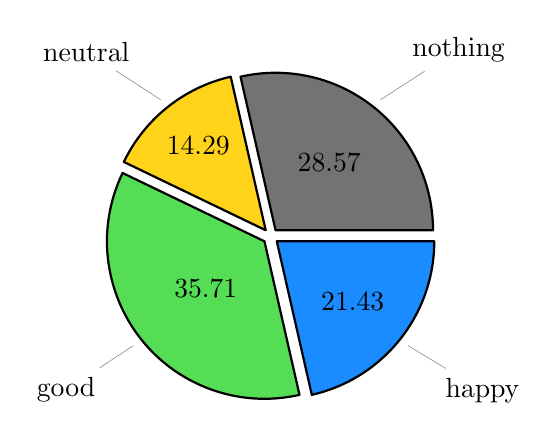
\begin{tikzpicture}
            \pie[text=legend, color={moodNothing, moodNeutral, moodGood, moodHappy}, radius=2, sum=auto, text=pin, explode={0.1, 0.1, 0.1, 0.1}]{
                28.57/nothing, 
                14.29/neutral, 
                35.71/good, 
                21.43/happy
            }
        \end{tikzpicture}
        \label{fig:`User 1'-welcome-mood}
    }
    \hfill
    \subfloat[User 2]{%
        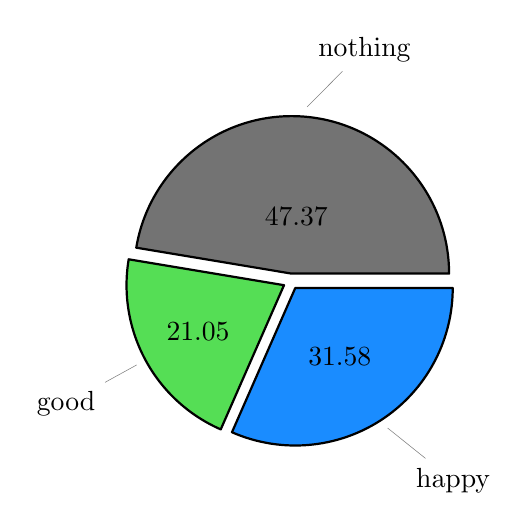
\begin{tikzpicture}
            \pie[text=legend, color={moodNothing, moodGood, moodHappy}, radius=2, sum=auto, text=pin, explode={0.1, 0.1, 0.1}]{
                47.37/nothing, 
                21.05/good, 
                31.58/happy
            }
        \end{tikzpicture}
        \label{fig:`User 2'-welcome-mood}
    }
\end{figure}
\FloatBarrier

\FloatBarrier
\begin{figure}[h!]\ContinuedFloat
    \centering
    \subfloat[User 3]{%
        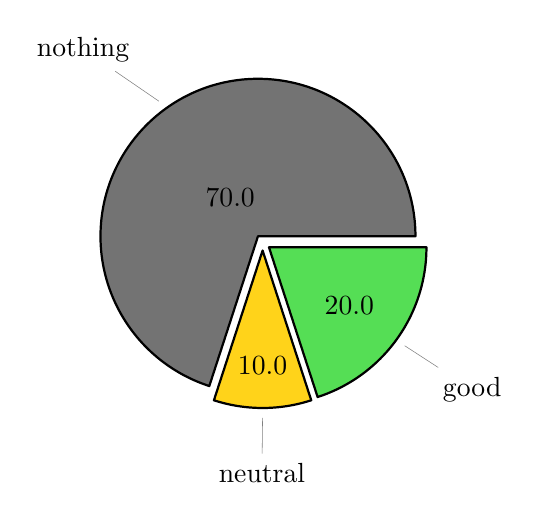
\begin{tikzpicture}
            \pie[text=legend, color={moodNothing, moodNeutral, moodGood}, radius=2, sum=auto, text=pin, explode={0.1, 0.1, 0.1}]{
                70.0/nothing, 
                10.0/neutral, 
                20.0/good
            }
        \end{tikzpicture}
        \label{fig:ioannis-welcome-mood}
    }
    \hfill
    \subfloat[User 4]{%
        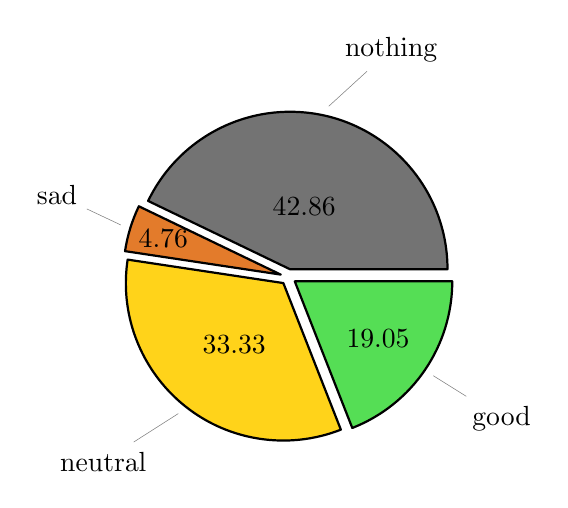
\begin{tikzpicture}
            \pie[text=legend, color={moodNothing, moodSad, moodNeutral, moodGood}, radius=2, sum=auto, text=pin, explode={0.1, 0.1, 0.1, 0.1}]{
                42.86/nothing, 
                4.76/sad, 
                33.33/neutral, 
                19.05/good
            }
        \end{tikzpicture}
        \label{fig:`User 4'-welcome-mood}
    }
\end{figure}
\FloatBarrier

\FloatBarrier
\begin{figure}[h!]\ContinuedFloat
    \centering
    \subfloat[User 5]{%
        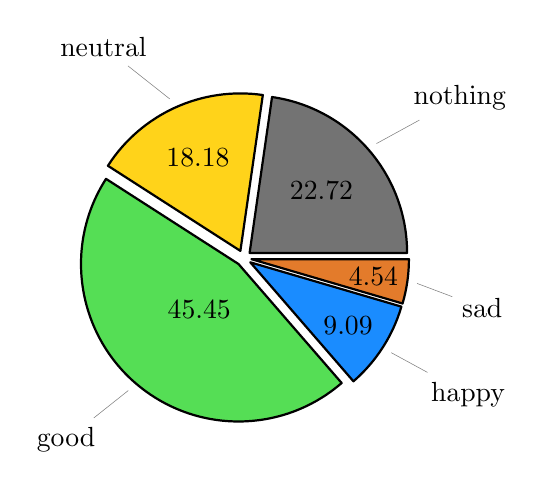
\begin{tikzpicture}
            \pie[text=legend, color={moodNothing, moodNeutral, moodGood, moodHappy, moodSad}, radius=2, sum=auto, text=pin, explode={0.1, 0.1, 0.1, 0.1, 0.1}]{
                22.72/nothing, 
                18.18/neutral, 
                45.45/good, 
                9.09/happy,
                4.54/sad
            }
        \end{tikzpicture}
        \label{fig:`User 5'-welcome-mood}
    }
    \hfill
    \subfloat[User 6]{%
        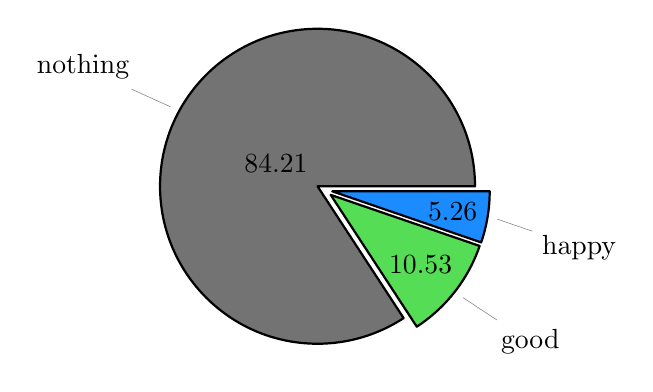
\begin{tikzpicture}
            \pie[text=legend, color={moodNothing, moodGood, moodHappy}, radius=2, sum=auto, text=pin, explode={0.1, 0.1}]{
                84.21/nothing, 
                10.53/good, 
                5.26/happy
            }
        \end{tikzpicture}
        \label{fig:`User 6'-welcome-mood}
    }
\end{figure}
\FloatBarrier

\FloatBarrier
\begin{figure}[h!]\ContinuedFloat
    \centering
    \subfloat[User 7]{%
        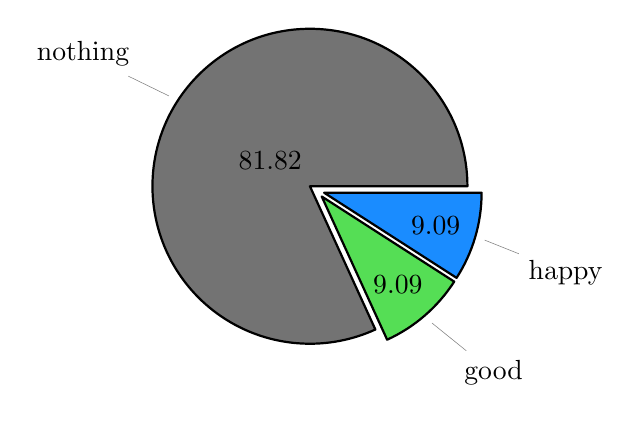
\begin{tikzpicture}
            \pie[text=legend, color={moodNothing, moodGood, moodHappy}, radius=2, sum=auto, text=pin, explode={0.1, 0.1, 0.1}]{
                81.82/nothing, 
                9.09/good, 
                9.09/happy
            }
        \end{tikzpicture}
        \label{fig:yiannis-welcome-mood}
    }
    \caption{Mood Distribution for Each User}
\end{figure}
\FloatBarrier

\vspace{5mm}

\noindent \textbf{Questionnaire Scores} \\
The figure below illustrates the scores obtained by each participant across different survey instances during the testing phase. Each colored bar represents the score of a specific survey, identified by its corresponding survey number in the legend. The height of the bars indicates the score achieved, with a maximum value of 26 for each survey. The x-axis displays the dates of each survey, while the y-axis shows the score values.\vspace{5mm} \\
This visualization provides an overview of the survey completion and engagement of each participant. Gaps or missing bars indicate periods when the participant did not complete a survey. This could be due to a variety of reasons, such as forgetting to take the survey, lack of time, or disinterest. Also a one day gap is natural, because the user finishes the survey, and the next day anew survey is being created. Additionally, variations in scores across surveys reflect the changes in participants' responses, potentially influenced by factors like daily mood fluctuations or external stressors, such as exams.

\vspace{5mm}

\FloatBarrier
\begin{figure}[ht]
    \centering
    \includegraphics[width=\linewidth]{figures/Figure-Scores.png}\label{fig:questionnaire-results}
    \caption{Questionnaire Results of the test users}
\end{figure}
\FloatBarrier

\vspace{5mm}

\subsection{Conclusion}

The results obtained during the testing phase show a diverse range of interactions and emotional responses from the participants, heavily influenced by their exam responsibilities. Participants with a more demanding exam schedule, such as \textbf{User 1} and \textbf{User 2}, exhibited higher frequencies of ``nothing'' and ``neutral'' welcome moods, indicating potential stress or lack of engagement during high-pressure periods. This trend is further supported by their questionnaire scores, which show considerable variability across different surveys, likely reflecting the fluctuations in their mental state as they navigated through challenging exams.\vspace{5mm} \\
Conversely, participants like \textbf{User 3} and \textbf{User 4}, who did not have any exams during the testing period, demonstrated more stable welcome mood distributions and consistent engagement in the daily surveys. This stability is echoed in their questionnaire scores, which did not exhibit the same level of fluctuation as those with heavier academic responsibilities.\vspace{5mm} \\
Interestingly, \textbf{User 5} and \textbf{User 6}, who faced a mix of intermediate and difficult courses, showed a more balanced distribution of welcome moods, with fewer ``nothing'' days compared to \textbf{User 1} and \textbf{User 2}. Their survey scores also reflect this balance, with some variations that indicate the challenges of their schedules without reaching the extremes seen in other participants.\vspace{5mm} \\
Additionally, it’s worth noting that several participants showed limited engagement with the application. This lack of engagement is evident in the frequency of “nothing” welcome moods and the low completion rates of the daily surveys. These findings suggest that participants may have been too occupied to fully engage with the app, highlighting the importance of addressing user motivation and commitment, especially during busy periods.\vspace{5mm} \\
Overall, the data points to a strong link between exam stress and mood, demonstrating how external factors can significantly impact emotional well-being and participation levels. By considering these factors, we can gain better insights into user behavior and adjust the application to offer more personalized support during high-stress times. This can ultimately make mood tracking more effective and reliable, catering better to users’ varying levels of engagement.
Overall, there is a clear link between exam stress and mood, as seen in many participants. This shows how external factors can significantly influence emotional well-being and survey responses. By considering these relationships, we can better understand the data and see how academic stress affects mood and participation. These insights help us improve the application to better support users during stressful times and make mood tracking more accurate and effective.

\section{Interviews}

To validate the conclusions drawn from the testing phase and gain deeper insight into the participants’ experiences with the application, individual interviews were conducted with each user. The purpose of these interviews was to explore their perspectives on the app's usability, overall experience, and its ability to accurately reflect their emotional states. By discussing about their moods during the user test phase, these interviews allowed us to confirm whether the application successfully depicted the participants’ actual moods and provided meaningful support for managing their well-being.

\subsection{Procedure}

During the testing phase, 7 out of the 9 participants actively used the application. However, only 6 participants were available for an interview, all except `User 3', and their feedback was gathered to gain a deeper understanding of their experiences with the app. A structured set of questions was prepared to cover a wide range of topics, including usability, user satisfaction, and areas of potential improvement. The questions aimed to gather feedback on various functionalities of the application and determine if it met the users' expectations. The questions asked during the interviews were as follows:

\begin{enumerate}
    \item \textbf{First impressions}: What were your initial thoughts before using the application? Was there any feature that stood out or surprised you, either positively or negatively?
    \item \textbf{Usage environment}: Where did you primarily use the application (e.g., at home, outdoors)? How would you describe your past three weeks—were they more stressful or relaxed?
    \item \textbf{Emotional impact}: How did you feel before and during the usage of the application? Did you feel obliged to use it, or was it something you engaged with naturally?
    \item \textbf{Ease of use}: Did you encounter any difficulties while using the app? Were there aspects that felt particularly challenging or, on the contrary, very straightforward?
    \item \textbf{Previous experience}: Have you used any similar applications in the past? If so, how would you compare your experience?
    \item \textbf{Feature feedback}: What features do you think are missing, or which ones require modifications?
    
    \vspace{2mm} If the participant did not address specific features, additional follow-up questions were asked:

    \begin{itemize}
        \item Was the content of the questionnaire appropriate and relevant?
        \item How did you feel about the questionnaire process and the frequency with which questions were repeated?
        \item Did you find the notifications helpful, or do you feel something was lacking?
    \end{itemize}
    
    \item \textbf{Frequency of use}: How often do you think you would use this application in your daily life?
    \item \textbf{Application summary}: How would you describe the application in one sentence or just a few words?
    \item \textbf{Additional comments}: Is there anything else you would like to add that we haven’t discussed?
\end{enumerate}

\noindent These questions provided a comprehensive view of the participants’ experiences and gathered valuable feedback to refine the application further.

\subsection{User Perspectives}

Based on the feedback collected from the user interviews, we can pinpoint various aspects of the application that users either appreciated or found areas for improvement.

\begin{enumerate}
    \item \textbf{First Impressions}
\end{enumerate}

\noindent Most participants were impressed by the design and interface of the application. Several users, like `User 1' and `User 2', highlighted the animation and visuals as a key feature that initially caught their attention. `User 4' mentioned that the immediate start of the welcome mood selection felt a bit abrupt but overall liked the simple and engaging interface. `User 6' described the design as ``really good'' and appreciated the quick loading time.

\begin{enumerate}[resume]
    \item \textbf{Usage Environment}
\end{enumerate}

\noindent Participants mainly used the application at home, with only a few trying it in other environments, such as cafés or while taking a walk. This pattern is primarily due to the exam period that many of them were going through, which limited their movement outside. For example, `User 2' used it at home 90\% of the time, while `User 5' occasionally used it outdoors.

\begin{enumerate}[resume]
    \item \textbf{Emotional Impact}
\end{enumerate}

\noindent The general aggrement between the users was that the application did not feel like an obligation or chore. However, `User 4' and `User 5' noted that as the days passed, the repetitive nature of the questions became a bit boring, making it feel less engaging over time. Participants like `User 7' found the app useful but felt that better use of data could enhance its impact on their mood management.

\begin{enumerate}[resume]
    \item \textbf{Ease of Use}
\end{enumerate}

\noindent Users found the application easy to navigate with clear guidance and large buttons. `User 1' described it as ``really simple, easy to use, and operational'', while `User 4' and `User 6' highlighted minor confusion at certain points, such as accidentally retaking surveys or understanding the purpose of some buttons. These initial usability issues resolved themselves with continued use.

\begin{enumerate}[resume]
    \item \textbf{Previous Experience}
\end{enumerate}

\noindent Most participants had not used similar applications before, making this their first exposure to a mood-tracking app. For example, `User 2' noted that he enjoyed the experience as it made him reflect on his day, something he wouldn’t usually do. `User 4' mentioned he wanted to use a similar app before, but the subscription-based nature discouraged him.

\begin{enumerate}[resume]
    \item \textbf{Feature Feedback}
\end{enumerate}

\noindent While most users appreciated the features, some specific recommendations were made for improvement:

\begin{itemize}
    \item \textbf{Questionnaire Content:} Several users felt that some of the questions were too extreme or repetitive. For instance, `User 5' and `User 7' suggested more general questions related to daily life rather than intense psychological states. `User 4' recommended a mix of certified and custom questions to keep the content balanced and engaging.

    \item \textbf{Survey Process and Frequency:} Some participants, such as `User 2', felt that the survey could be available earlier in the day, allowing more flexibility in responding. On the other hand, `User 1' suggested that the application should create the survey and notify the user during the evening, to better depict the user's overall daily mental health. `User 4' suggested adding a new question each day or refreshing the question set every few days to prevent monotony.

    \item \textbf{Notifications:} Notifications were generally appreciated for keeping users engaged. However, `User 1' and `User 4' suggested making them more personalized or playful, such as including emojis or varying text content.

    \item \textbf{Message Feature (Quotes/Advice):} The message feature received positive feedback for its motivational aspect, though users like `User 5' mentioned that at times the text color clashed with the background, making it hard to read.

    \item \textbf{Statistics:} There was some confusion around the bar chart, especially regarding the scores displayed. Participants were unsure about the meaning of low scores until it was explained to them. This highlighted a need for clearer communication of the results and scores.
\end{itemize}

\noindent The users also were asked about new features that they would like to see, so they proposed some ideas such as:

\begin{itemize}
    \item \textbf{Diary Feature:} `User 4' and `User 6' both suggested introducing a diary feature where users could write down their thoughts or capture daily insights, further enhancing the app's role as a personal mood tracker and journal.

    \item \textbf{Photo-Based Mood Capture:} `User 6' also proposed adding a feature similar to ``BeReal'' where users could capture and upload a photo every day to visually document their emotions, adding an additional dimension to mood tracking.

    \item \textbf{Gamification Elements:} Some participants suggested incorporating more gamification elements to make the experience more engaging. For example, `User 1' mentioned introducing streaks or achievements based on consistent usage, while `User 6' suggested including daily or weekly challenges that encourage user participation.

    \item \textbf{Adaptive Questionnaire Content:} Another suggestion was to implement adaptive questionnaires that adjust based on the user’s responses or history, gradually becoming more tailored to their personal experiences and mental state. This would ensure that the content remains relevant and engaging over time.
\end{itemize}

\begin{enumerate}[resume]
    \item \textbf{Frequency of Use}
\end{enumerate}

\noindent Participants expressed varied interest in using the application regularly. Those without exams or stressful schedules, such as `User 7' and `User 4', felt they could use the application daily. However, participants like `User 5' mentioned they might reduce their usage during exam periods due to time constraints.

\begin{enumerate}[resume]
    \item \textbf{Application Summary}
\end{enumerate}

\noindent Each user summarized the application in their own unique way, highlighting different aspects of their experience. `User 1' described it simply as ``My diary!'', emphasizing its role in tracking his day-to-day emotions. `User 6' offered a more detailed description, calling it: ``Delightful, innovative, and pioneering, which is well designed and constructed''. `User 4' viewed the app as ``Playful and engaging'', noting its potential for daily use if some improvements were made. `User 2' described it as ``Emotion'', reflecting how the app made him more aware of his mental state. `User 5' referred to it as ``Simple, accessible, and straightforward'', praising its user-friendly interface. `User 7' appreciated its potential value for mental health, describing it as ``Useful and promising''. Each participant's summary captures a different perspective, showcasing the diverse ways the application impacted their experience.

\begin{enumerate}[resume]
    \item \textbf{Additional Comments}
\end{enumerate}

\noindent No more comments, from the users, about the application, so the users were given the chance to ask any questions they had about the app, leading to insightful discussions about its features and potential future enhancements. Several participants expressed curiosity about different aspects of the app, such as its deployment process, the scoring system, and the possibility of adding new functionalities. This engagement provided a deeper understanding of how users perceived the app and what additional features they felt would improve their overall experience. For instance, `User 1' was interested in learning whether the application could evolve with new features based on user feedback. `User 5', on the other hand, was curious about the technical deployment process and the tools used, such as Docker and Google Cloud. `User 2' and `User 6' wanted clarification on how the questionnaire scores were calculated and how they correlated with their mental state. These discussions helped clarify certain functionalities and revealed areas for further development, making it clear that users were invested in understanding the application on a more detailed level.

\subsection{Conclusion}

The interviews provided valuable insight into how users perceived and interacted with the application. Across the nine different topics discussed, participants shared a mix of positive feedback and constructive suggestions for improvement. They appreciated the application's simple and intuitive design, its motivational message feature, and the ease of navigating the survey process. However, many pointed out areas that could be improved, like offering a wider range of questions, changing the timing and format of notifications, and allowing more flexibility with the survey schedule. Additionally, users highlighted the need for clearer communication of survey scores and results to enhance understanding of their mood trends over time.\vspace{5mm} \\
The interviews also confirmed that the application was generally successful in depicting participants’ actual moods during the testing phase. Although it did not capture their emotional states with complete accuracy, the app’s assessments were considered to be reflective of users' real moods  most of the times. This finding highlights the application’s potential as a reliable mood-tracking tool, while also emphasizing the importance of including more personalized elements to further enhance its accuracy.\vspace{5mm} \\
Suggestions for additional features, such as incorporating a diary or photo-based mood tracking option, were common among several users and indicate a desire for more personal and expressive ways to document their emotional states. The feedback on the questionnaire content, particularly the call for more balanced and less extreme questions, suggests an opportunity to make the app feel more relatable and less formal.\vspace{5mm} \\
Overall, the interviews strengthen the value of the application while shedding light on key areas for improvement. The insights gathered are important in guiding the next steps for development, ensuring that the application continues to meet user needs and provide meaningful support for mental health and well-being.

\section{UEQ Questionnaire}

To get a more complete evaluation of the application, I included the UEQ questionnaire. While the interviews provided good qualitative feedback, I needed a quantitative measure (with numbers) to confirm that users had a positive experience. The UEQ helped validate these results by capturing key aspects of the user experience in a structured way.\vspace{5mm} \\
The \textbf{\href{https://www.ueq-online.org/}{User Experience Questionnaire (UEQ)}}\footnote{\url{https://www.ueq-online.org/}} is a widely used tool for evaluating the user experience of interactive products. It offers valuable insights into how users perceive an application’s usability and user interface, by measuring six distinct dimensions: Attractiveness, Perspicuity, Efficiency, Dependability, Stimulation, and Novelty. These dimensions provide insights into both the pragmatic qualities (such as how easy it is to use the application) and hedonic qualities (such as how engaging or motivating the app is).

\subsection{Procedure}
For the evaluation of the application, six out of the nine user testers who participated in the previous testing phase and in the interviews phase were selected. These participants were chosen based on their level of engagement and consistent use of the application throughout the testing period. The remaining three participants were excluded from this evaluation due to their minimal usage and interaction with the application.\vspace{5mm} \\
The procedure for conducting the UEQ was straightforward and designed to minimize complexity for the participants. A Google Form was created, containing all the questions from the UEQ. This format was chosen to ensure that the questionnaire could be completed quickly and easily, without imposing additional time constraints on the users. The Google Form link was then shared with each participant through direct messages on various platforms such as Instagram, Messenger, and WhatsApp. This approach facilitated efficient communication and allowed participants to complete the questionnaire at their convenience.

\subsection{Results}
Based on the results provided by the UEQ questionnaire, we can derive some key insights about the user experience of the application. The UEQ measures different aspects of user experience using a variety of scales such as Attractiveness, Perspicuity (ease of understanding and learning), Efficiency, Dependability, Stimulation, and Novelty. So the concluding text for each of the scales is shown below:

\begin{enumerate}
    \item \textbf{Overall Attractiveness}: The responses indicate that the application is generally considered attractive by the users. This suggests a positive perception of the application's visual design, layout, and overall appeal.
    \item \textbf{Perspicuity (Ease of Use)}: Participants rated the application as understandable and easy to learn, indicating that users did not struggle with comprehending the features or navigation. This suggests that the application is intuitive and well-organized.
    \item \textbf{Efficiency}: Users considered the application efficient, which reflects that they felt it was effective in achieving its purpose without unnecessary complexity or time wastage.
    \item \textbf{Dependability}: The scores show that the users found the application dependable. This dimension is associated with users' perceptions of control, security, and predictability of the application.
    \item \textbf{Stimulation (Excitement and Engagement)}: The results were mixed for this category, suggesting that while some users found the application stimulating and engaging, others found it somewhat repetitive. This could be linked to the feedback from interviews about the need for more variety in the questionnaires or features.
    \item \textbf{Novelty (Innovation and Creativity)}: The novelty scores suggest that the application was seen as somewhat conventional. Users appreciated its innovative elements but may have felt that additional creative features or more dynamic interactions could further enhance their experience.
\end{enumerate}

\subsection{Conclusion}
The UEQ results validate the findings from the interviews by confirming that the application is user-friendly, easy to understand, and visually appealing. However, there is room for improvement in the areas of stimulation and novelty. Introducing new features, varying the questions, or adding interactive elements could address these aspects, making the application more engaging and less repetitive.

\section{Discussion}

The evaluation using \textbf{User Testing}, \textbf{Individual Interviews}, and the \textbf{User Experience Questionnaire (UEQ)} provided a complete view of the application's performance, usability, and effectiveness in meeting its primary objective. Each method revealed key insights into how the application supports students in tracking and managing their mood.

\subsection{Overall Findings}

The \textbf{User Testing} phase showed that participants were generally able to interact with the app independently after a short learning period, highlighting its ease of use and accessibility. Despite minor issues, the overall experience was positive, confirming the app's usability.\vspace{5mm} \\
The \textbf{Interviews} validated that the application captured participants’ moods accurately most of the time. Users appreciated its simple design but suggested enhancements such as adding a diary feature or more diverse content to better reflect their emotional states. These suggestions indicate that while the app performs well, additional personalization would improve its effectiveness.\vspace{5mm} \\
The \textbf{UEQ} results comfirmed these observations, showing high scores in usability and attractiveness but lower scores in engagement and novelty. This suggests that while the app is user-friendly and functional, there is room for improvement in keeping users engaged over time.

\subsection{Achievement of Primary Objective}

The primary objective, which was mentioned in the first chapter, was to create a tool that helps students track their mood and manage their well-being. The evaluation confirms that the app achieved this goal by providing a platform for mood tracking and reflection. Although it didn’t capture moods with complete accuracy, the application was able to depict the users' emotional states in a high percentage of cases, making it a reliable tool for mood tracking.

\subsection{Areas for Improvement}

The evaluation highlighted areas for further development, including more adaptive questionnaires, a diary feature, and improved data visualization. Addressing these aspects could make the application more engaging and responsive to users’ needs.

\section{Conclusion}

The evaluation results confirm that the developed application successfully provides students with a practical tool for tracking their mood and well-being throughout their academic journey. Through the combined use of \textbf{User Testing}, \textbf{Interviews}, and the \textbf{UEQ}, the app demonstrated strong usability, an intuitive interface, and the ability to depict users' emotional states with reasonable accuracy. Although certain areas, such as engagement and personalization, require further refinement, the overall feedback suggests that the app has achieved its primary objective of supporting students' mental health. Moving forward, incorporating user suggestions and more adaptive features will be crucial to enhancing the app's impact and ensuring it remains a relevant and valuable tool for students.

\chapter{Conclusion}

This thesis presents a comprehensive study on enhancing student mental health in higher education through the development of a mood-tracking application. The research focused on identifying key factors influencing well-being and implementing a system that could monitor these variables through daily surveys and assessments. The application was designed with user-centered principles, including intuitive interfaces and seamless data management. The proposed solution is adaptable to various university environments, providing valuable insights into students' emotional states and contributing to a more supportive academic community.

\section{Synopsis of the thesis}

The thesis followed a structured approach to address the problem of student mental health by developing an application that provides mood tracking and support. Initially, a detailed literature review was conducted to identify the core issues and understand existing solutions in the field. This was followed by an in-depth analysis using frameworks like the PACT model, along with personas and user scenarios, which laid the groundwork for understanding user needs and defining the application’s initial direction.\vspace{5mm} \\
The design phase focused on defining the user experience, incorporating elements like colors, fonts, and interface layouts to create a user-friendly environment. Design inspirations were drawn from existing solutions, and mockups and prototypes were developed for each screen of the application. The aim was to ensure a complete and intuitive experience that aligns with user expectations.\vspace{5mm} \\
During the implementation phase, the database was designed using ERD and UML diagrams to structure the data efficiently, the Xata platform for implmenting the application's database, while the front-end and back-end were developed using appropriate frameworks and technologies, such as React Native and Express respectively. The deployment was handled through cloud services, ensuring scalability and stability of the system.\vspace{5mm} \\
Finally, the application was evaluated using both expert-based and user-based methods. A specialized questionnaire (UEQ) and structured interviews were conducted to gather feedback, which was then used to assess the effectiveness and usability of the application. The evaluation highlighted areas for improvement and validated the system’s potential to support student well-being effectively.

\section{Future Steps}

Based on the evaluation of the application, valuable feedback and suggestions for improvement have been collected. Future developments may include refining the application’s functionality and design, adding some new features which were proposed by the users during their interviews, optimizing deployment for platforms like the App Store and Play Store, and potentially offering the application as a resource for universities to support student mental health. Expanding the application's reach and usability will contribute to better engagement and effectiveness in addressing mental health challenges in higher education environments.

\printbibliography[heading=bibintoc, title={Bibliography}]
\end{document}